% Options for packages loaded elsewhere
\PassOptionsToPackage{unicode}{hyperref}
\PassOptionsToPackage{hyphens}{url}
\PassOptionsToPackage{dvipsnames,svgnames,x11names}{xcolor}
%
\documentclass[
  letterpaper,
  DIV=11,
  numbers=noendperiod,
  titlepage]{scrartcl}

\usepackage{amsmath,amssymb}
\usepackage{iftex}
\ifPDFTeX
  \usepackage[T1]{fontenc}
  \usepackage[utf8]{inputenc}
  \usepackage{textcomp} % provide euro and other symbols
\else % if luatex or xetex
  \usepackage{unicode-math}
  \defaultfontfeatures{Scale=MatchLowercase}
  \defaultfontfeatures[\rmfamily]{Ligatures=TeX,Scale=1}
\fi
\usepackage{lmodern}
\ifPDFTeX\else  
    % xetex/luatex font selection
\fi
% Use upquote if available, for straight quotes in verbatim environments
\IfFileExists{upquote.sty}{\usepackage{upquote}}{}
\IfFileExists{microtype.sty}{% use microtype if available
  \usepackage[]{microtype}
  \UseMicrotypeSet[protrusion]{basicmath} % disable protrusion for tt fonts
}{}
\makeatletter
\@ifundefined{KOMAClassName}{% if non-KOMA class
  \IfFileExists{parskip.sty}{%
    \usepackage{parskip}
  }{% else
    \setlength{\parindent}{0pt}
    \setlength{\parskip}{6pt plus 2pt minus 1pt}}
}{% if KOMA class
  \KOMAoptions{parskip=half}}
\makeatother
\usepackage{xcolor}
\usepackage[top=20mm,bottom=5mm]{geometry}
\setlength{\emergencystretch}{3em} % prevent overfull lines
\setcounter{secnumdepth}{-\maxdimen} % remove section numbering
% Make \paragraph and \subparagraph free-standing
\ifx\paragraph\undefined\else
  \let\oldparagraph\paragraph
  \renewcommand{\paragraph}[1]{\oldparagraph{#1}\mbox{}}
\fi
\ifx\subparagraph\undefined\else
  \let\oldsubparagraph\subparagraph
  \renewcommand{\subparagraph}[1]{\oldsubparagraph{#1}\mbox{}}
\fi


\providecommand{\tightlist}{%
  \setlength{\itemsep}{0pt}\setlength{\parskip}{0pt}}\usepackage{longtable,booktabs,array}
\usepackage{calc} % for calculating minipage widths
% Correct order of tables after \paragraph or \subparagraph
\usepackage{etoolbox}
\makeatletter
\patchcmd\longtable{\par}{\if@noskipsec\mbox{}\fi\par}{}{}
\makeatother
% Allow footnotes in longtable head/foot
\IfFileExists{footnotehyper.sty}{\usepackage{footnotehyper}}{\usepackage{footnote}}
\makesavenoteenv{longtable}
\usepackage{graphicx}
\makeatletter
\def\maxwidth{\ifdim\Gin@nat@width>\linewidth\linewidth\else\Gin@nat@width\fi}
\def\maxheight{\ifdim\Gin@nat@height>\textheight\textheight\else\Gin@nat@height\fi}
\makeatother
% Scale images if necessary, so that they will not overflow the page
% margins by default, and it is still possible to overwrite the defaults
% using explicit options in \includegraphics[width, height, ...]{}
\setkeys{Gin}{width=\maxwidth,height=\maxheight,keepaspectratio}
% Set default figure placement to htbp
\makeatletter
\def\fps@figure{htbp}
\makeatother

\usepackage{booktabs}
\usepackage{longtable}
\usepackage{array}
\usepackage{multirow}
\usepackage{wrapfig}
\usepackage{float}
\usepackage{colortbl}
\usepackage{pdflscape}
\usepackage{tabu}
\usepackage{threeparttable}
\usepackage{threeparttablex}
\usepackage[normalem]{ulem}
\usepackage{makecell}
\usepackage{xcolor}
\usepackage{typearea}
\usepackage{caption}
\usepackage{subcaption}
\KOMAoption{captions}{tableheading}
\makeatletter
\makeatother
\makeatletter
\makeatother
\makeatletter
\@ifpackageloaded{caption}{}{\usepackage{caption}}
\AtBeginDocument{%
\ifdefined\contentsname
  \renewcommand*\contentsname{Table of contents}
\else
  \newcommand\contentsname{Table of contents}
\fi
\ifdefined\listfigurename
  \renewcommand*\listfigurename{List of Figures}
\else
  \newcommand\listfigurename{List of Figures}
\fi
\ifdefined\listtablename
  \renewcommand*\listtablename{List of Tables}
\else
  \newcommand\listtablename{List of Tables}
\fi
\ifdefined\figurename
  \renewcommand*\figurename{Figure}
\else
  \newcommand\figurename{Figure}
\fi
\ifdefined\tablename
  \renewcommand*\tablename{Table}
\else
  \newcommand\tablename{Table}
\fi
}
\@ifpackageloaded{float}{}{\usepackage{float}}
\floatstyle{ruled}
\@ifundefined{c@chapter}{\newfloat{codelisting}{h}{lop}}{\newfloat{codelisting}{h}{lop}[chapter]}
\floatname{codelisting}{Listing}
\newcommand*\listoflistings{\listof{codelisting}{List of Listings}}
\makeatother
\makeatletter
\@ifpackageloaded{caption}{}{\usepackage{caption}}
\@ifpackageloaded{subcaption}{}{\usepackage{subcaption}}
\makeatother
\makeatletter
\@ifpackageloaded{tcolorbox}{}{\usepackage[skins,breakable]{tcolorbox}}
\makeatother
\makeatletter
\@ifundefined{shadecolor}{\definecolor{shadecolor}{rgb}{.97, .97, .97}}
\makeatother
\makeatletter
\makeatother
\makeatletter
\makeatother
\ifLuaTeX
  \usepackage{selnolig}  % disable illegal ligatures
\fi
\IfFileExists{bookmark.sty}{\usepackage{bookmark}}{\usepackage{hyperref}}
\IfFileExists{xurl.sty}{\usepackage{xurl}}{} % add URL line breaks if available
\urlstyle{same} % disable monospaced font for URLs
\hypersetup{
  pdftitle={Simulation Result For Three-Level Intercept Model With Low Prevalence},
  pdfauthor={Shafayet Khan Shafee},
  colorlinks=true,
  linkcolor={blue},
  filecolor={Maroon},
  citecolor={Blue},
  urlcolor={Blue},
  pdfcreator={LaTeX via pandoc}}

\title{Simulation Result For Three-Level Intercept Model With Low
Prevalence}
\usepackage{etoolbox}
\makeatletter
\providecommand{\subtitle}[1]
\author{Shafayet Khan Shafee}
\date{07 September 2023}

\begin{document}
\maketitle
\ifdefined\Shaded\renewenvironment{Shaded}{\begin{tcolorbox}[frame hidden, interior hidden, borderline west={3pt}{0pt}{shadecolor}, enhanced, breakable, boxrule=0pt, sharp corners]}{\end{tcolorbox}}\fi

\hypertarget{histograms-for-logwidehatmor}{%
\section{\texorpdfstring{Histograms for
\(log(\widehat{MOR})\)}{Histograms for log(\textbackslash widehat\{MOR\})}}\label{histograms-for-logwidehatmor}}

\begin{figure}
\centering
\begin{subfigure}{.49\textwidth}
    \centering
    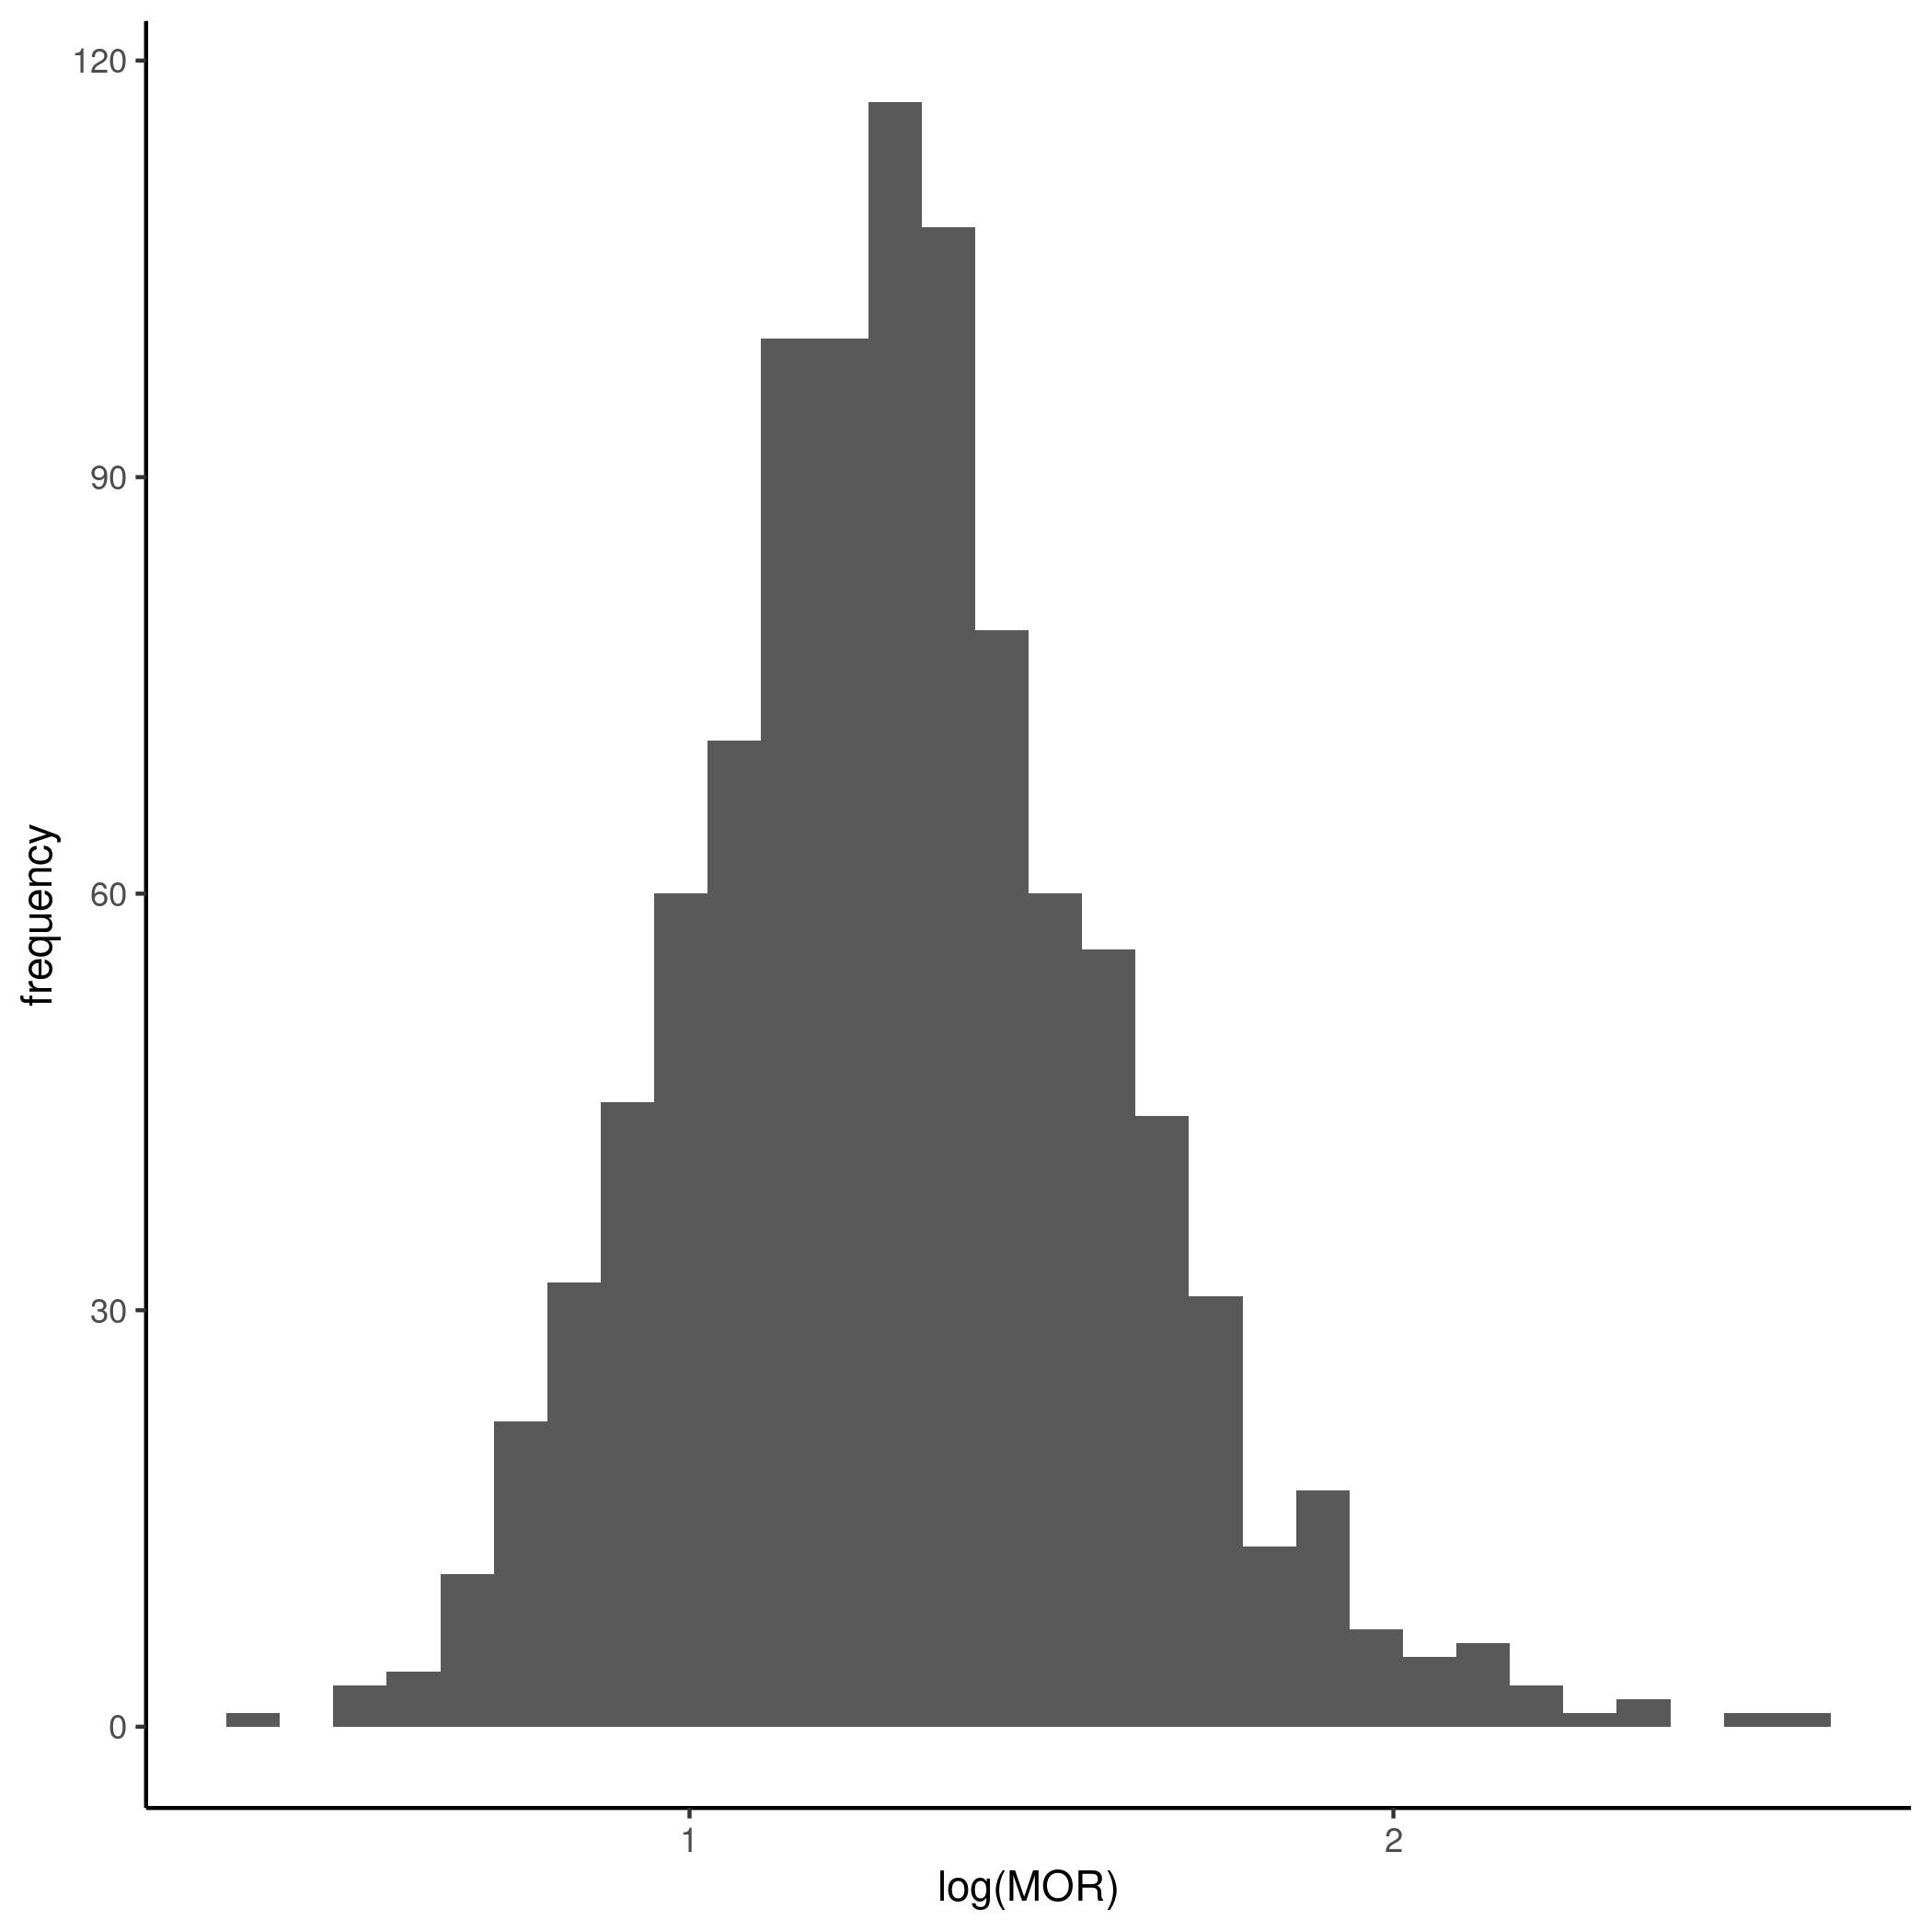
\includegraphics[width=.95\linewidth]{../../plots/three-lvl-ran-int/low-prev/hist_20_10_5_three_lvl_low_prev_mor1.png}  
    \caption{MOR\textsubscript{1}}
    \label{l20m10n51}
\end{subfigure}
\begin{subfigure}{.49\textwidth}
    \centering
    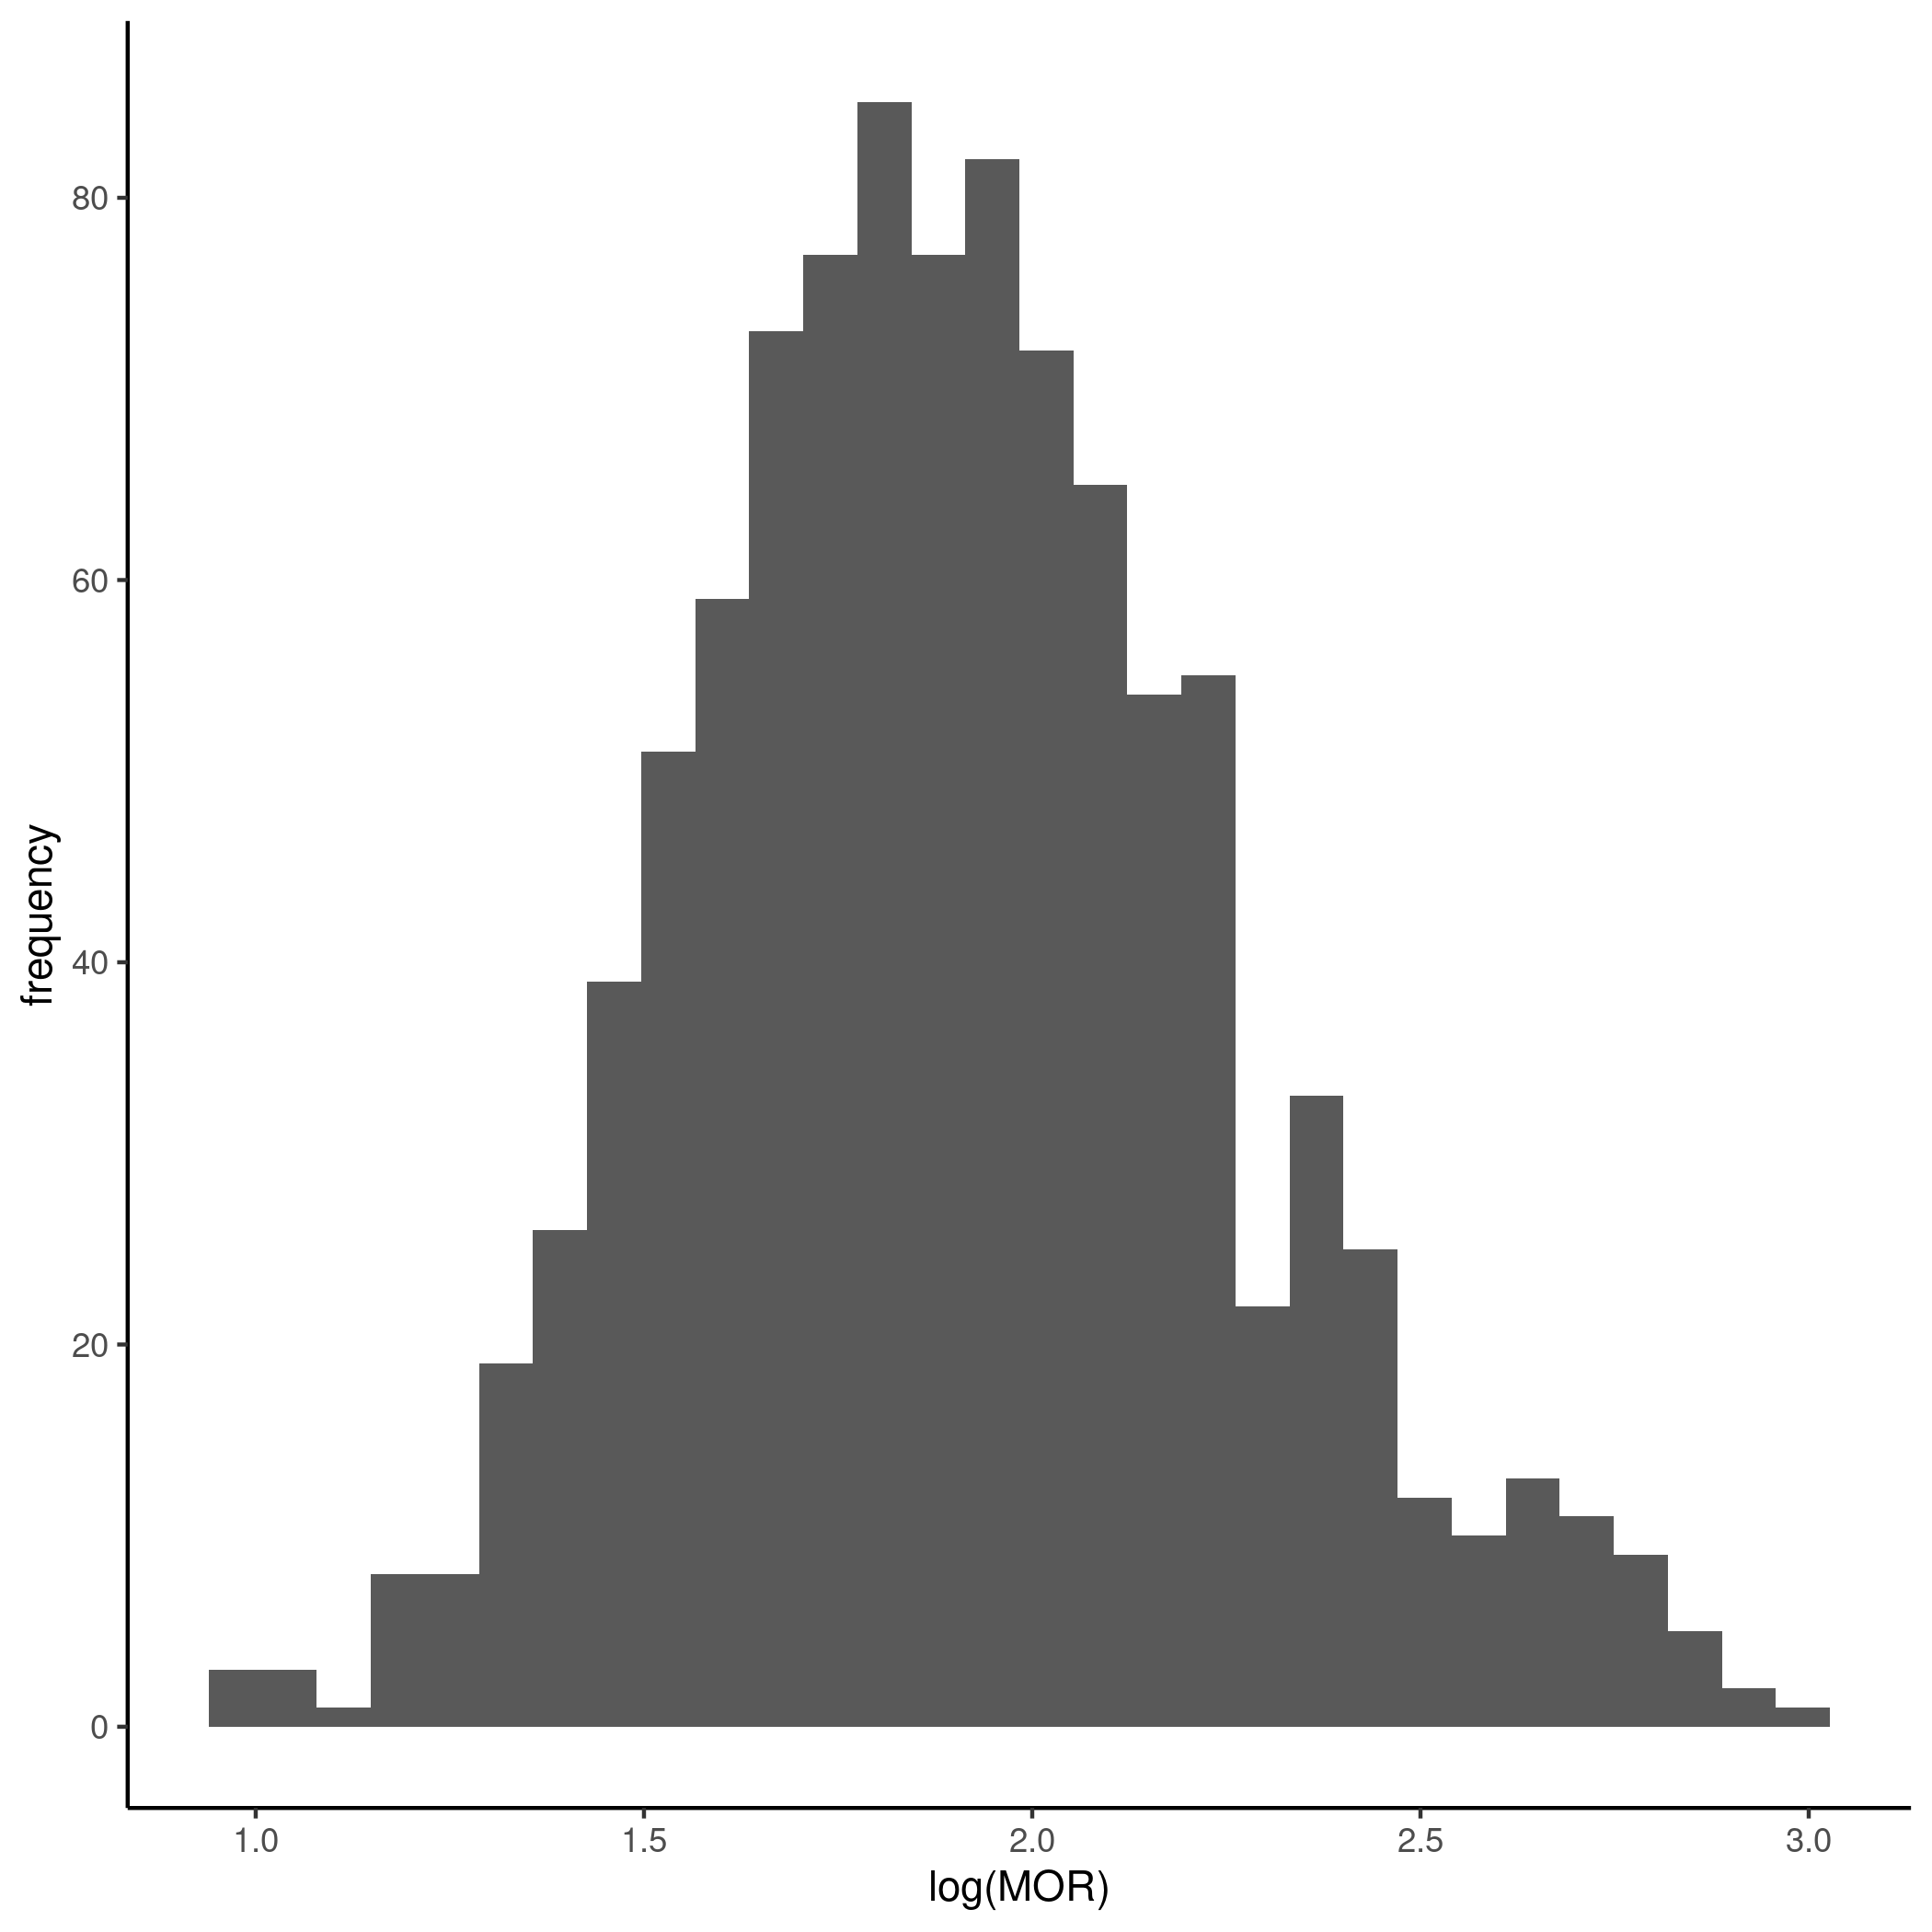
\includegraphics[width=.95\linewidth]{../../plots/three-lvl-ran-int/low-prev/hist_20_10_5_three_lvl_low_prev_mor2.png}  
    \caption{MOR\textsubscript{2}}
    \label{l20m10n52}
\end{subfigure}
\caption{Hospitals = 20, Doctors = 10, Patients = 5}
\label{mor1}
\end{figure}

\vspace{10mm}

\begin{figure}
\centering
\begin{subfigure}{.49\textwidth}
    \centering
    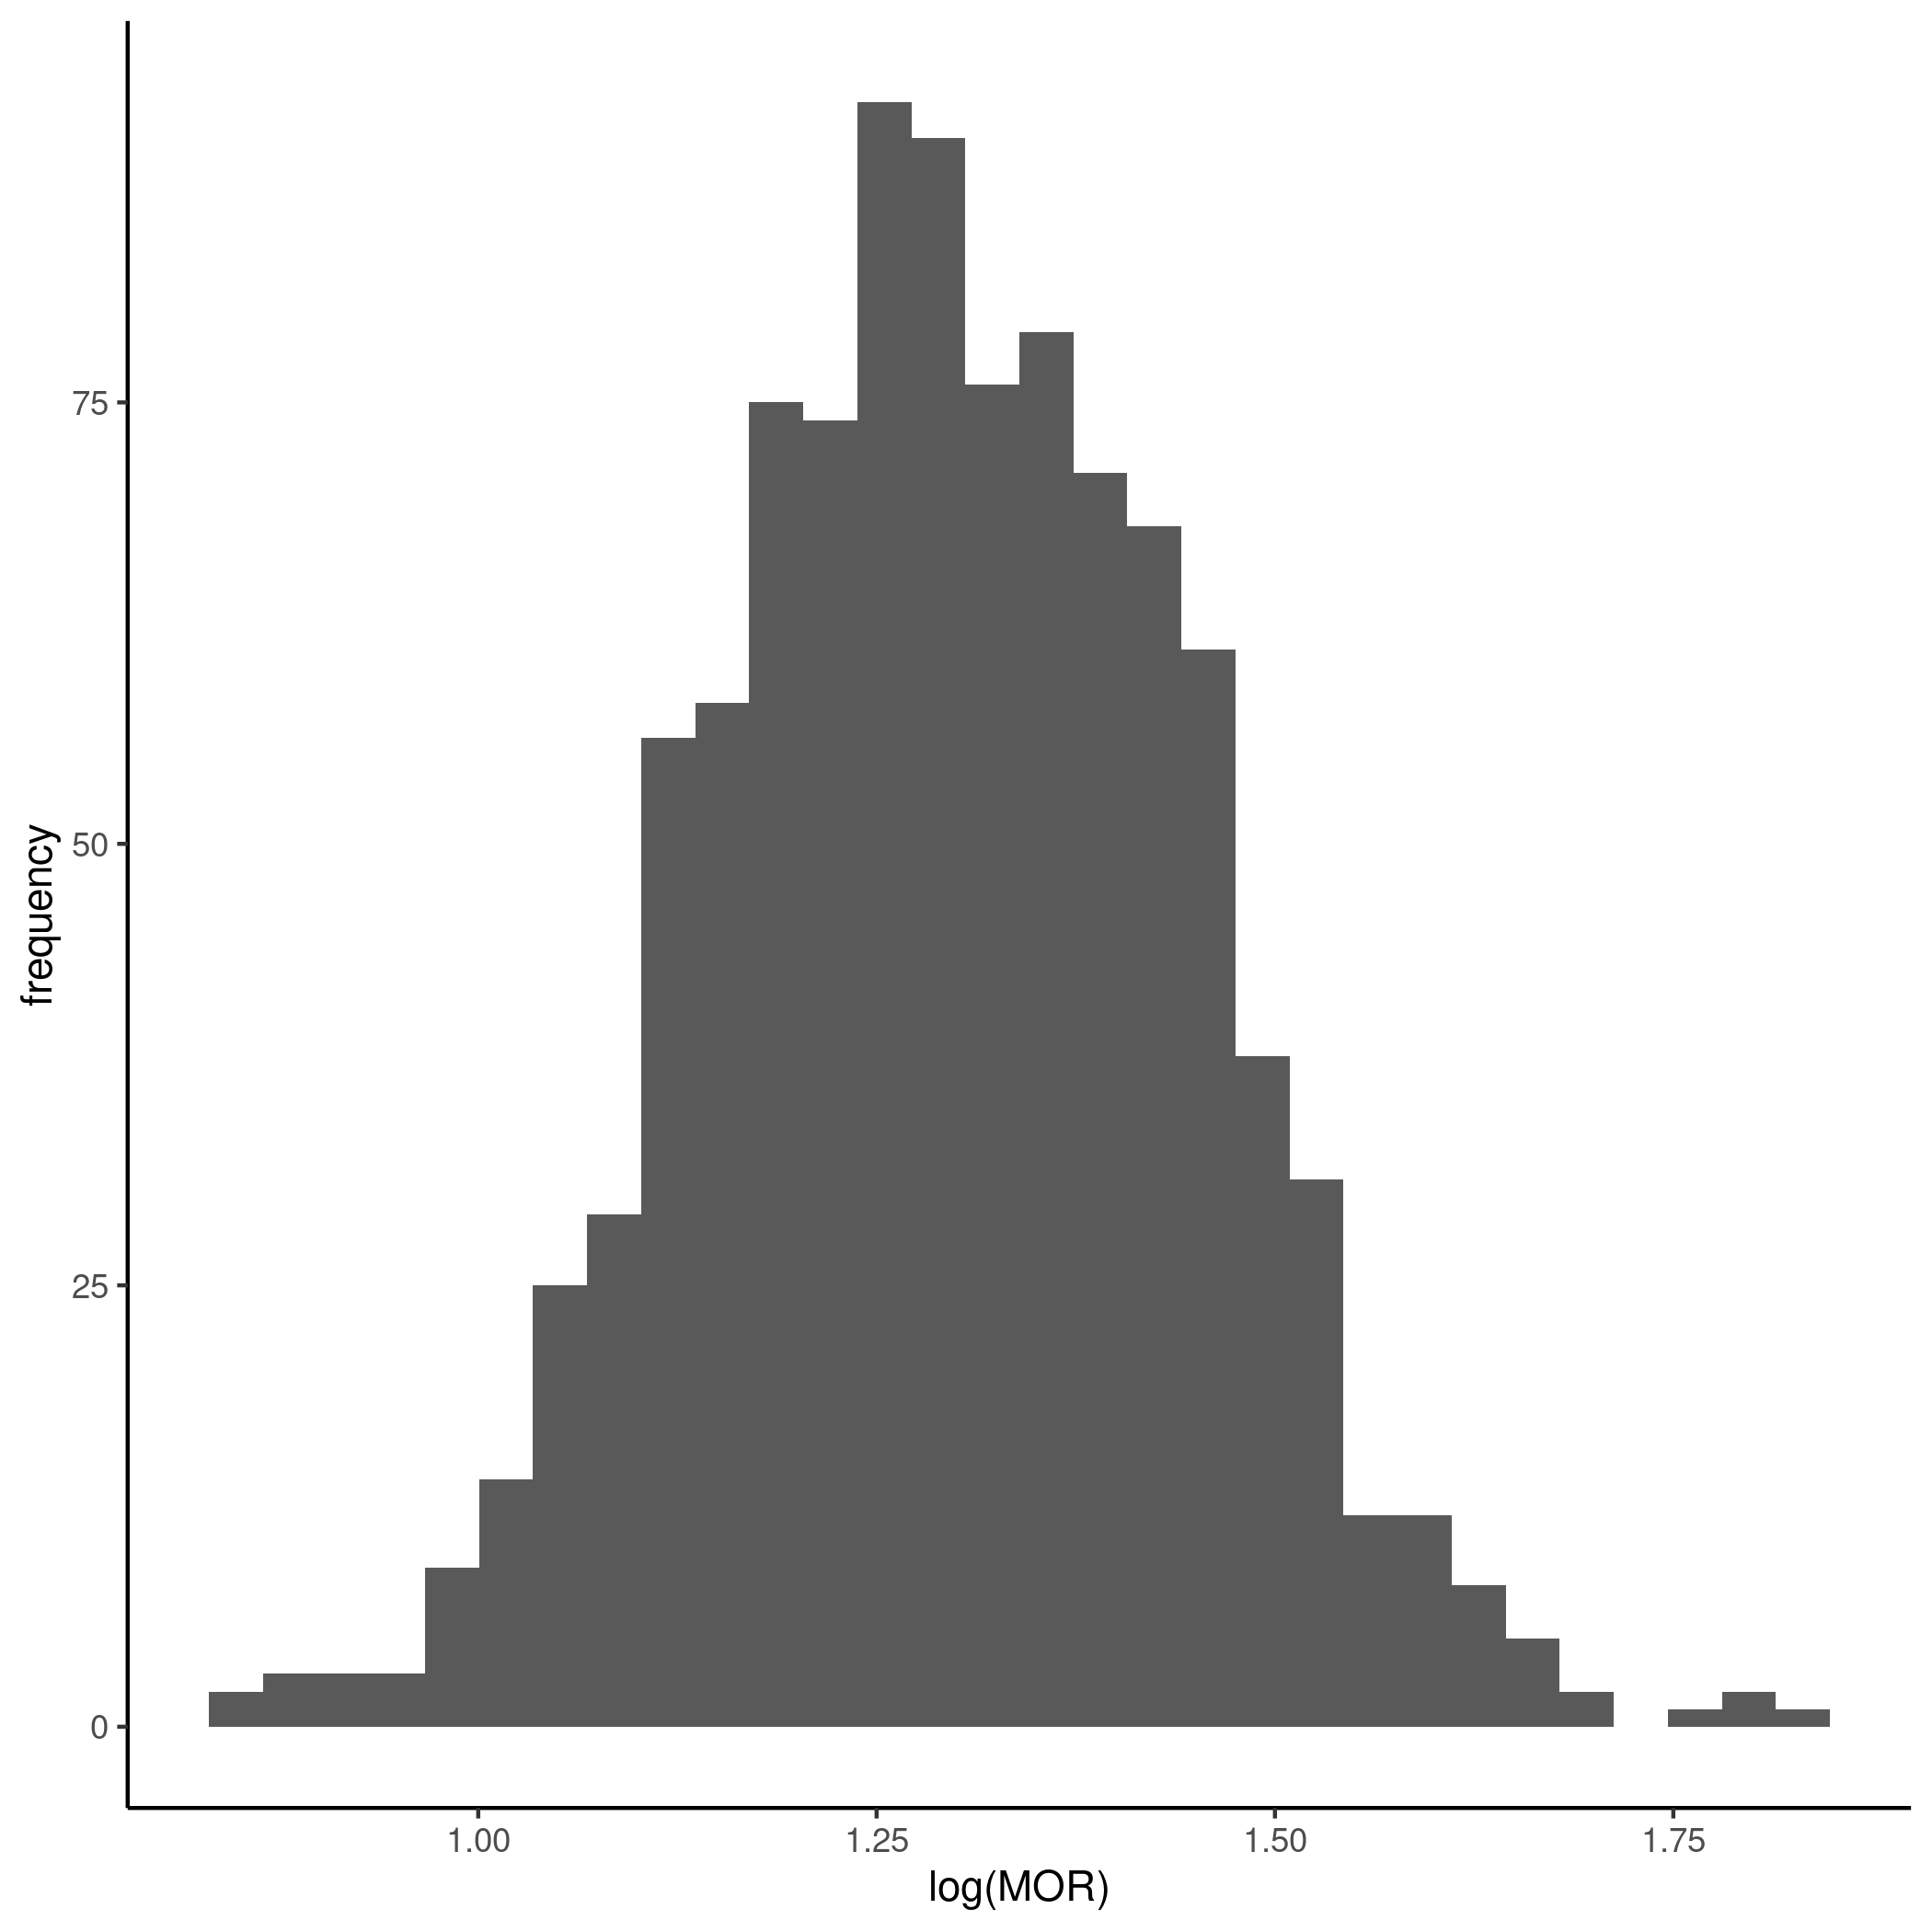
\includegraphics[width=.95\linewidth]{../../plots/three-lvl-ran-int/low-prev/hist_20_10_15_three_lvl_low_prev_mor1.png}  
    \caption{MOR\textsubscript{1}}
    \label{l20m10n151}
\end{subfigure}
\begin{subfigure}{.49\textwidth}
    \centering
    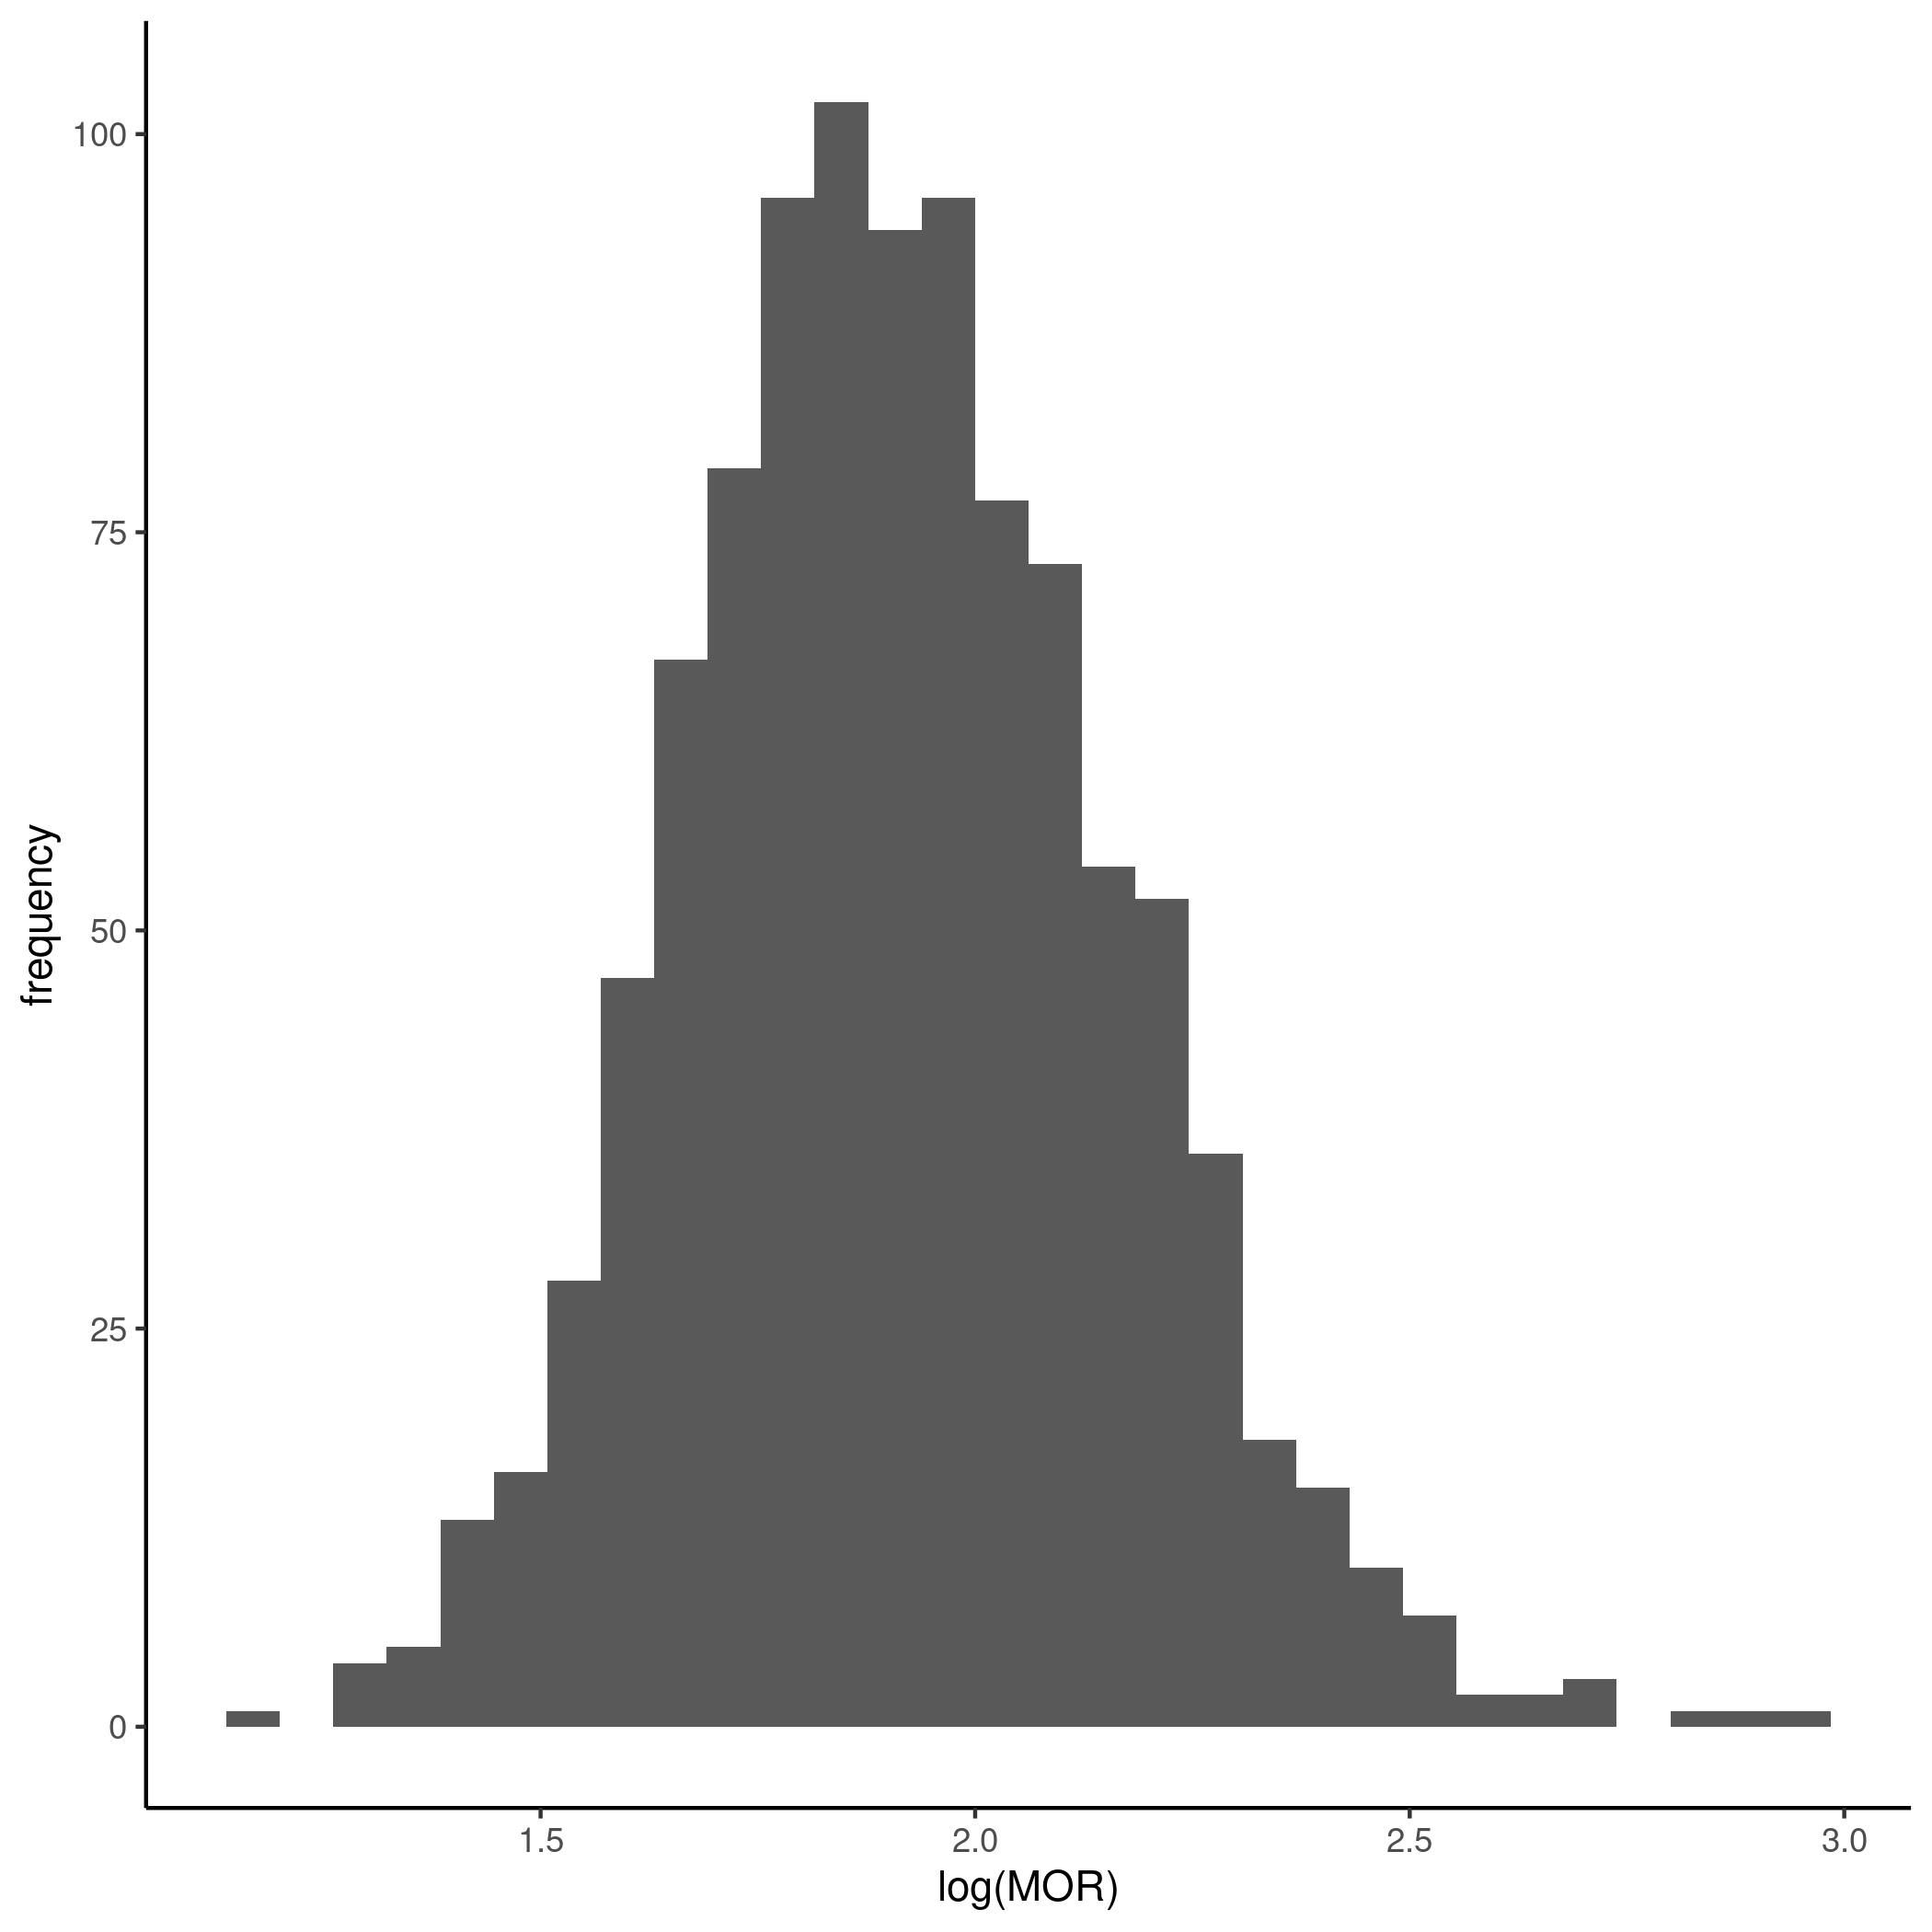
\includegraphics[width=.95\linewidth]{../../plots/three-lvl-ran-int/low-prev/hist_20_10_15_three_lvl_low_prev_mor2.png}  
    \caption{MOR\textsubscript{2}}
    \label{l20m10n152}
\end{subfigure}
\caption{Hospitals = 20, Doctors = 10, Patients = 15}
\label{mor1}
\end{figure}

\vspace{10mm}

\begin{figure}
\centering
\begin{subfigure}{.49\textwidth}
    \centering
    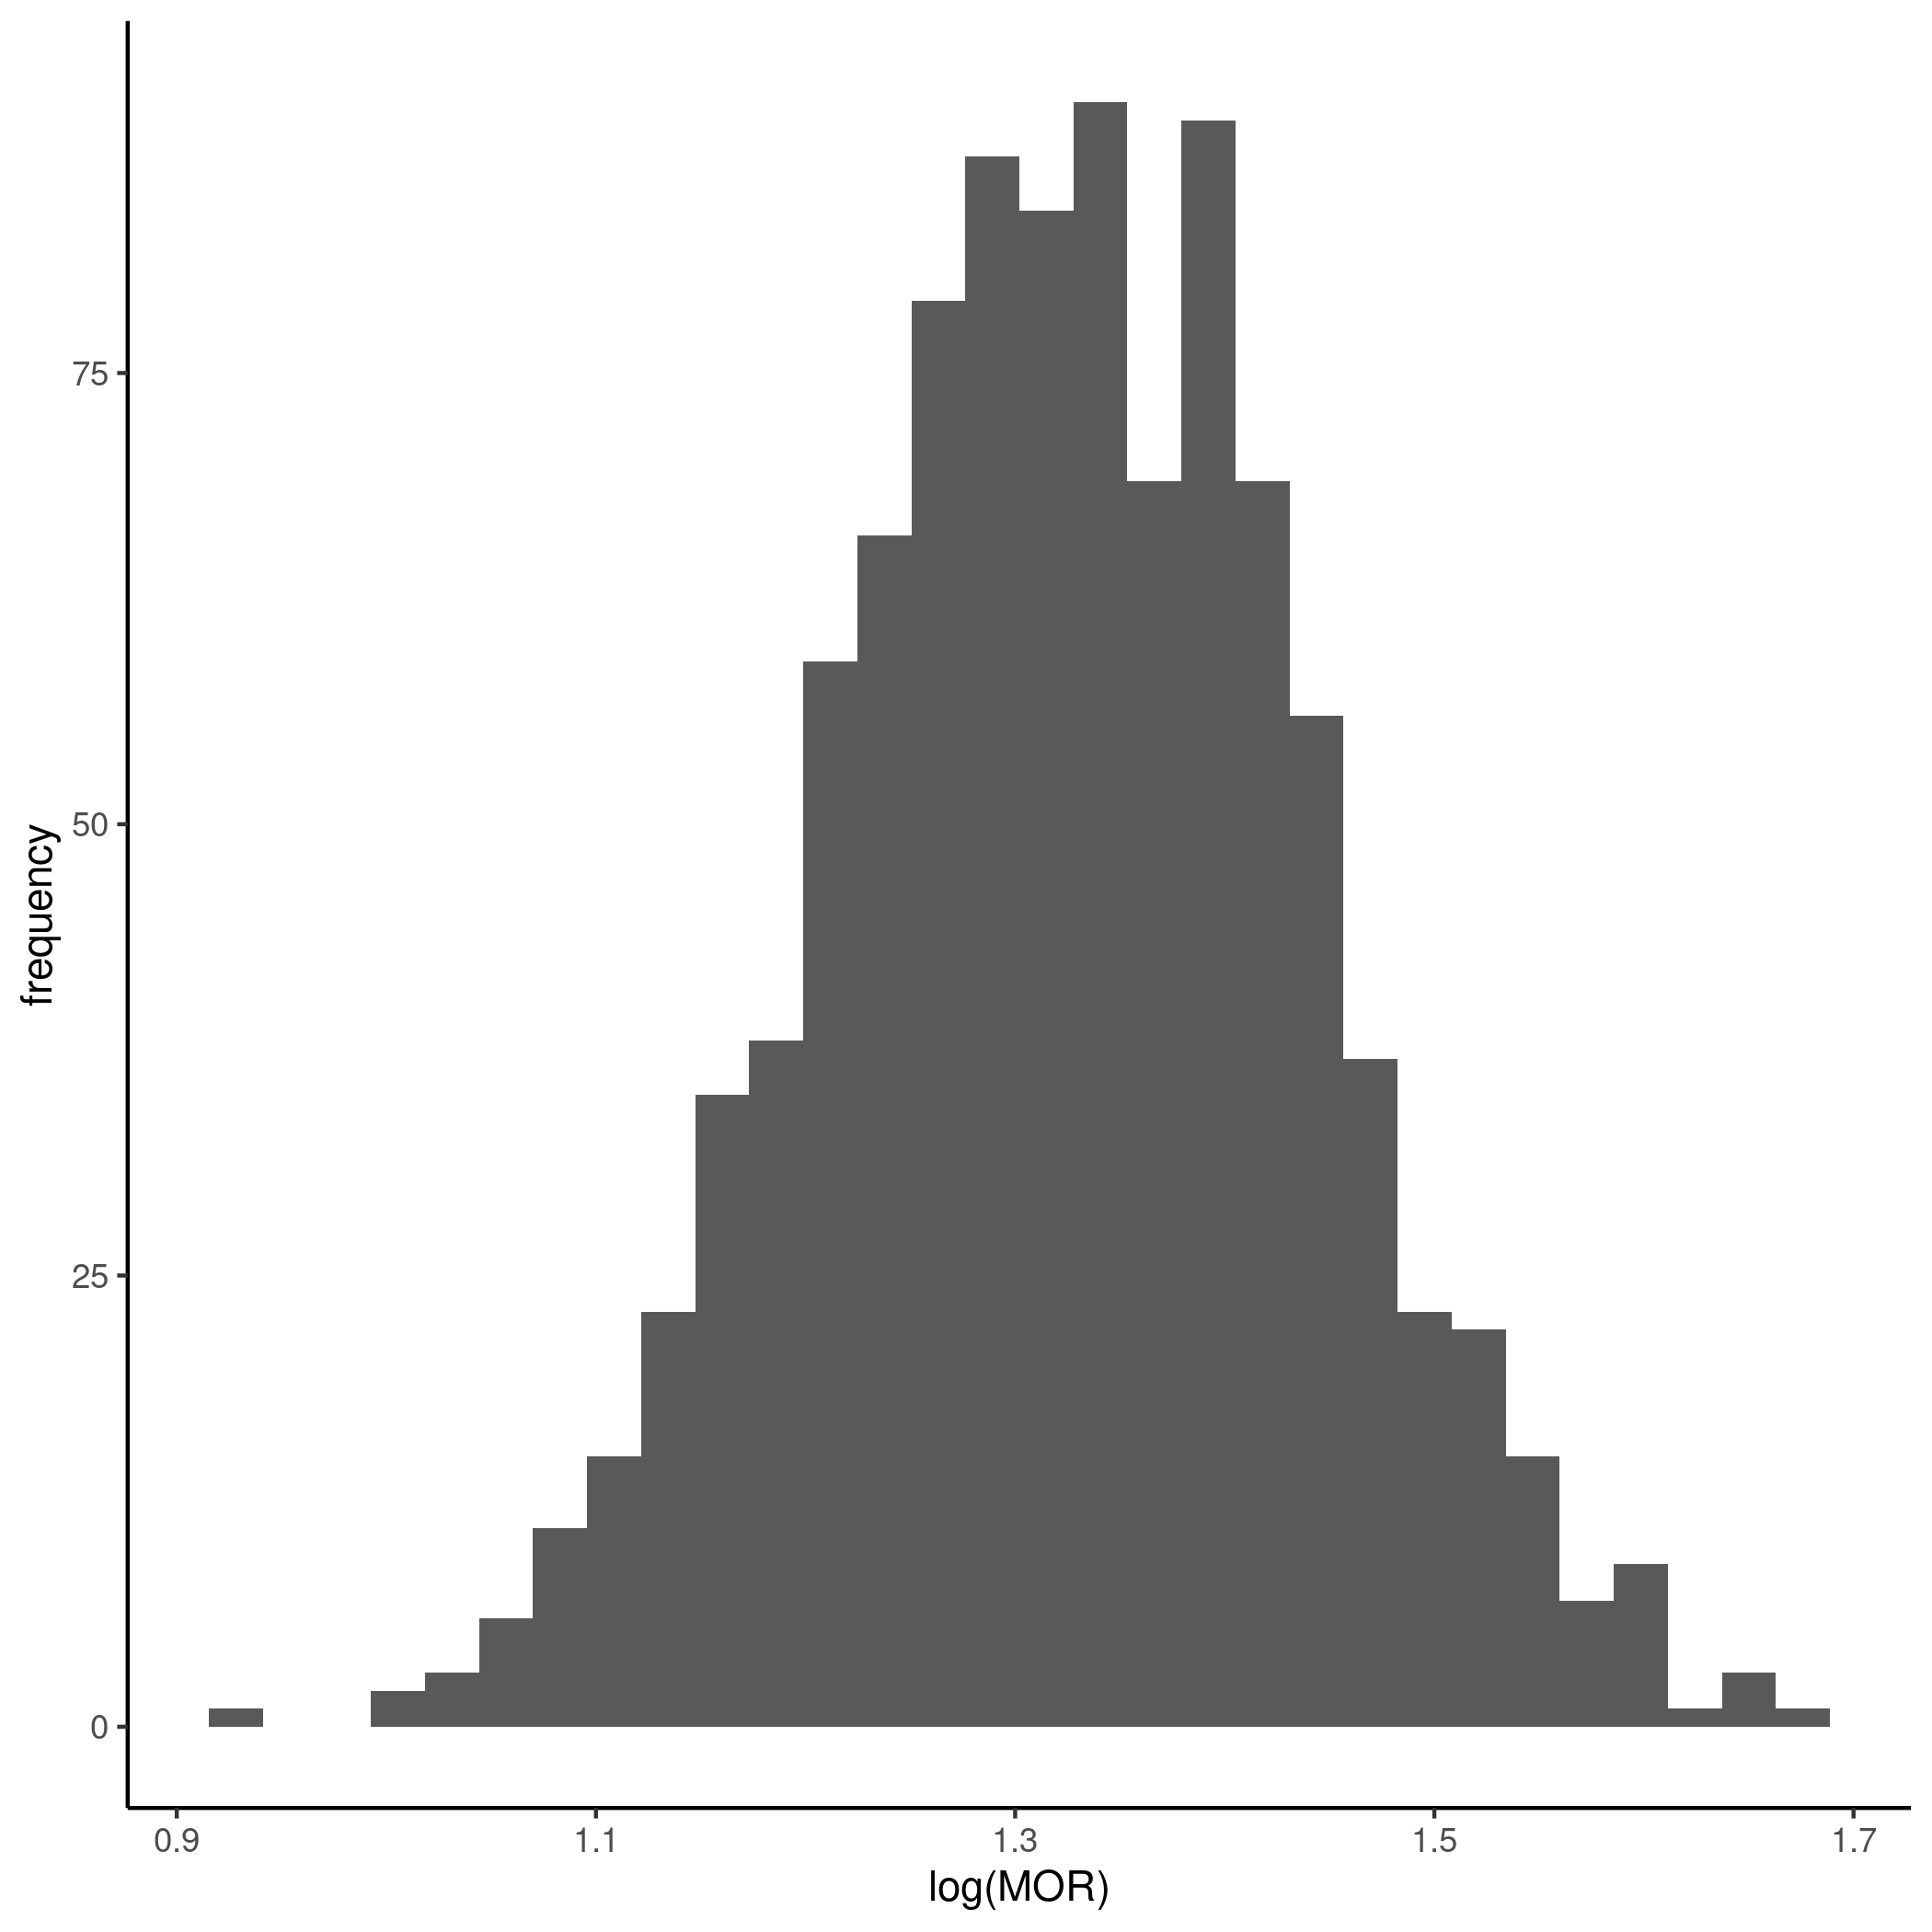
\includegraphics[width=.95\linewidth]{../../plots/three-lvl-ran-int/low-prev/hist_20_10_30_three_lvl_low_prev_mor1.png}  
    \caption{MOR\textsubscript{1}}
    \label{l20m10n151}
\end{subfigure}
\begin{subfigure}{.49\textwidth}
    \centering
    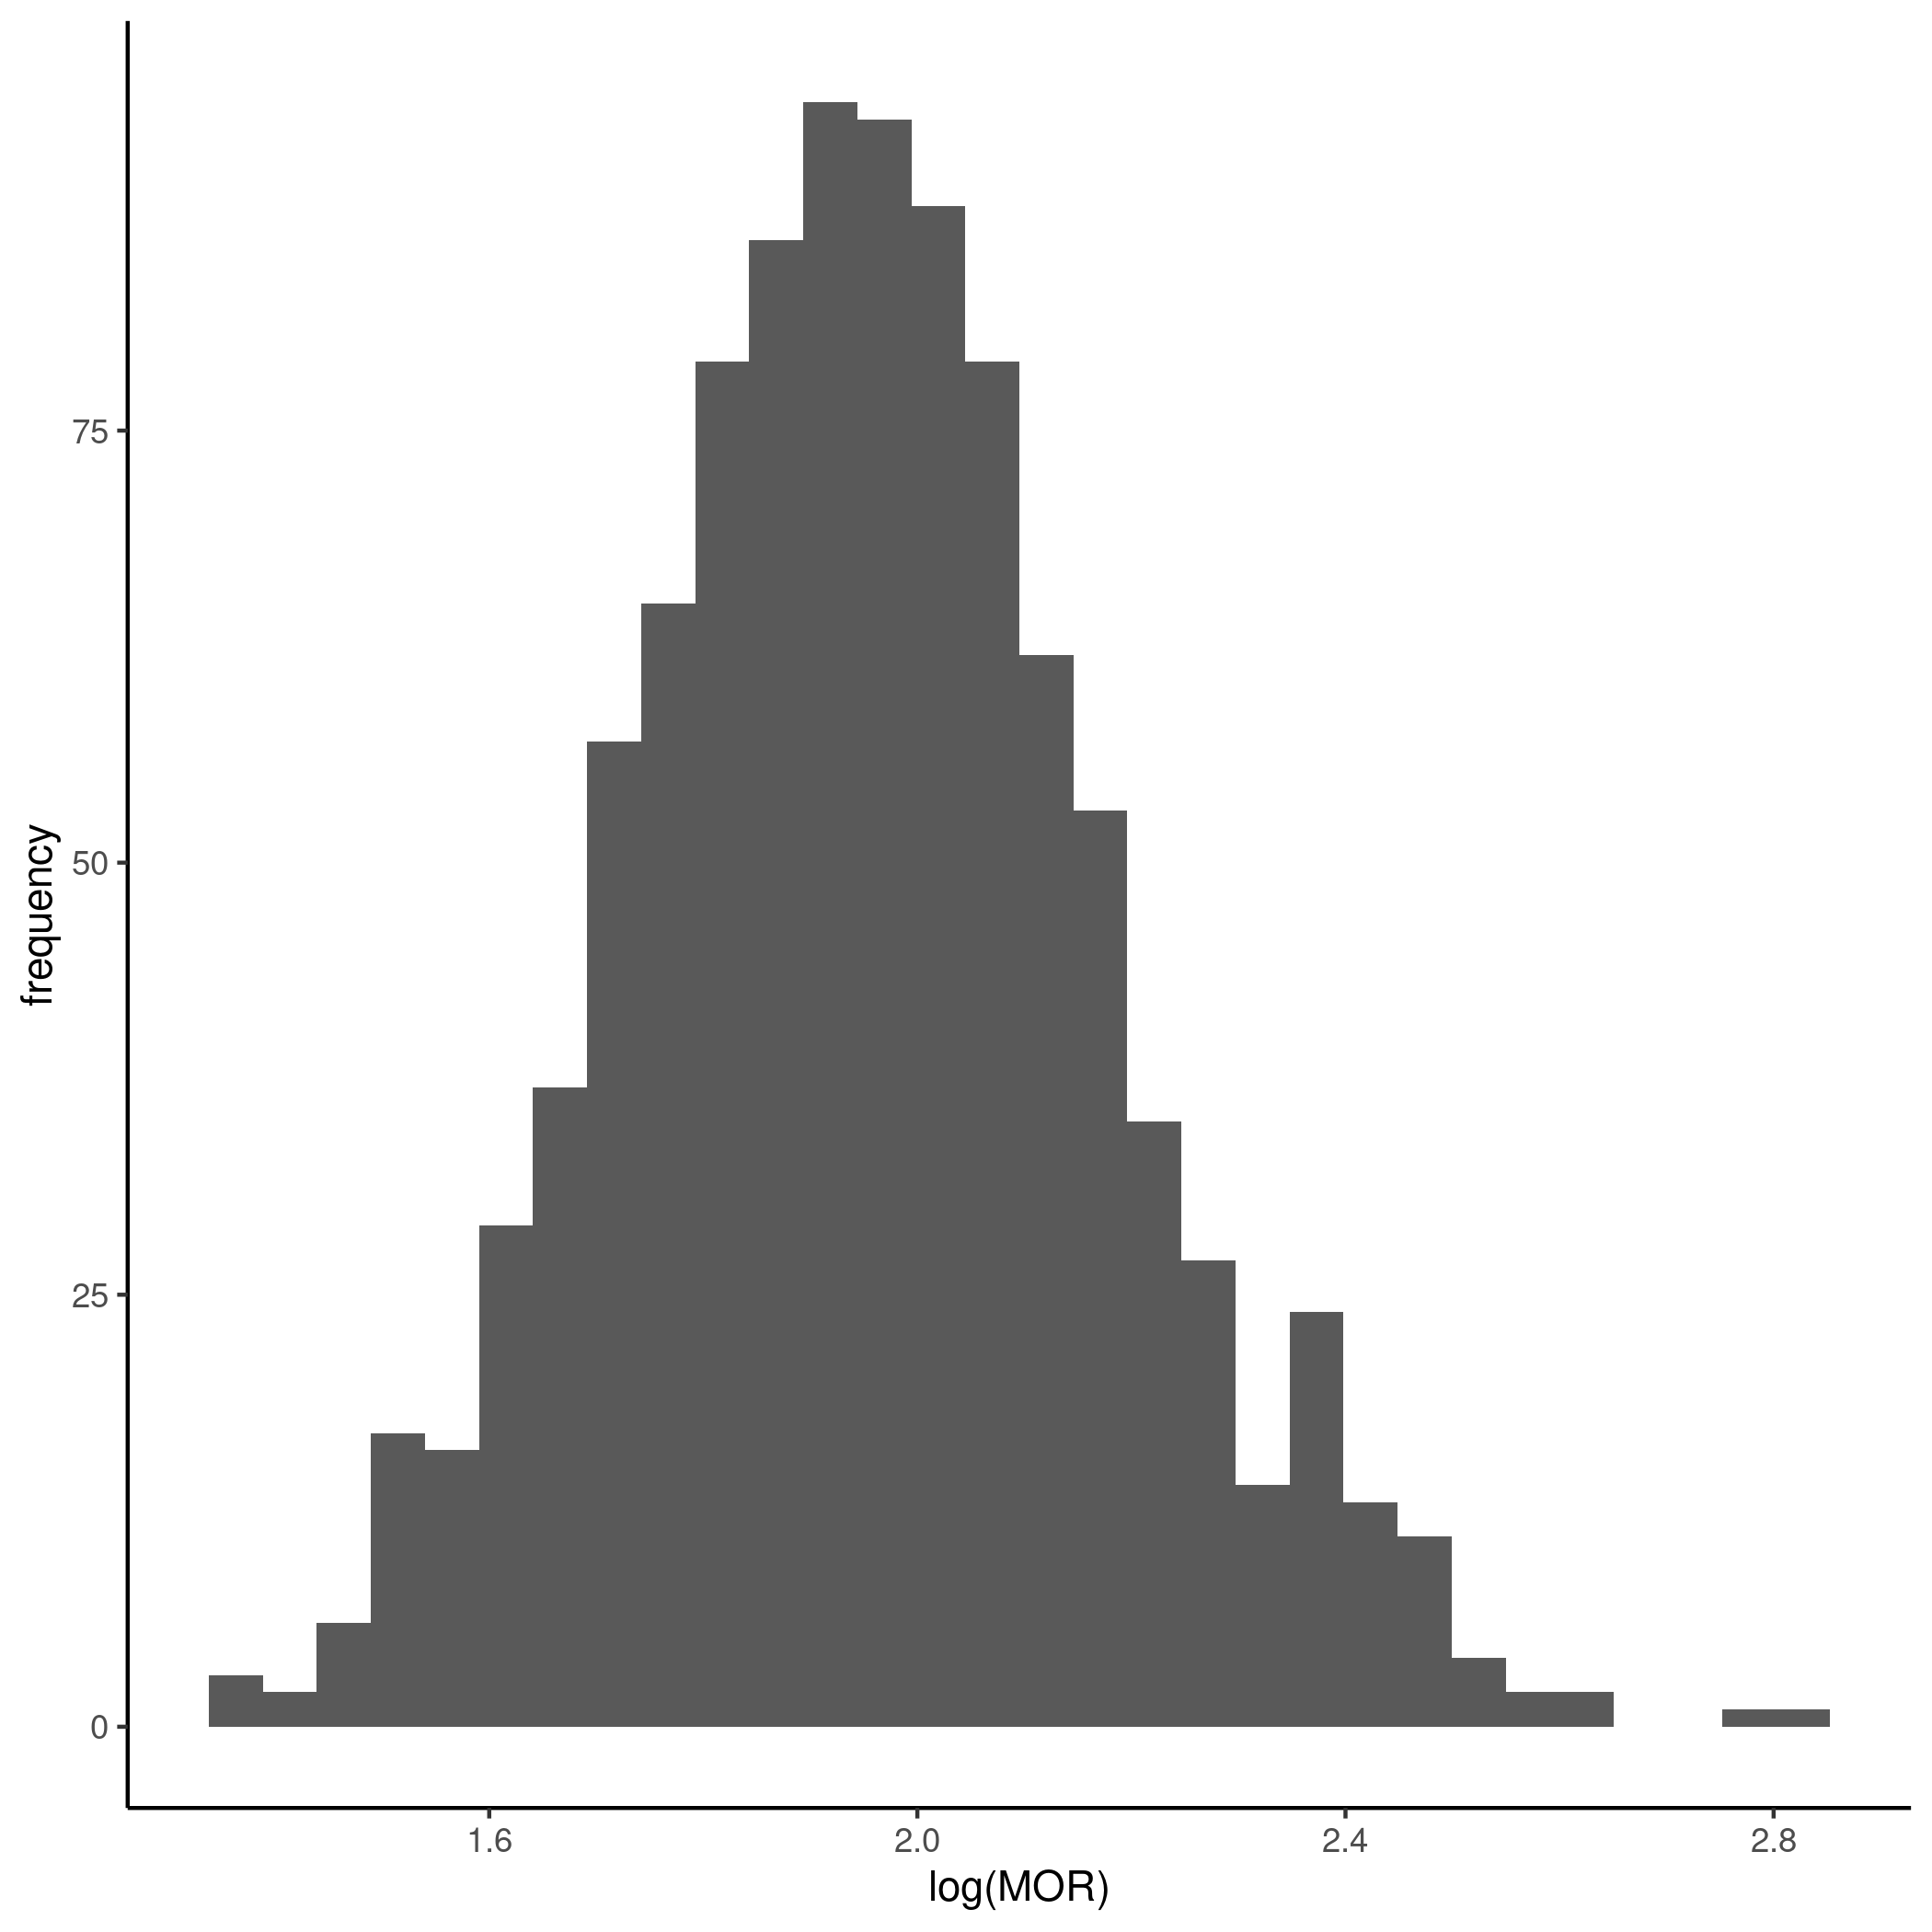
\includegraphics[width=.95\linewidth]{../../plots/three-lvl-ran-int/low-prev/hist_20_10_30_three_lvl_low_prev_mor2.png}  
    \caption{MOR\textsubscript{2}}
    \label{l20m10n152}
\end{subfigure}
\caption{Hospitals = 20, Doctors = 10, Patients = 30}
\label{mor1}
\end{figure}

\vspace{10mm}

\begin{figure}
\centering
\begin{subfigure}{.49\textwidth}
    \centering
    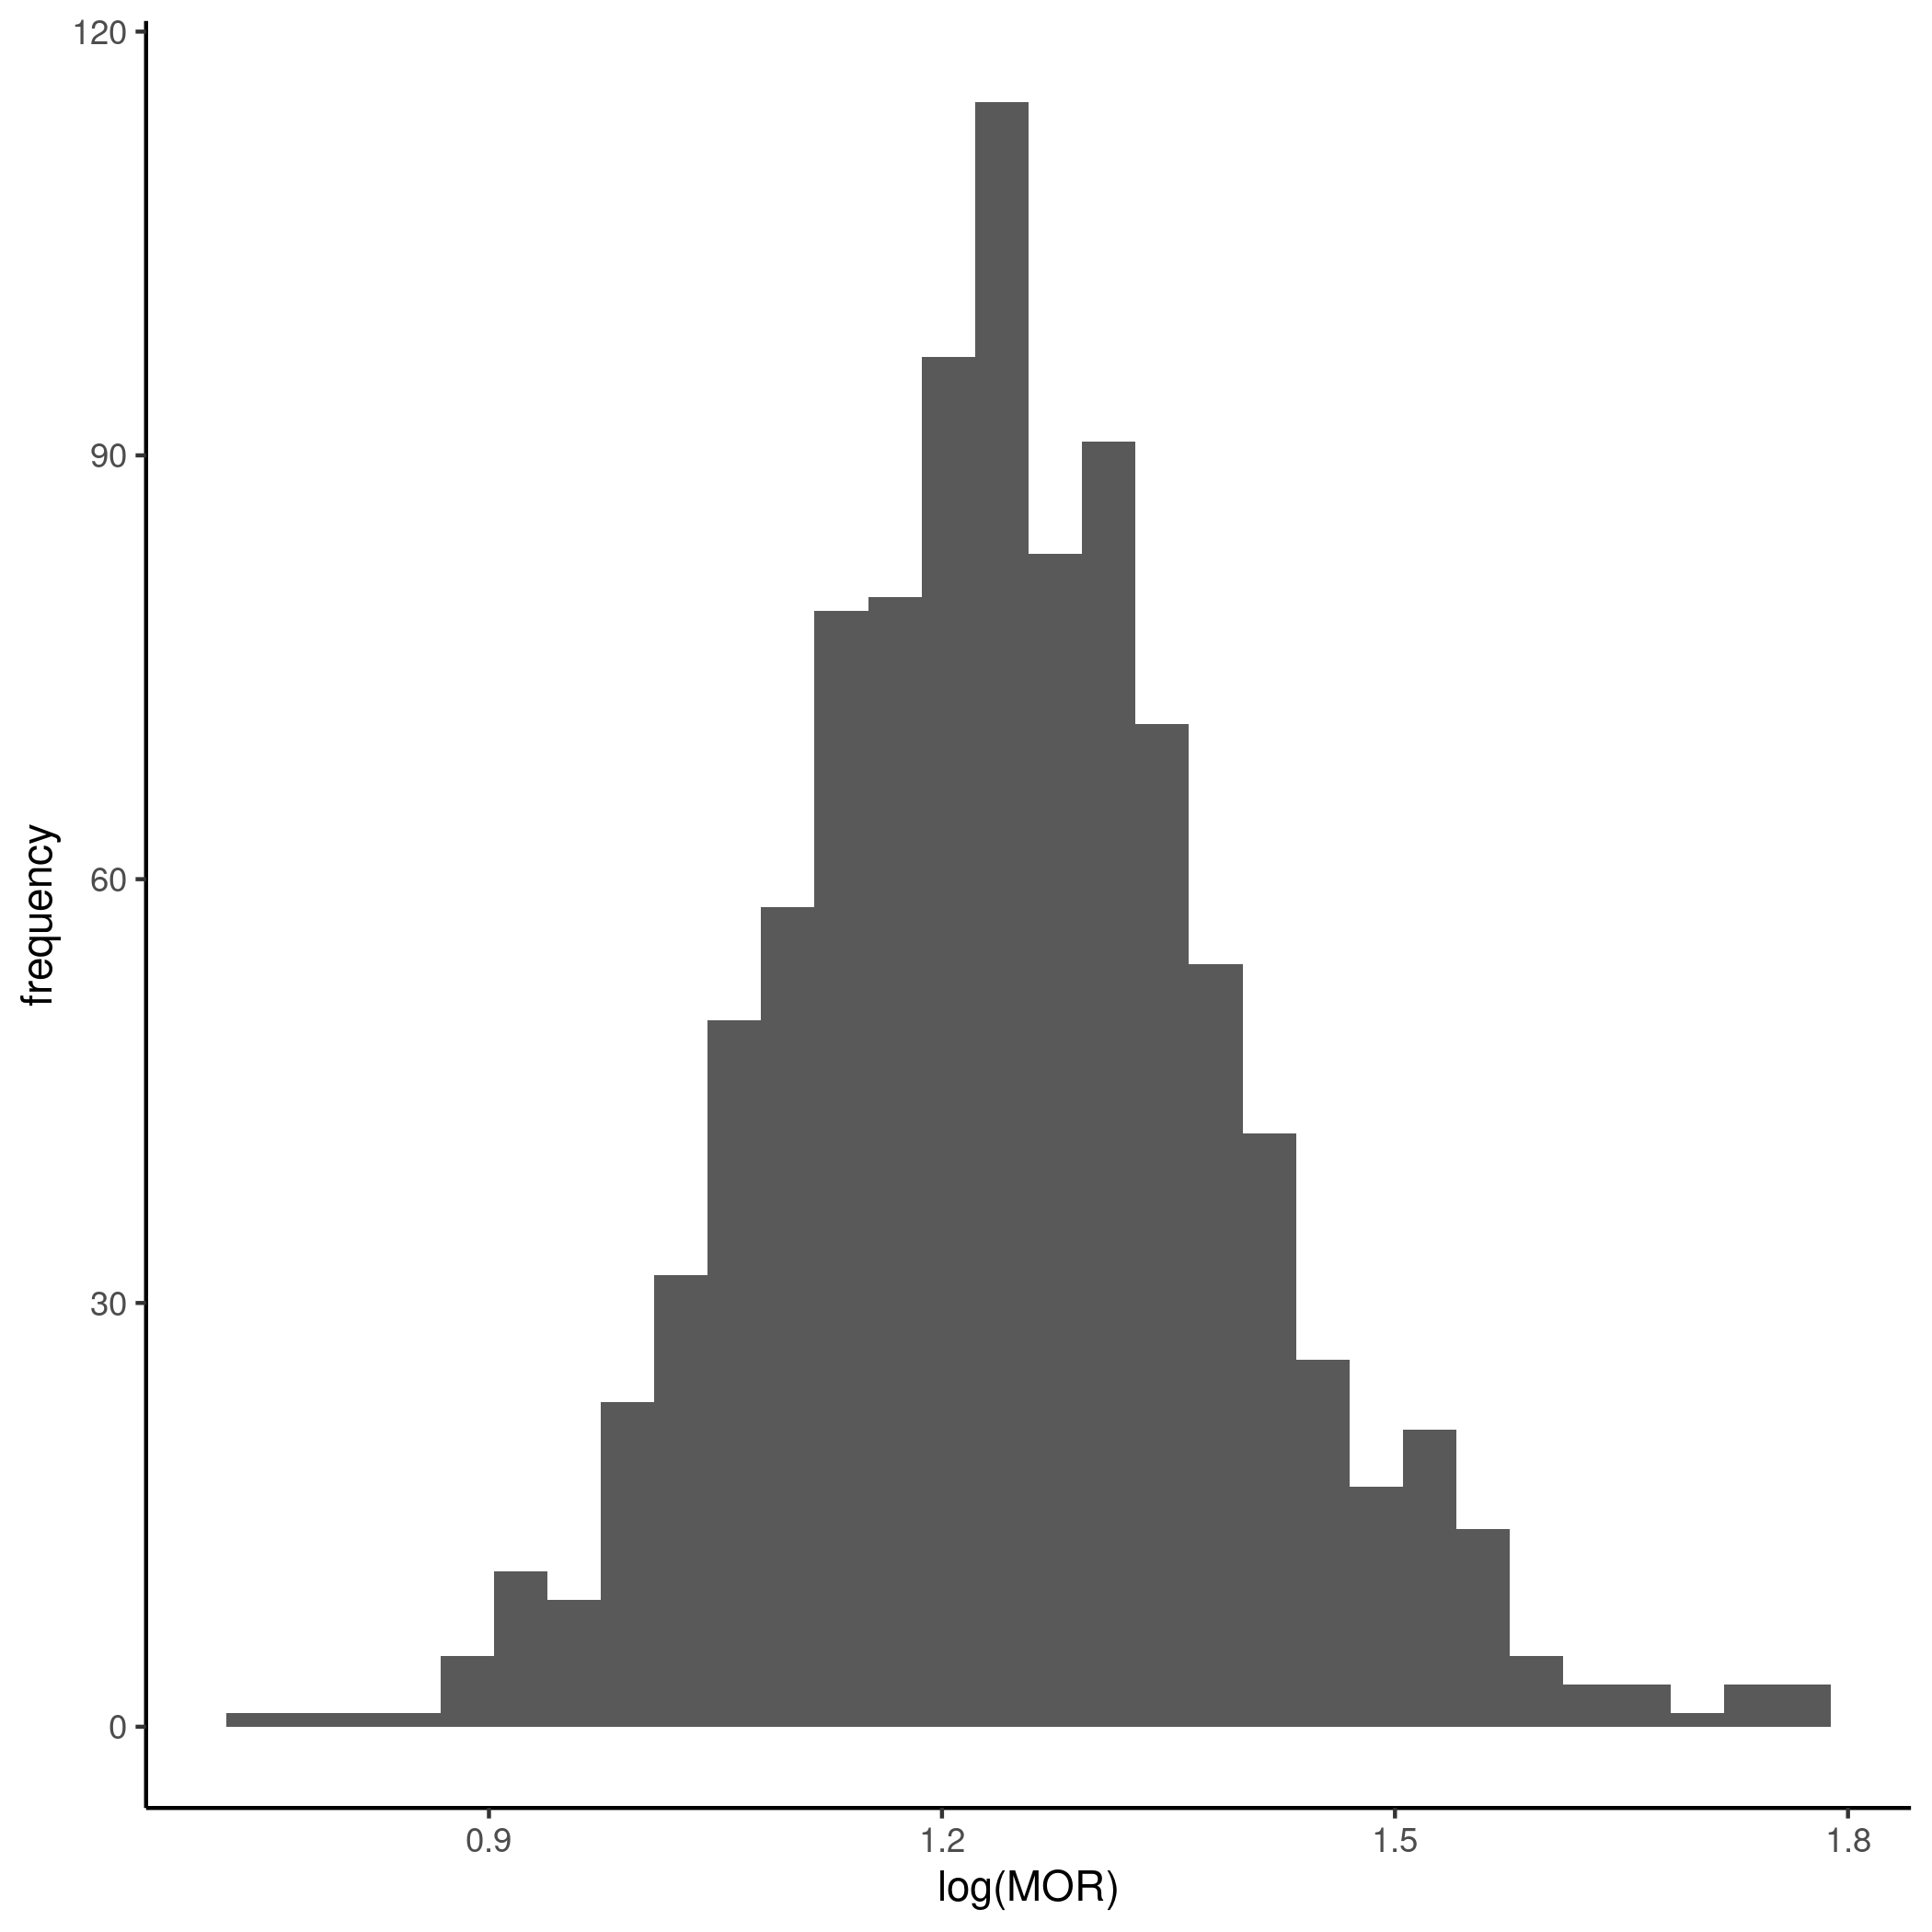
\includegraphics[width=.95\linewidth]{../../plots/three-lvl-ran-int/low-prev/hist_20_30_5_three_lvl_low_prev_mor1.png}  
    \caption{MOR\textsubscript{1}}
    \label{l20m30n51}
\end{subfigure}
\begin{subfigure}{.49\textwidth}
    \centering
    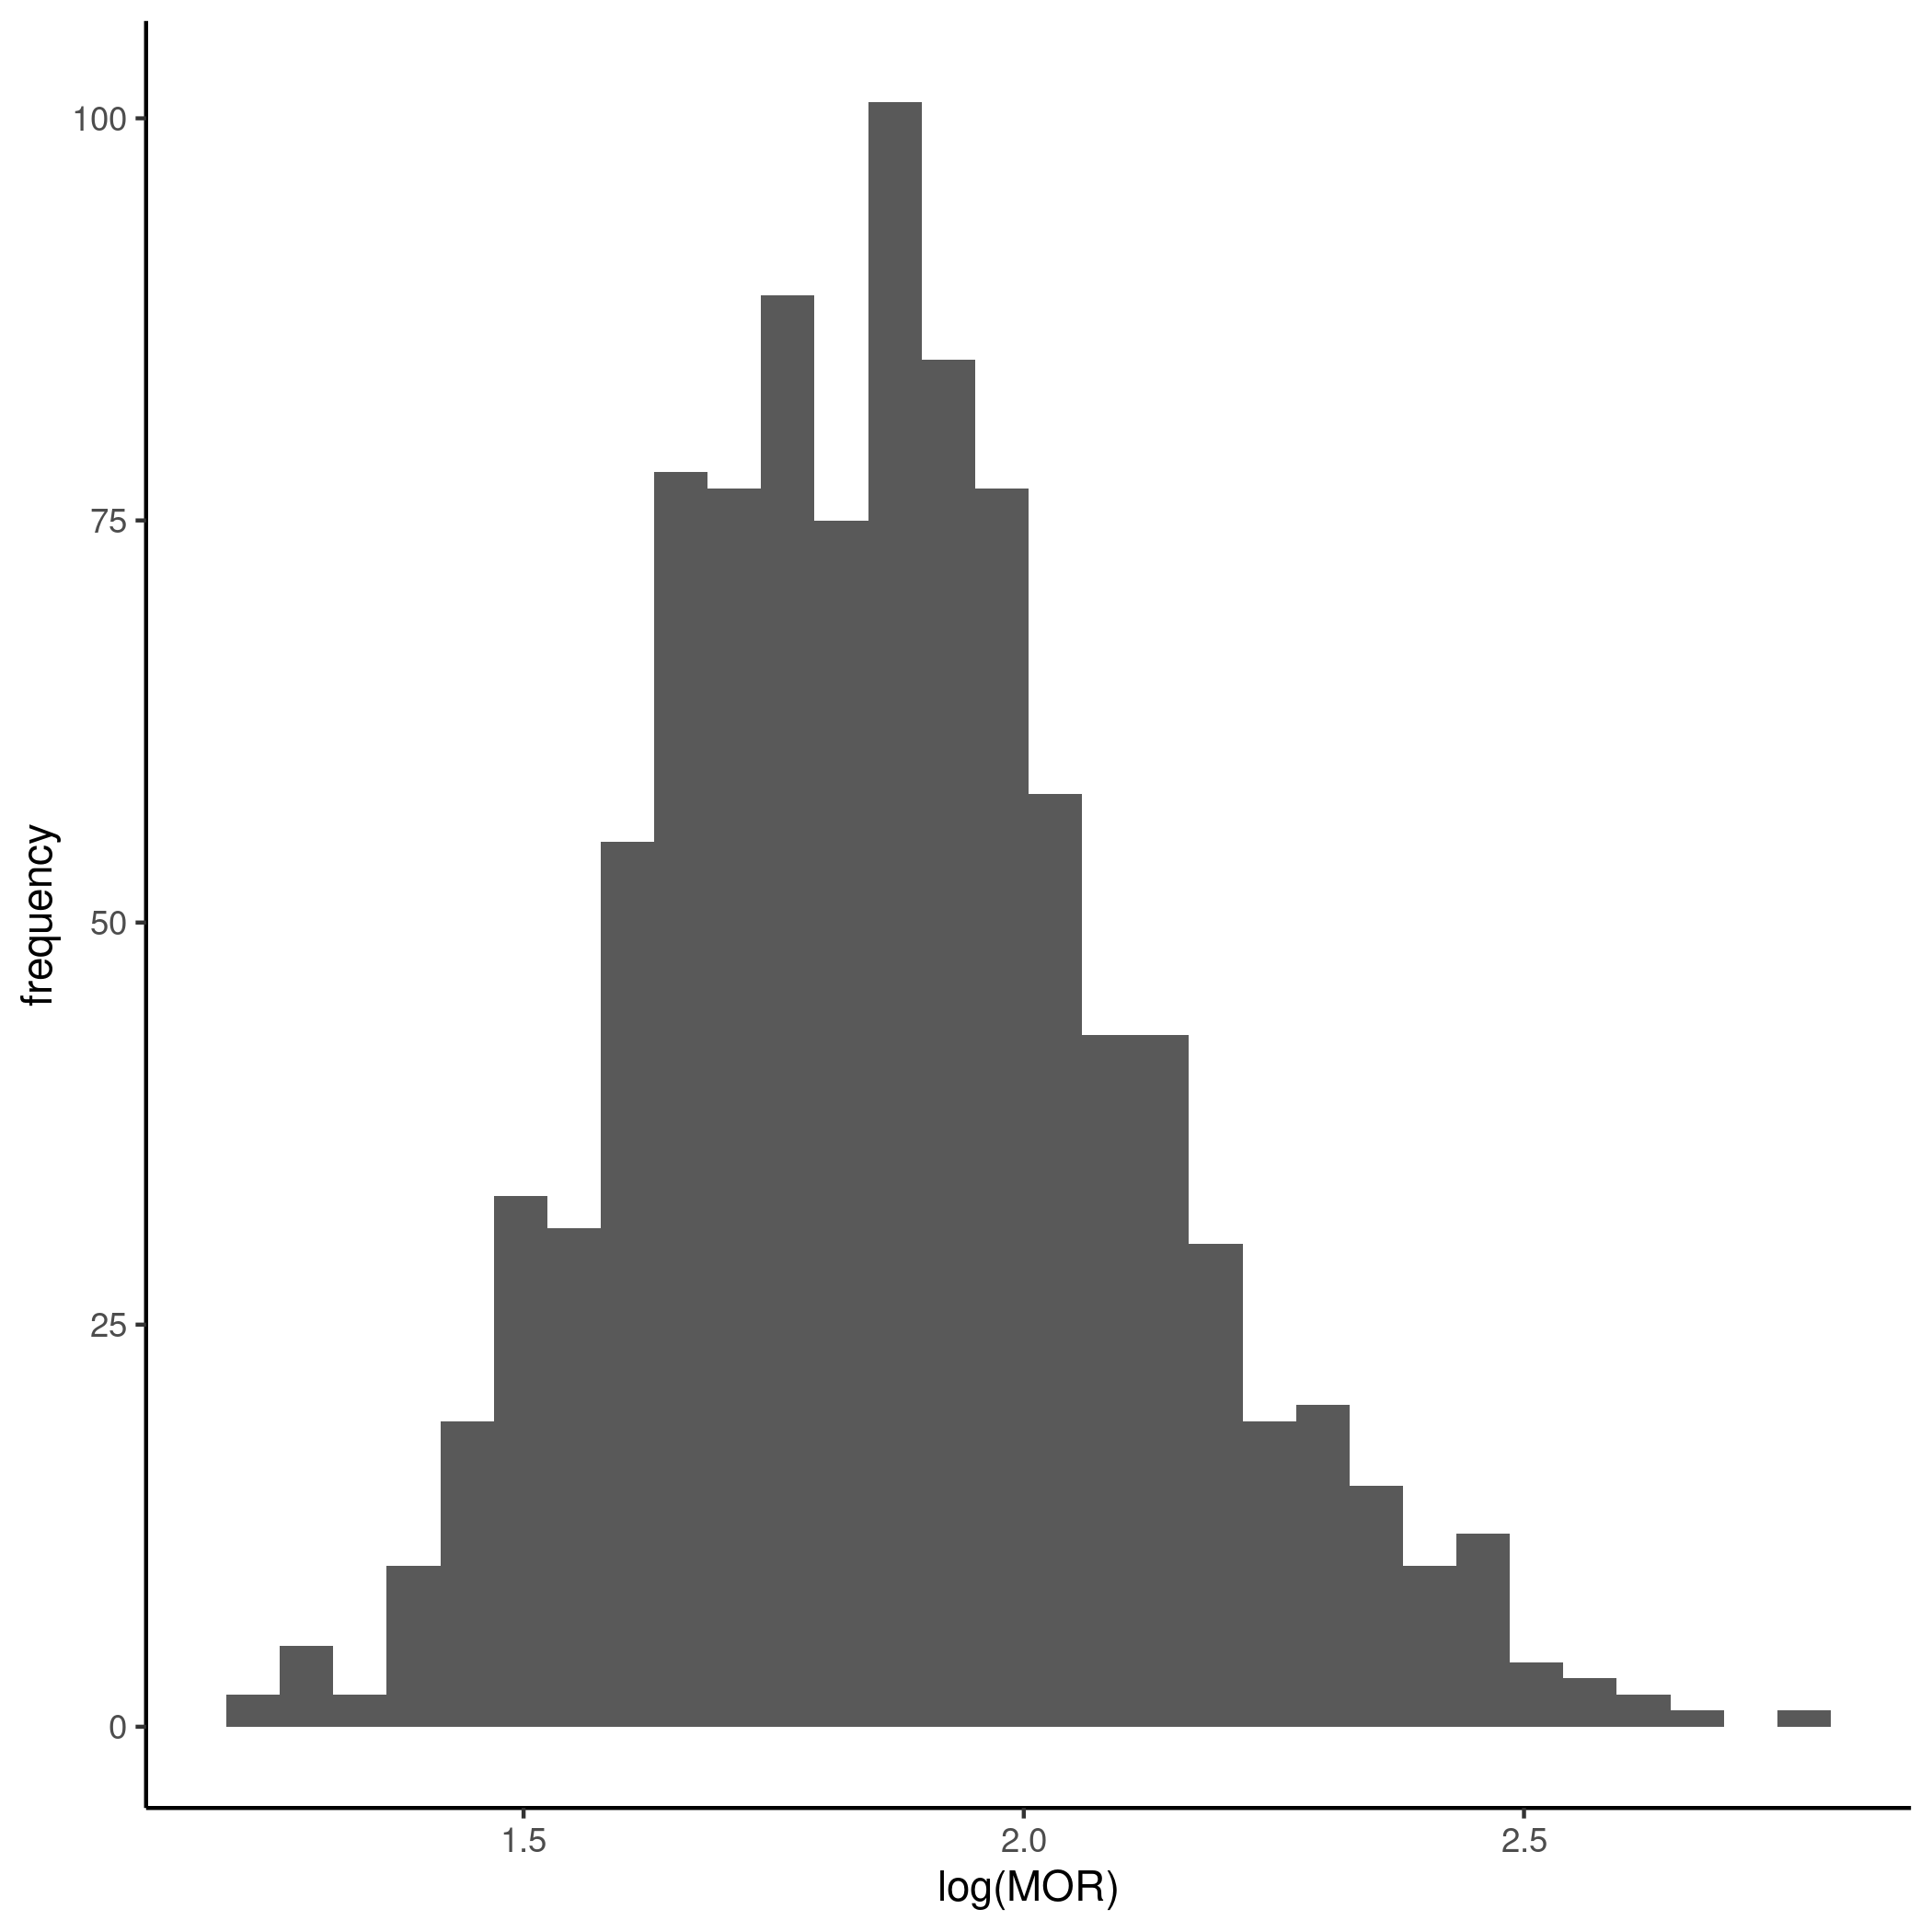
\includegraphics[width=.95\linewidth]{../../plots/three-lvl-ran-int/low-prev/hist_20_30_5_three_lvl_low_prev_mor2.png}  
    \caption{MOR\textsubscript{2}}
    \label{l20m30n52}
\end{subfigure}
\caption{Hospitals = 20, Doctors = 30, Patients = 5}
\label{mor1}
\end{figure}

\vspace{10mm}

\begin{figure}
\centering
\begin{subfigure}{.49\textwidth}
    \centering
    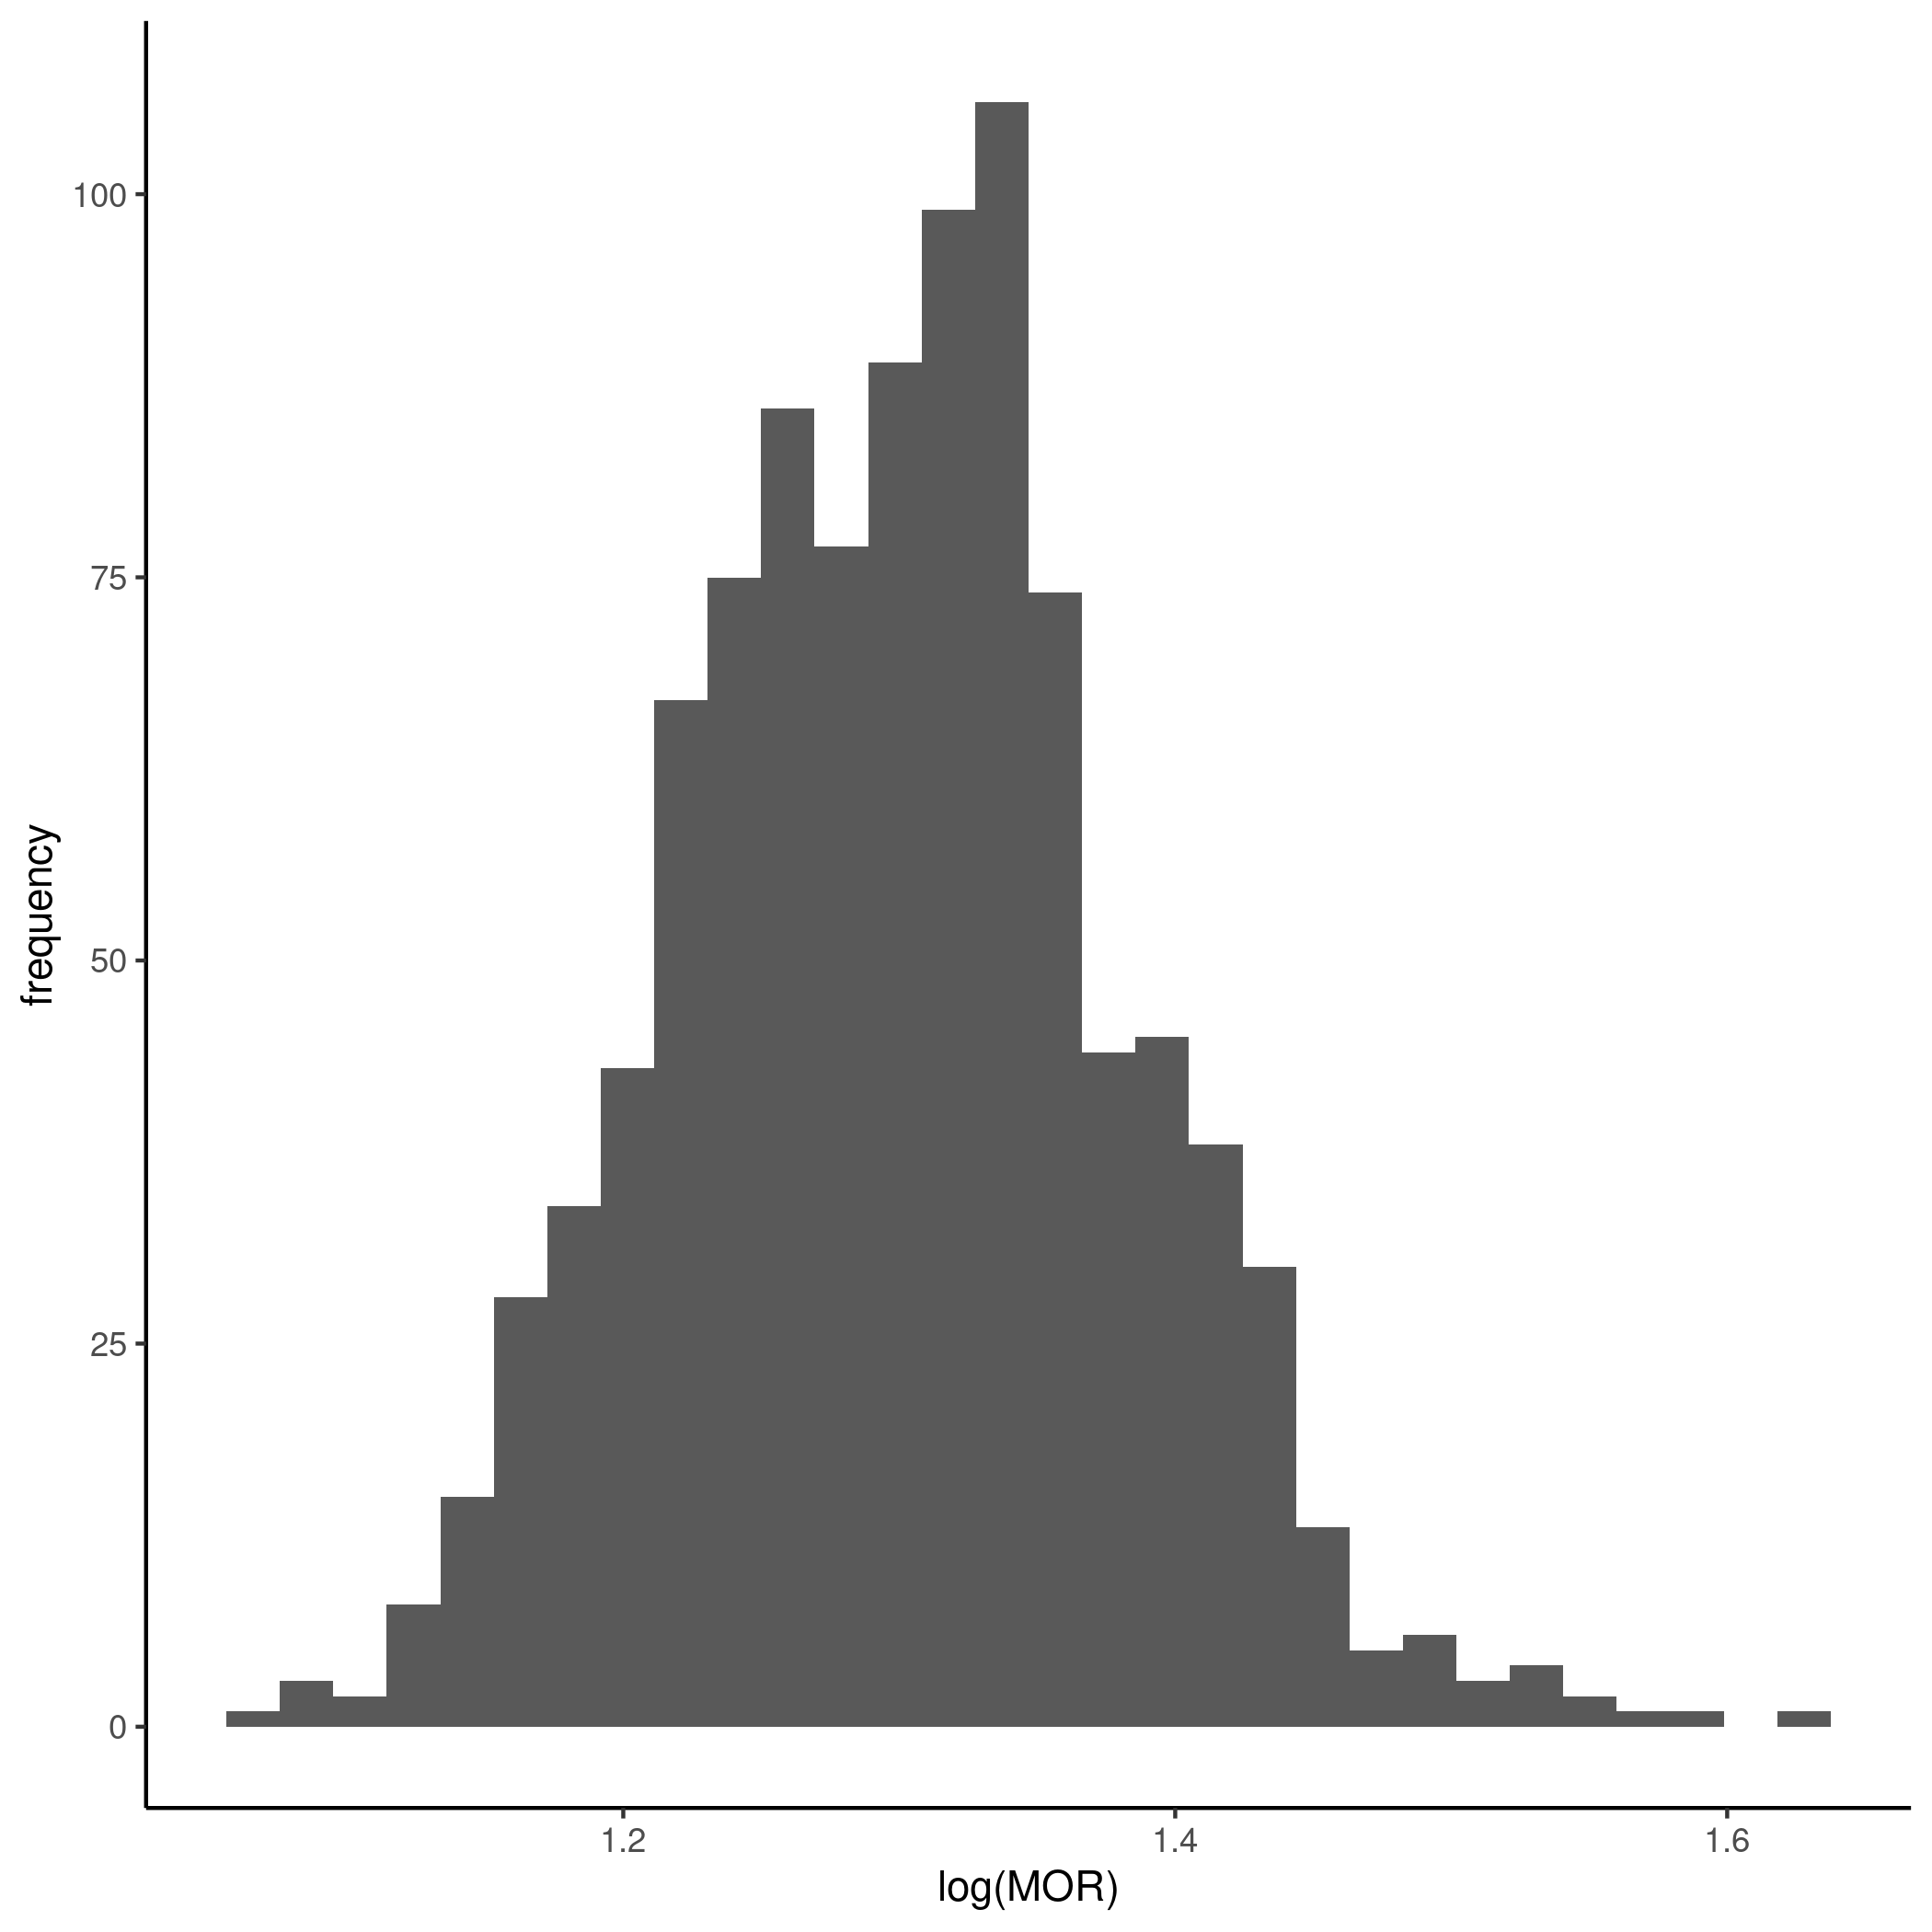
\includegraphics[width=.95\linewidth]{../../plots/three-lvl-ran-int/low-prev/hist_20_30_15_three_lvl_low_prev_mor1.png}  
    \caption{MOR\textsubscript{1}}
    \label{l20m30n151}
\end{subfigure}
\begin{subfigure}{.49\textwidth}
    \centering
    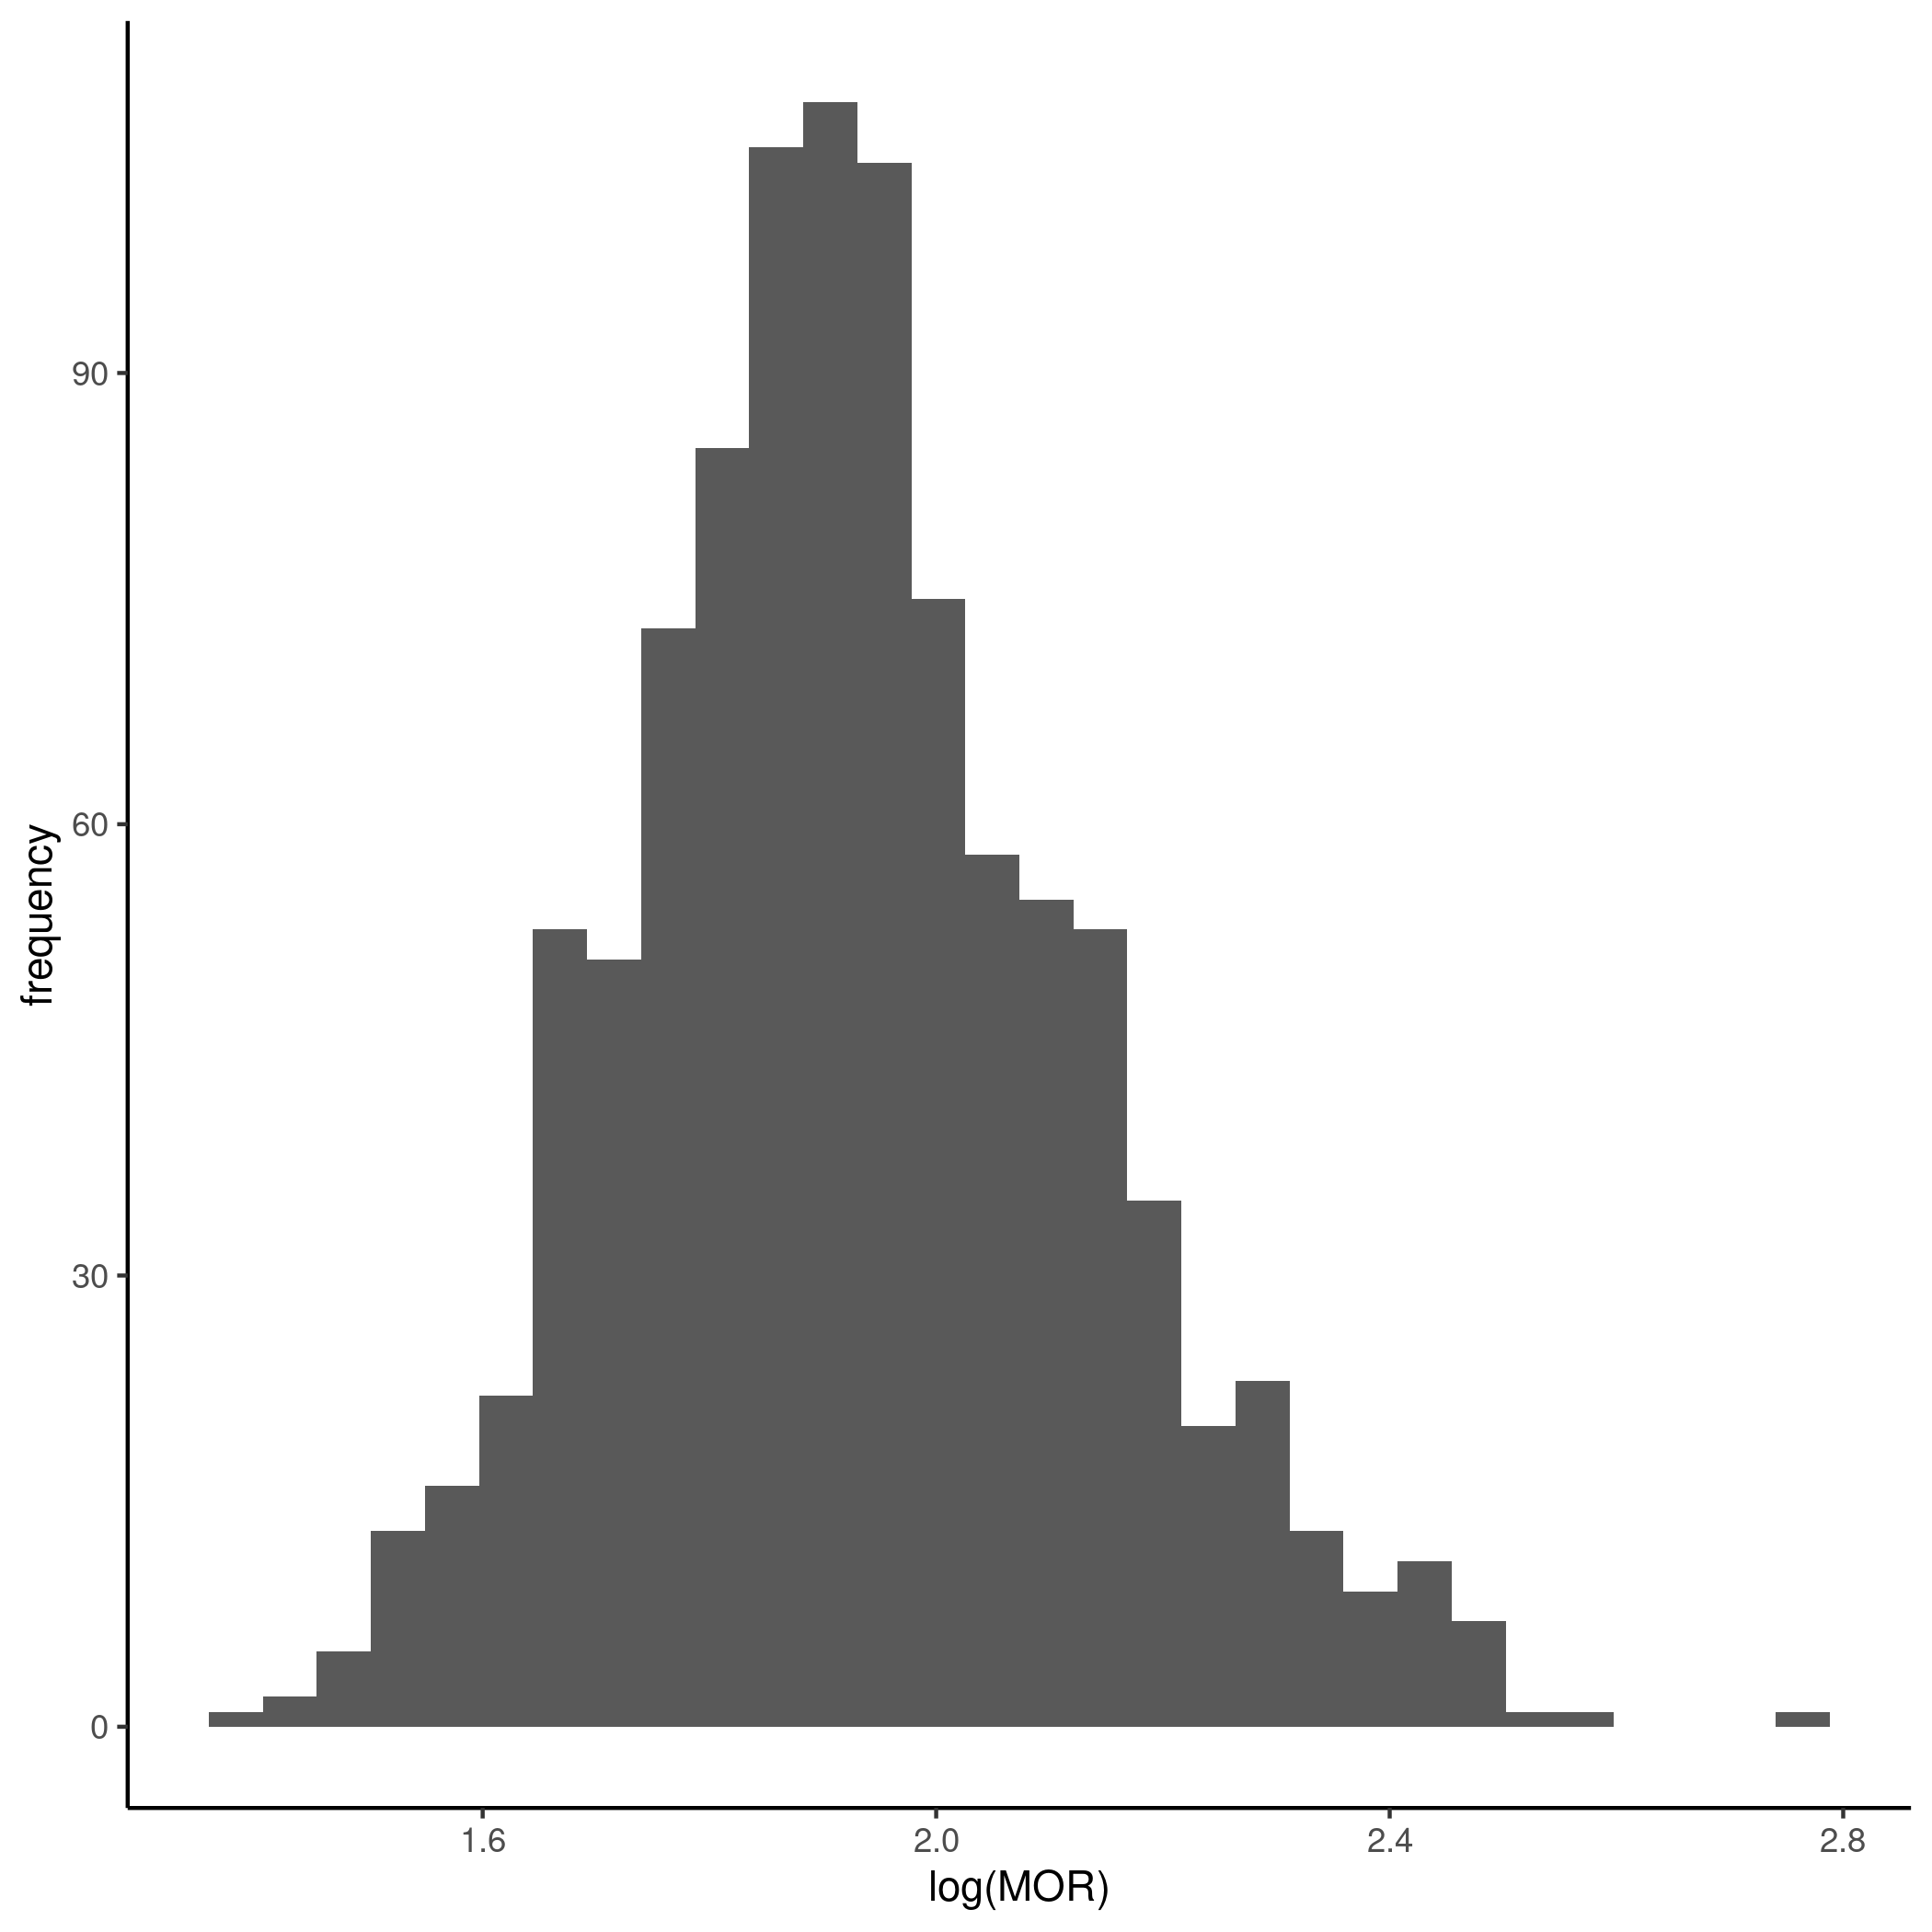
\includegraphics[width=.95\linewidth]{../../plots/three-lvl-ran-int/low-prev/hist_20_30_15_three_lvl_low_prev_mor2.png}
    \caption{MOR\textsubscript{2}}
    \label{l20m30n152}
\end{subfigure}
\caption{Hospitals = 20, Doctors = 30, Patients = 15}
\label{mor2}
\end{figure}

\vspace{10mm}

\begin{figure}
\centering
\begin{subfigure}{.49\textwidth}
    \centering
    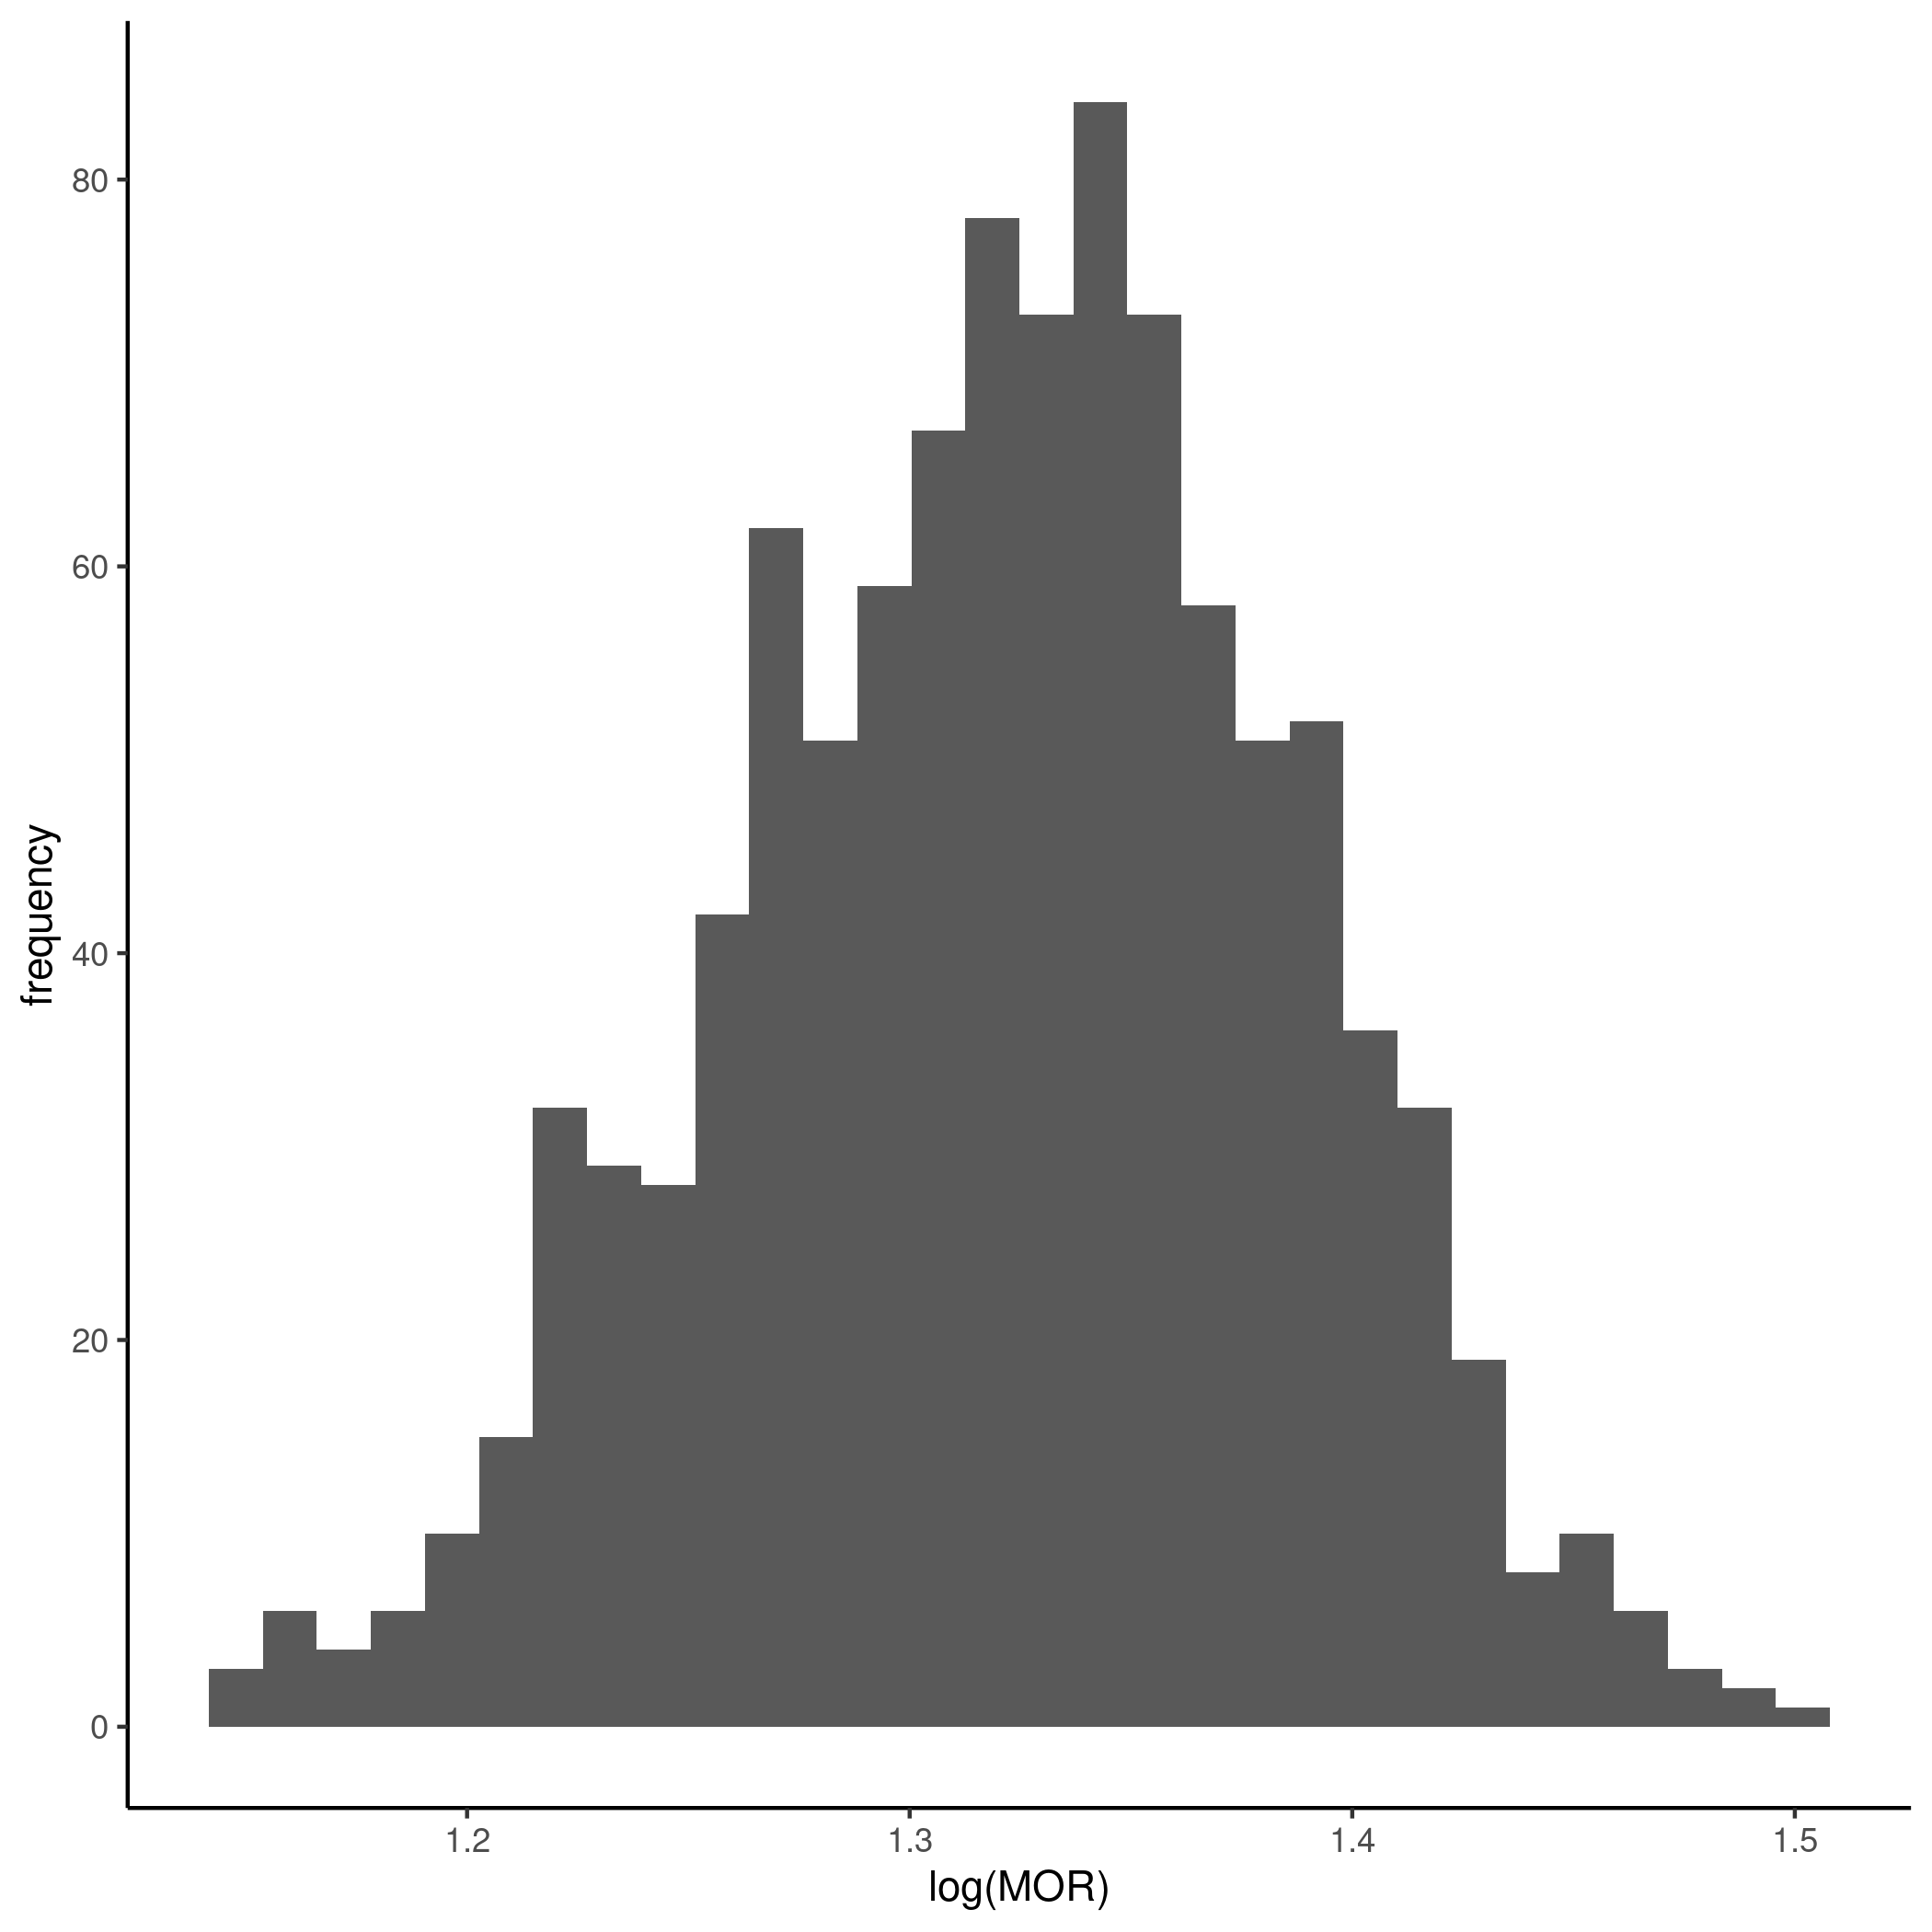
\includegraphics[width=.95\linewidth]{../../plots/three-lvl-ran-int/low-prev/hist_20_30_30_three_lvl_low_prev_mor1.png}  
    \caption{MOR\textsubscript{1}}
    \label{l20m30n301}
\end{subfigure}
\begin{subfigure}{.49\textwidth}
    \centering
    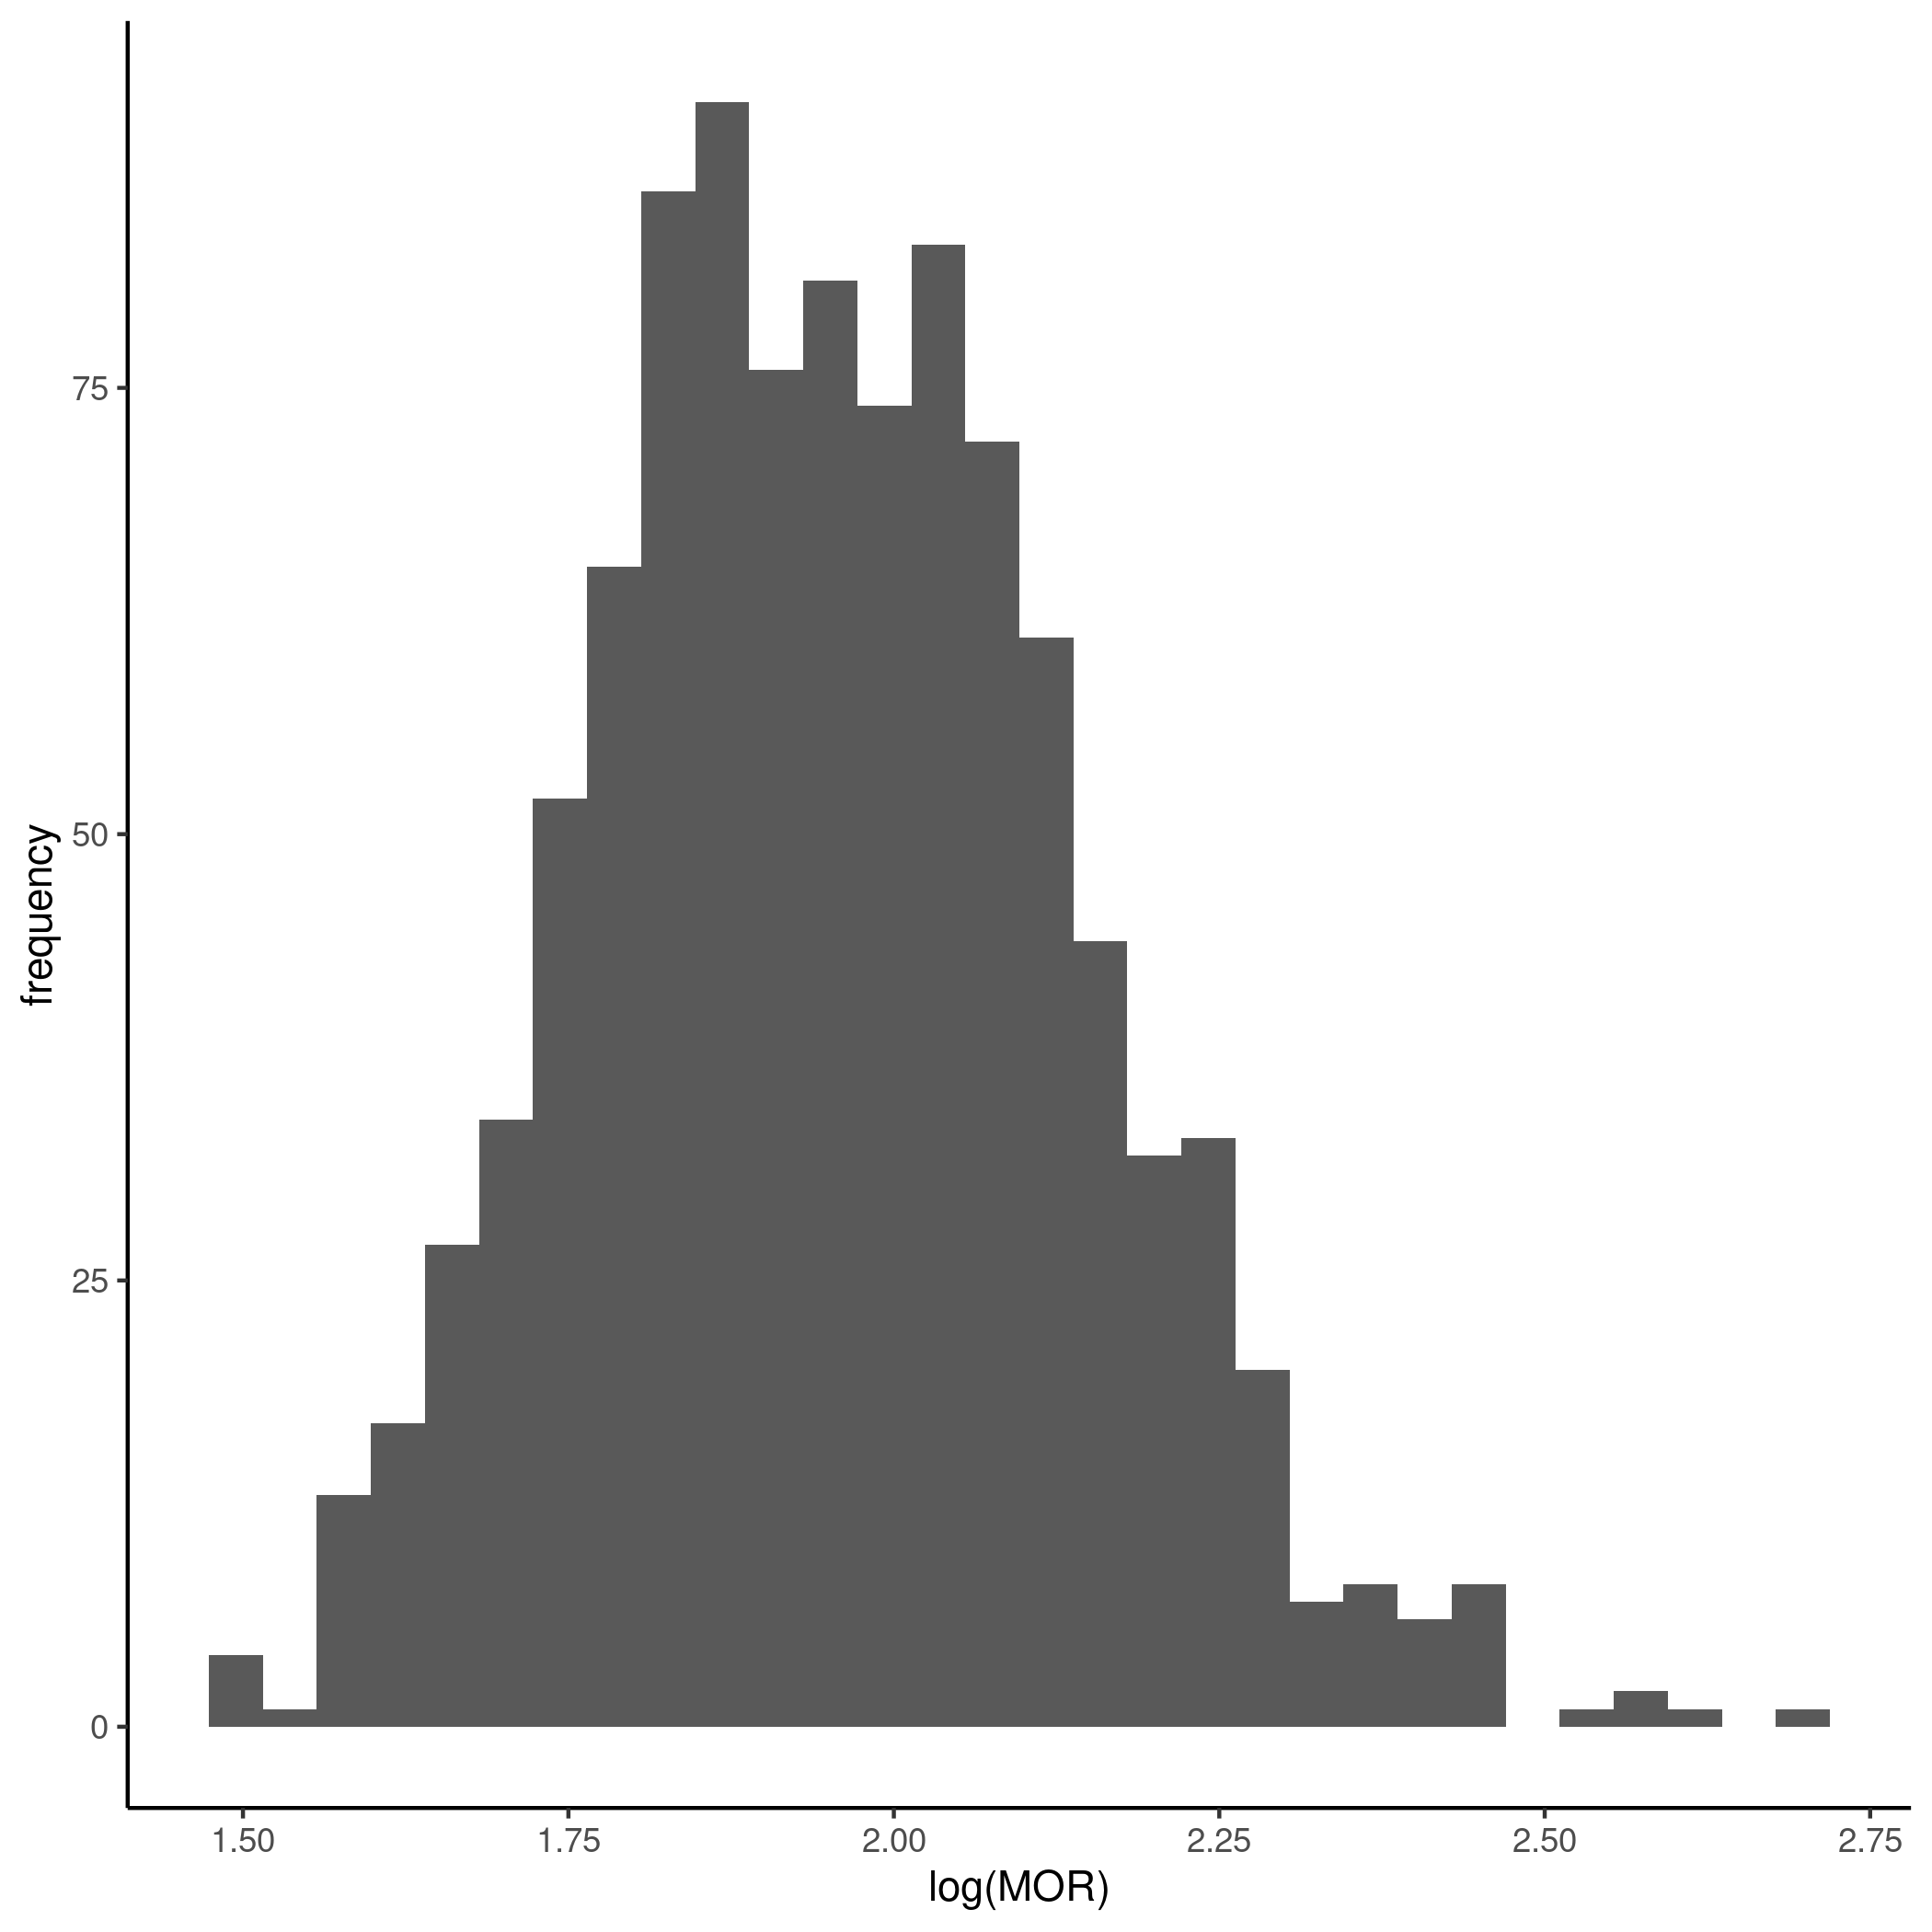
\includegraphics[width=.95\linewidth]{../../plots/three-lvl-ran-int/low-prev/hist_20_30_30_three_lvl_low_prev_mor2.png}
    \caption{MOR\textsubscript{2}}
    \label{l20m30n302}
\end{subfigure}
\caption{Hospitals = 20, Doctors = 30, Patients = 30}
\label{mor2}
\end{figure}

\vspace{10mm}

\begin{figure}
\centering
\begin{subfigure}{.49\textwidth}
    \centering
    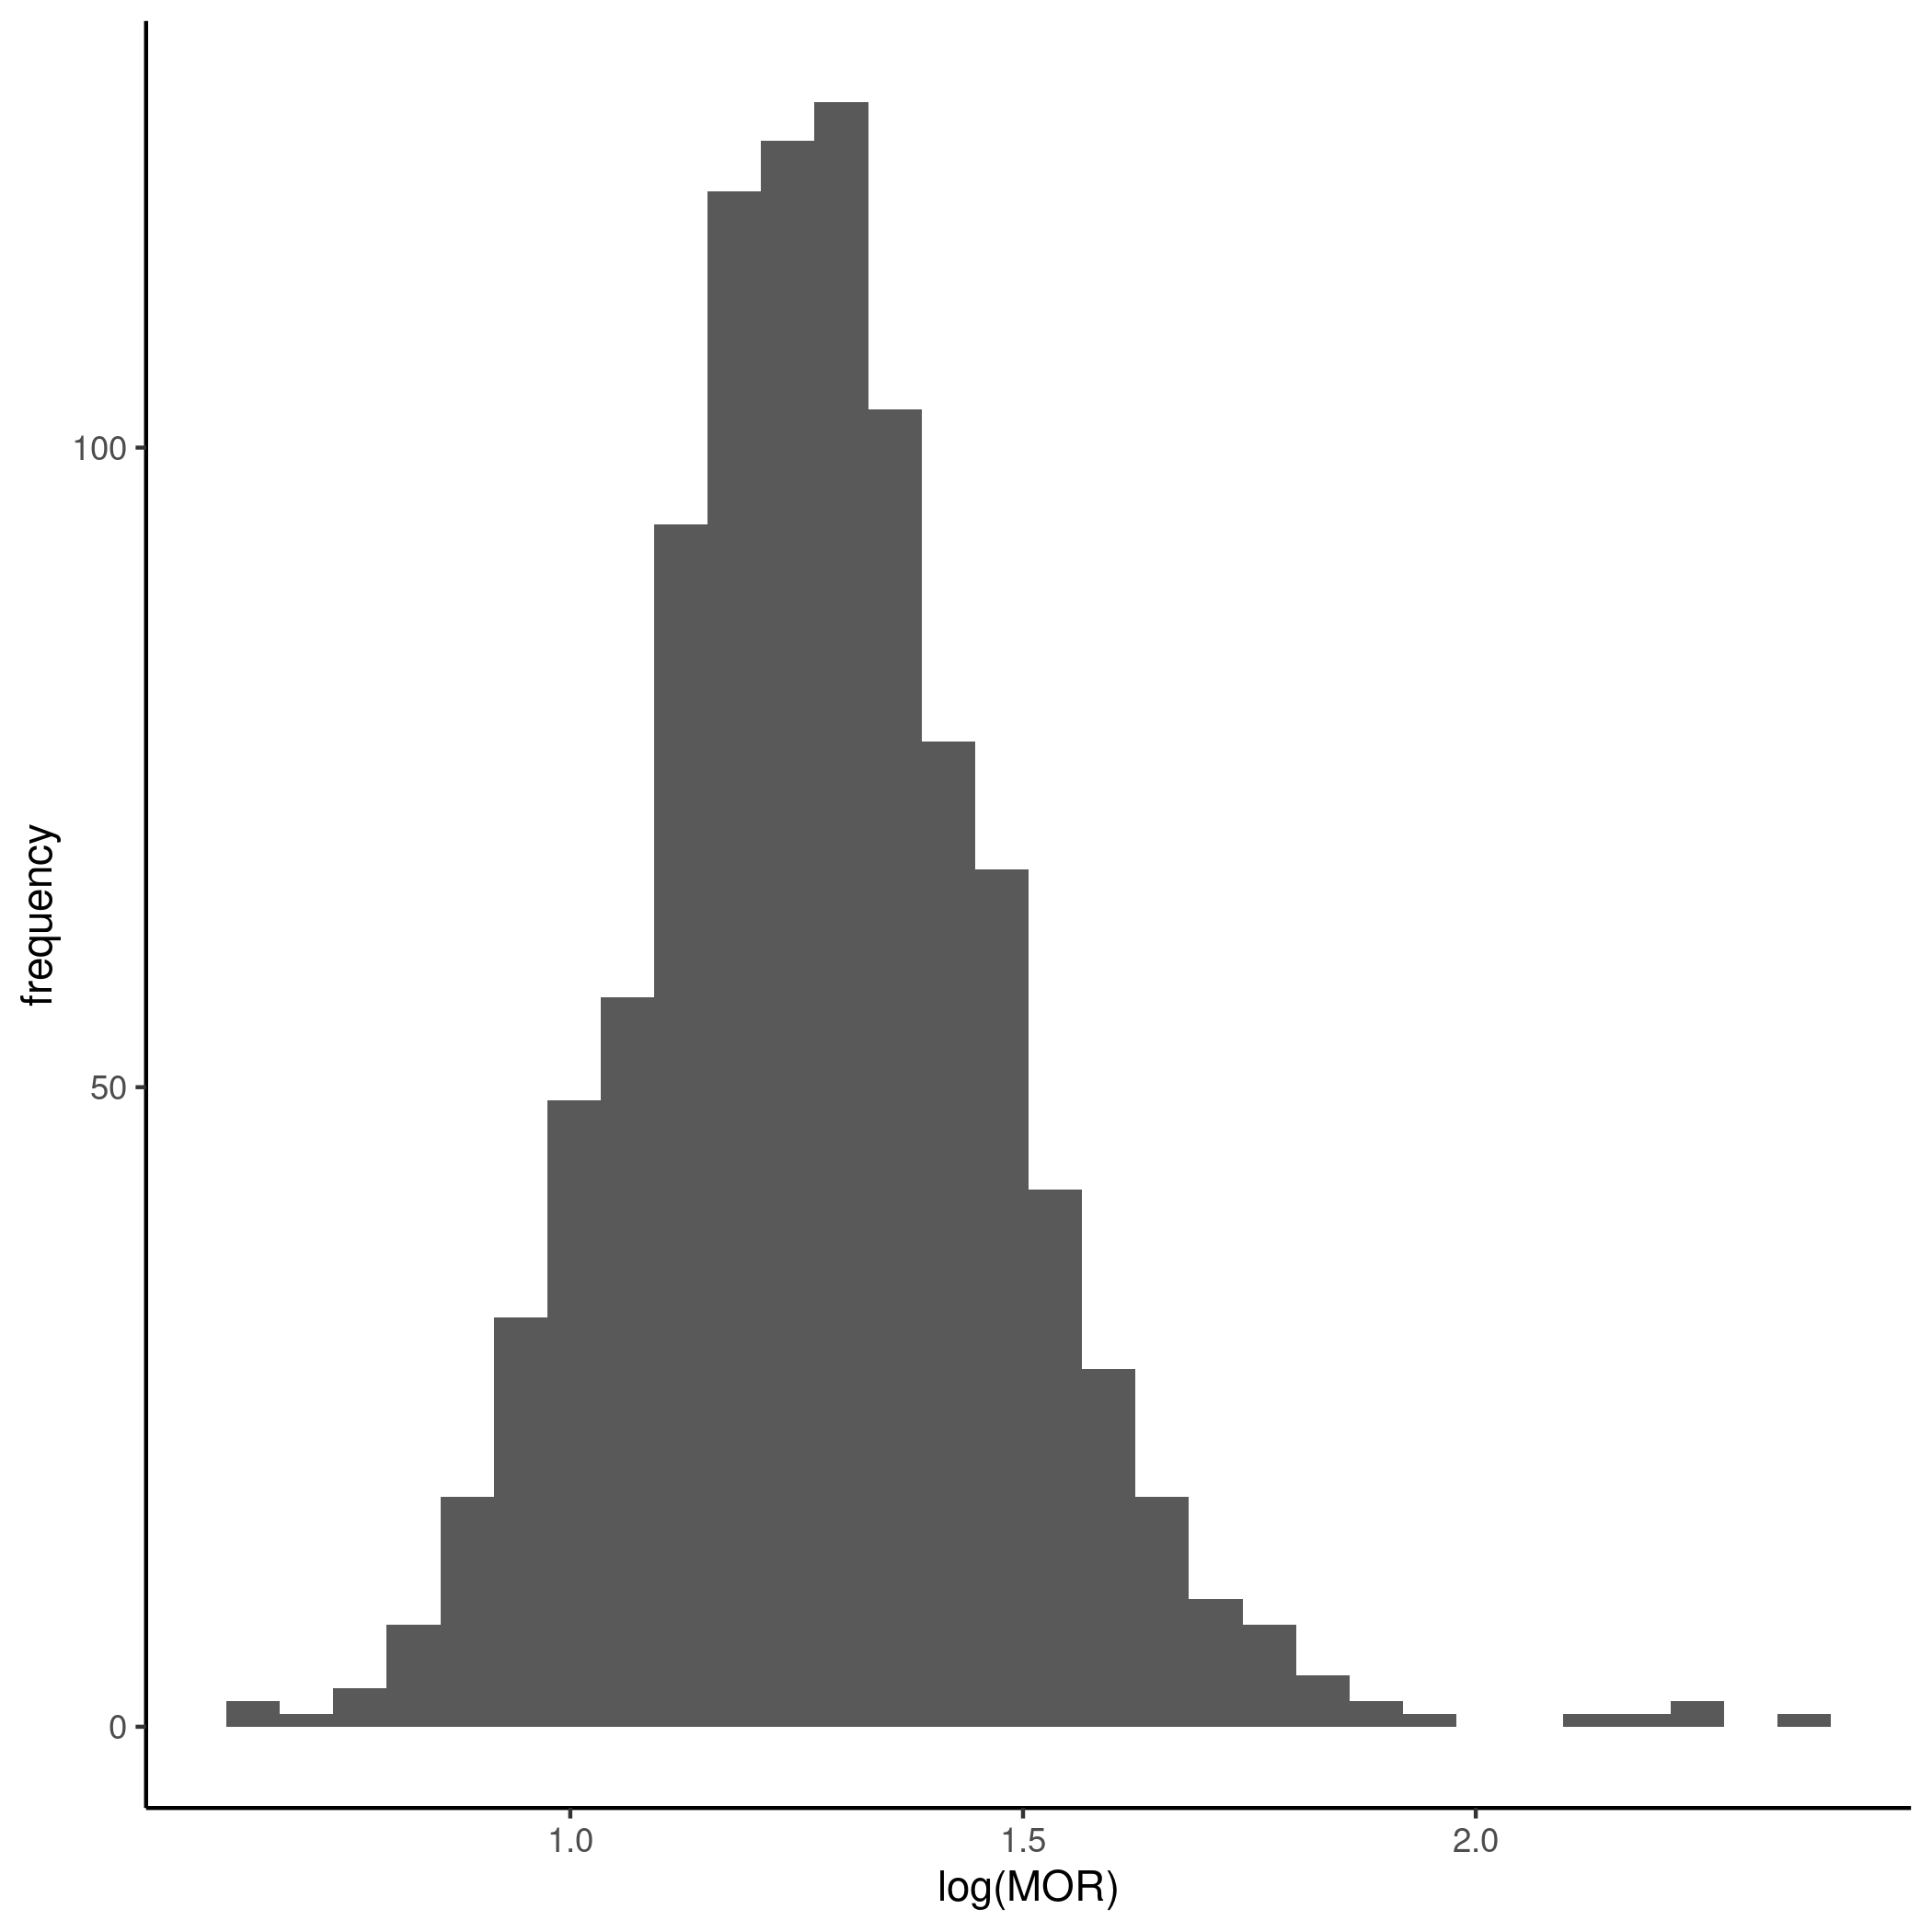
\includegraphics[width=.95\linewidth]{../../plots/three-lvl-ran-int/low-prev/hist_40_10_5_three_lvl_low_prev_mor1.png}  
    \caption{MOR\textsubscript{1}}
    \label{l40m10n51}
\end{subfigure}
\begin{subfigure}{.49\textwidth}
    \centering
    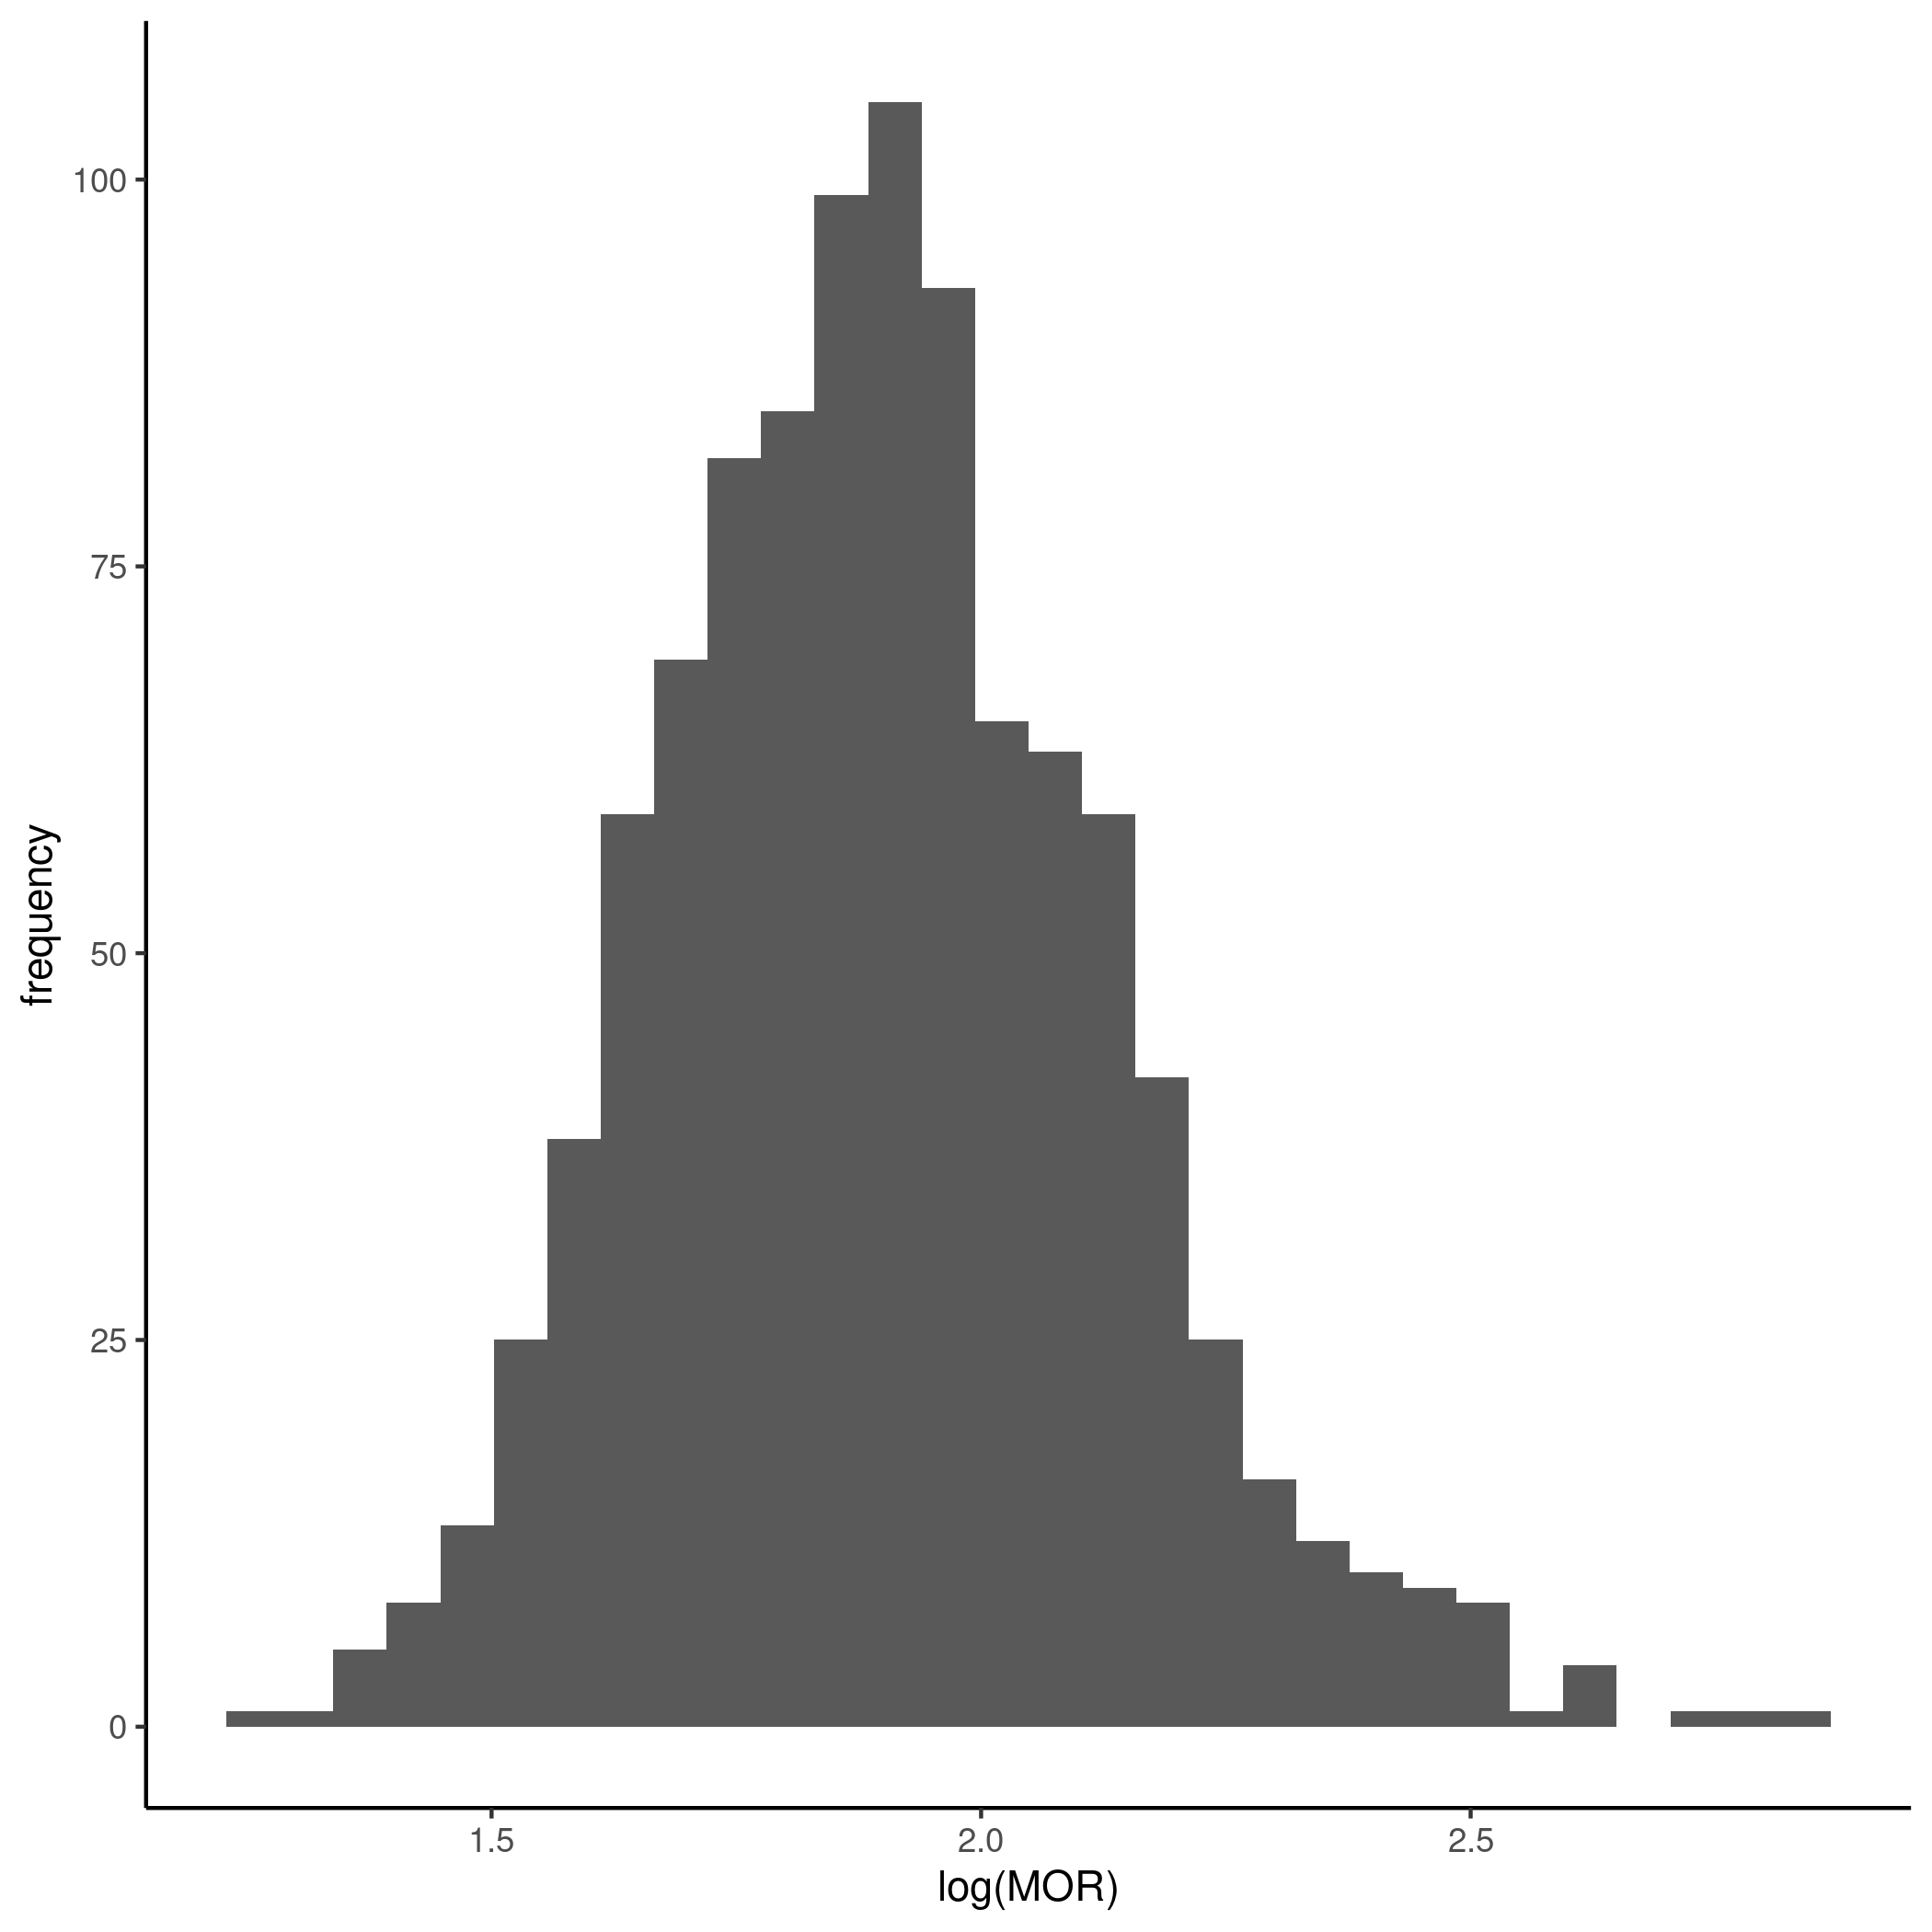
\includegraphics[width=.95\linewidth]{../../plots/three-lvl-ran-int/low-prev/hist_40_10_5_three_lvl_low_prev_mor2.png}
    \caption{MOR\textsubscript{2}}
    \label{l40m10n52}
\end{subfigure}
\caption{Hospitals = 40, Doctors = 10, Patients = 5}
\label{mor2}
\end{figure}

\vspace{10mm}

\begin{figure}
\centering
\begin{subfigure}{.49\textwidth}
    \centering
    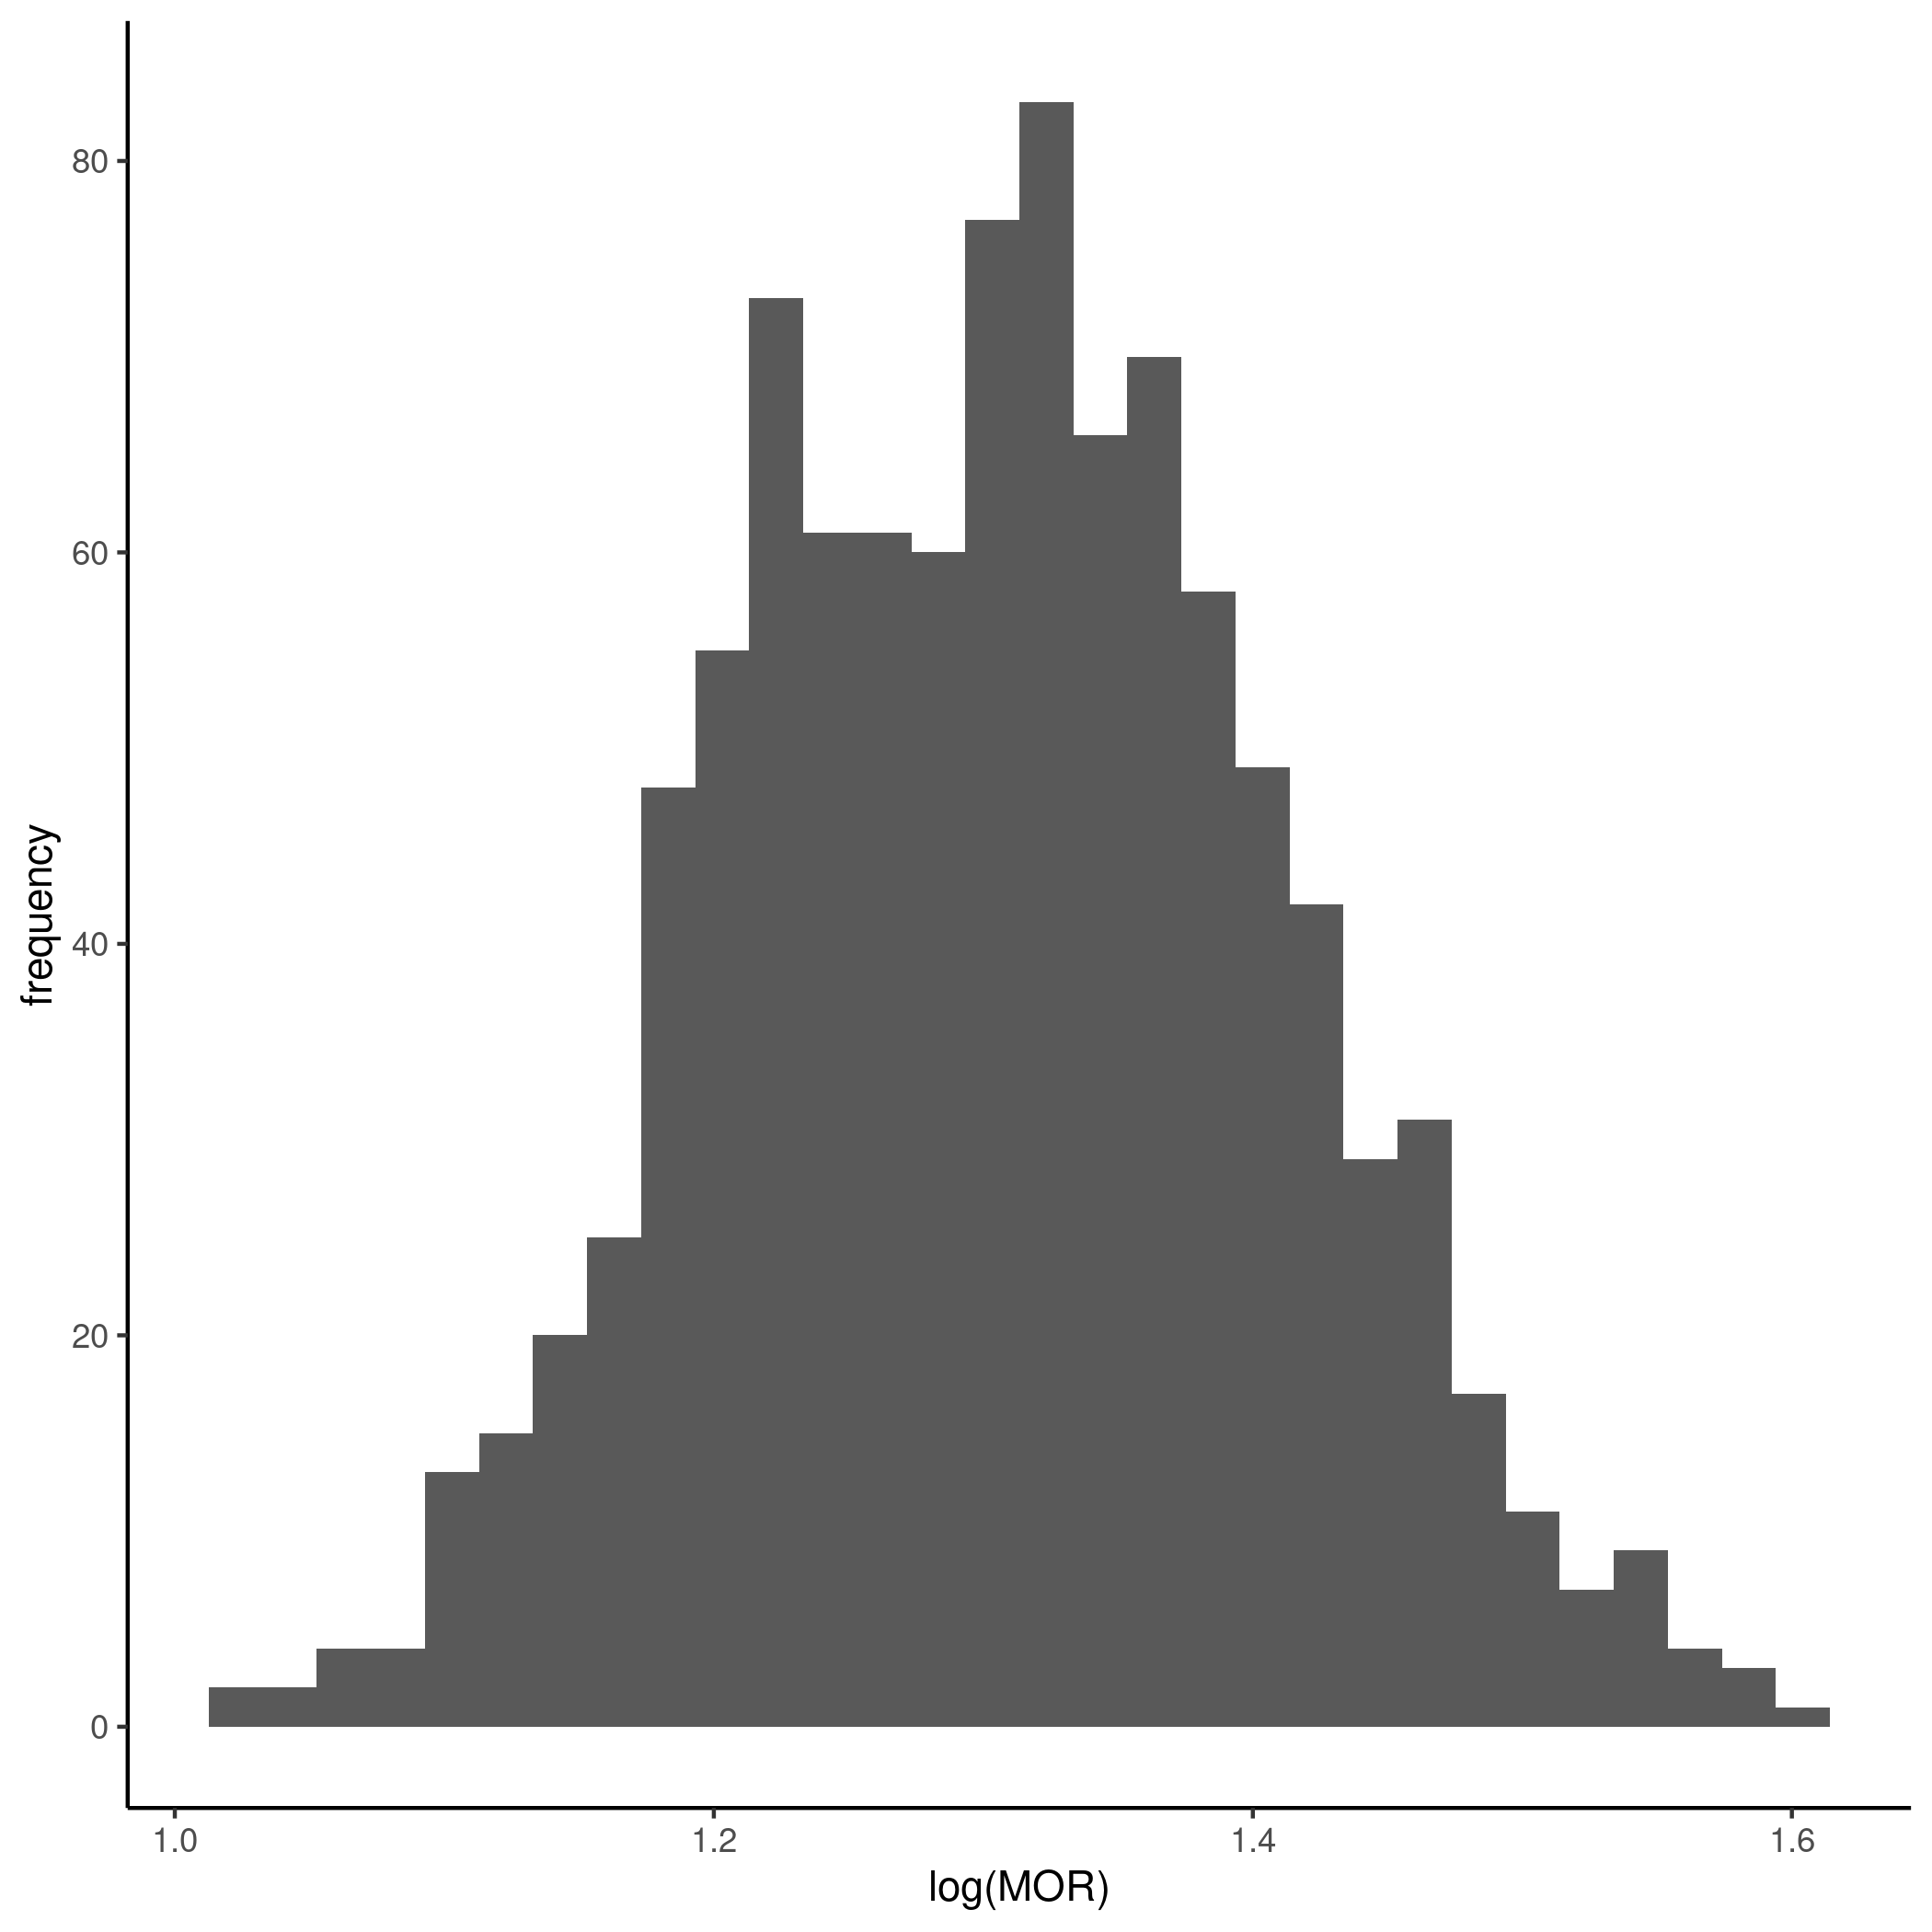
\includegraphics[width=.95\linewidth]{../../plots/three-lvl-ran-int/low-prev/hist_40_10_15_three_lvl_low_prev_mor1.png}  
    \caption{MOR\textsubscript{1}}
    \label{l40m10n151}
\end{subfigure}
\begin{subfigure}{.49\textwidth}
    \centering
    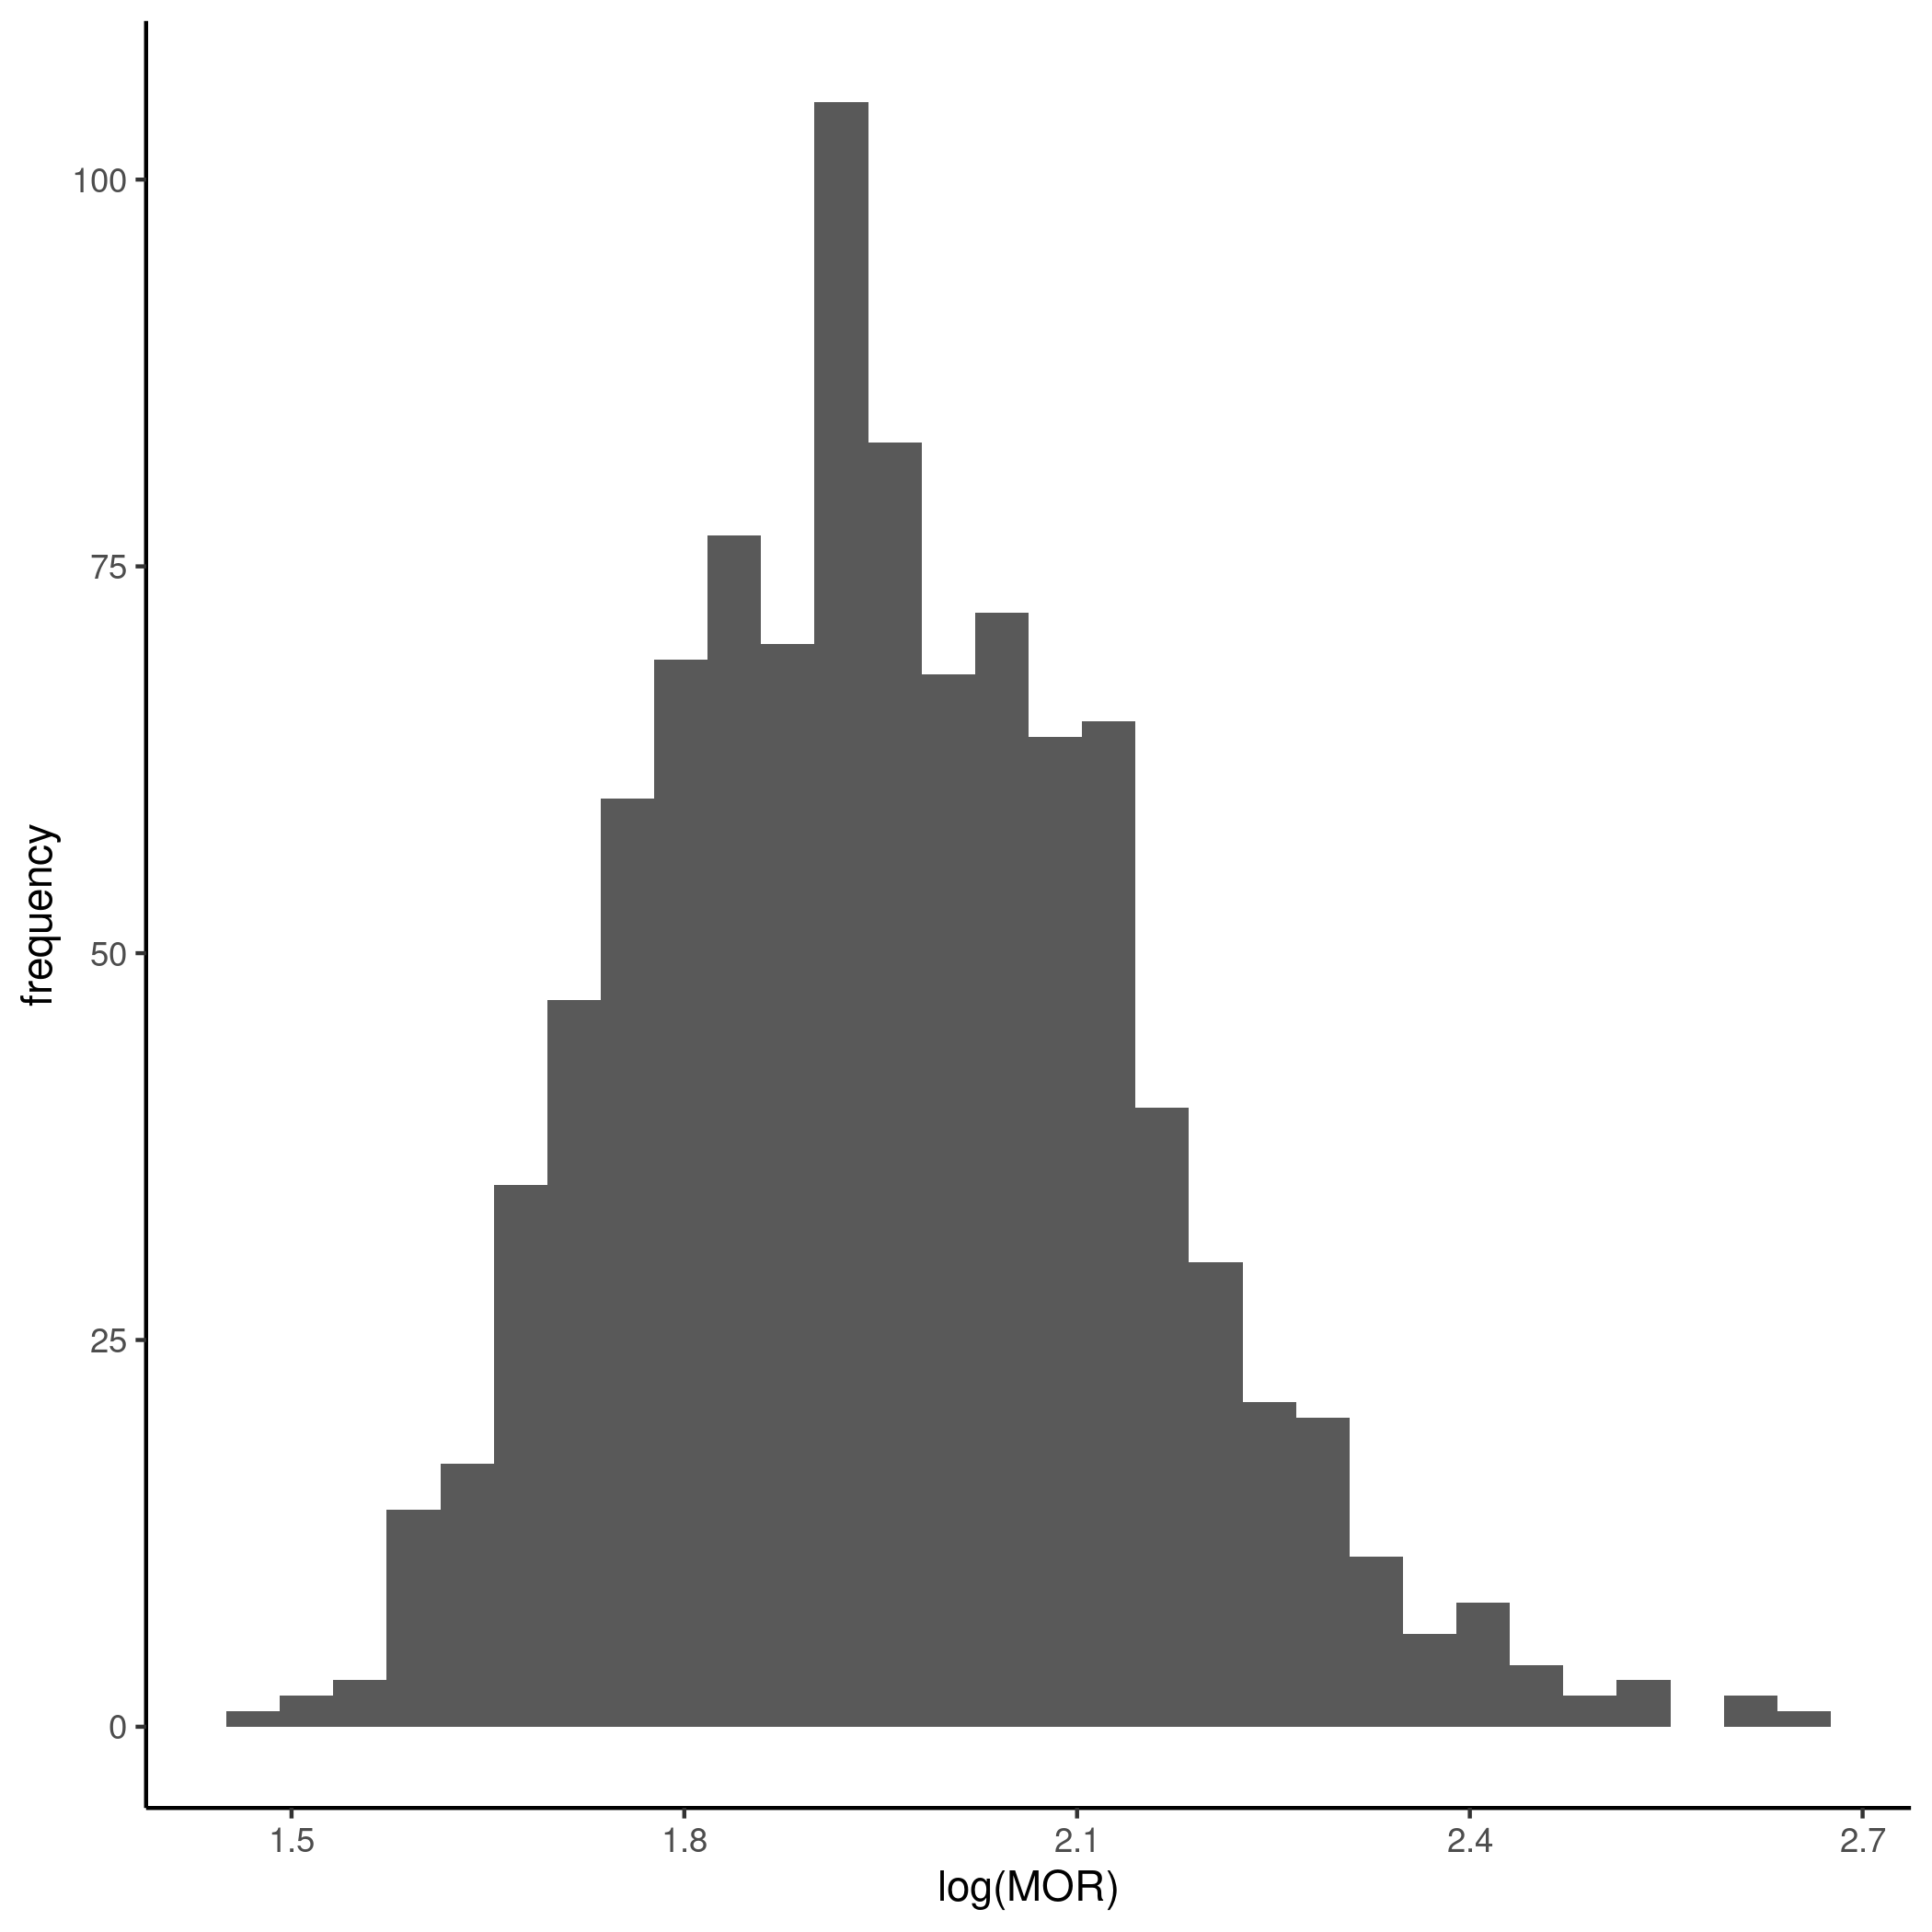
\includegraphics[width=.95\linewidth]{../../plots/three-lvl-ran-int/low-prev/hist_40_10_15_three_lvl_low_prev_mor2.png}
    \caption{MOR\textsubscript{2}}
    \label{l40m10n152}
\end{subfigure}
\caption{Hospitals = 40, Doctors = 10, Patients = 15}
\label{mor2}
\end{figure}

\vspace{10mm}

\begin{figure}
\centering
\begin{subfigure}{.49\textwidth}
    \centering
    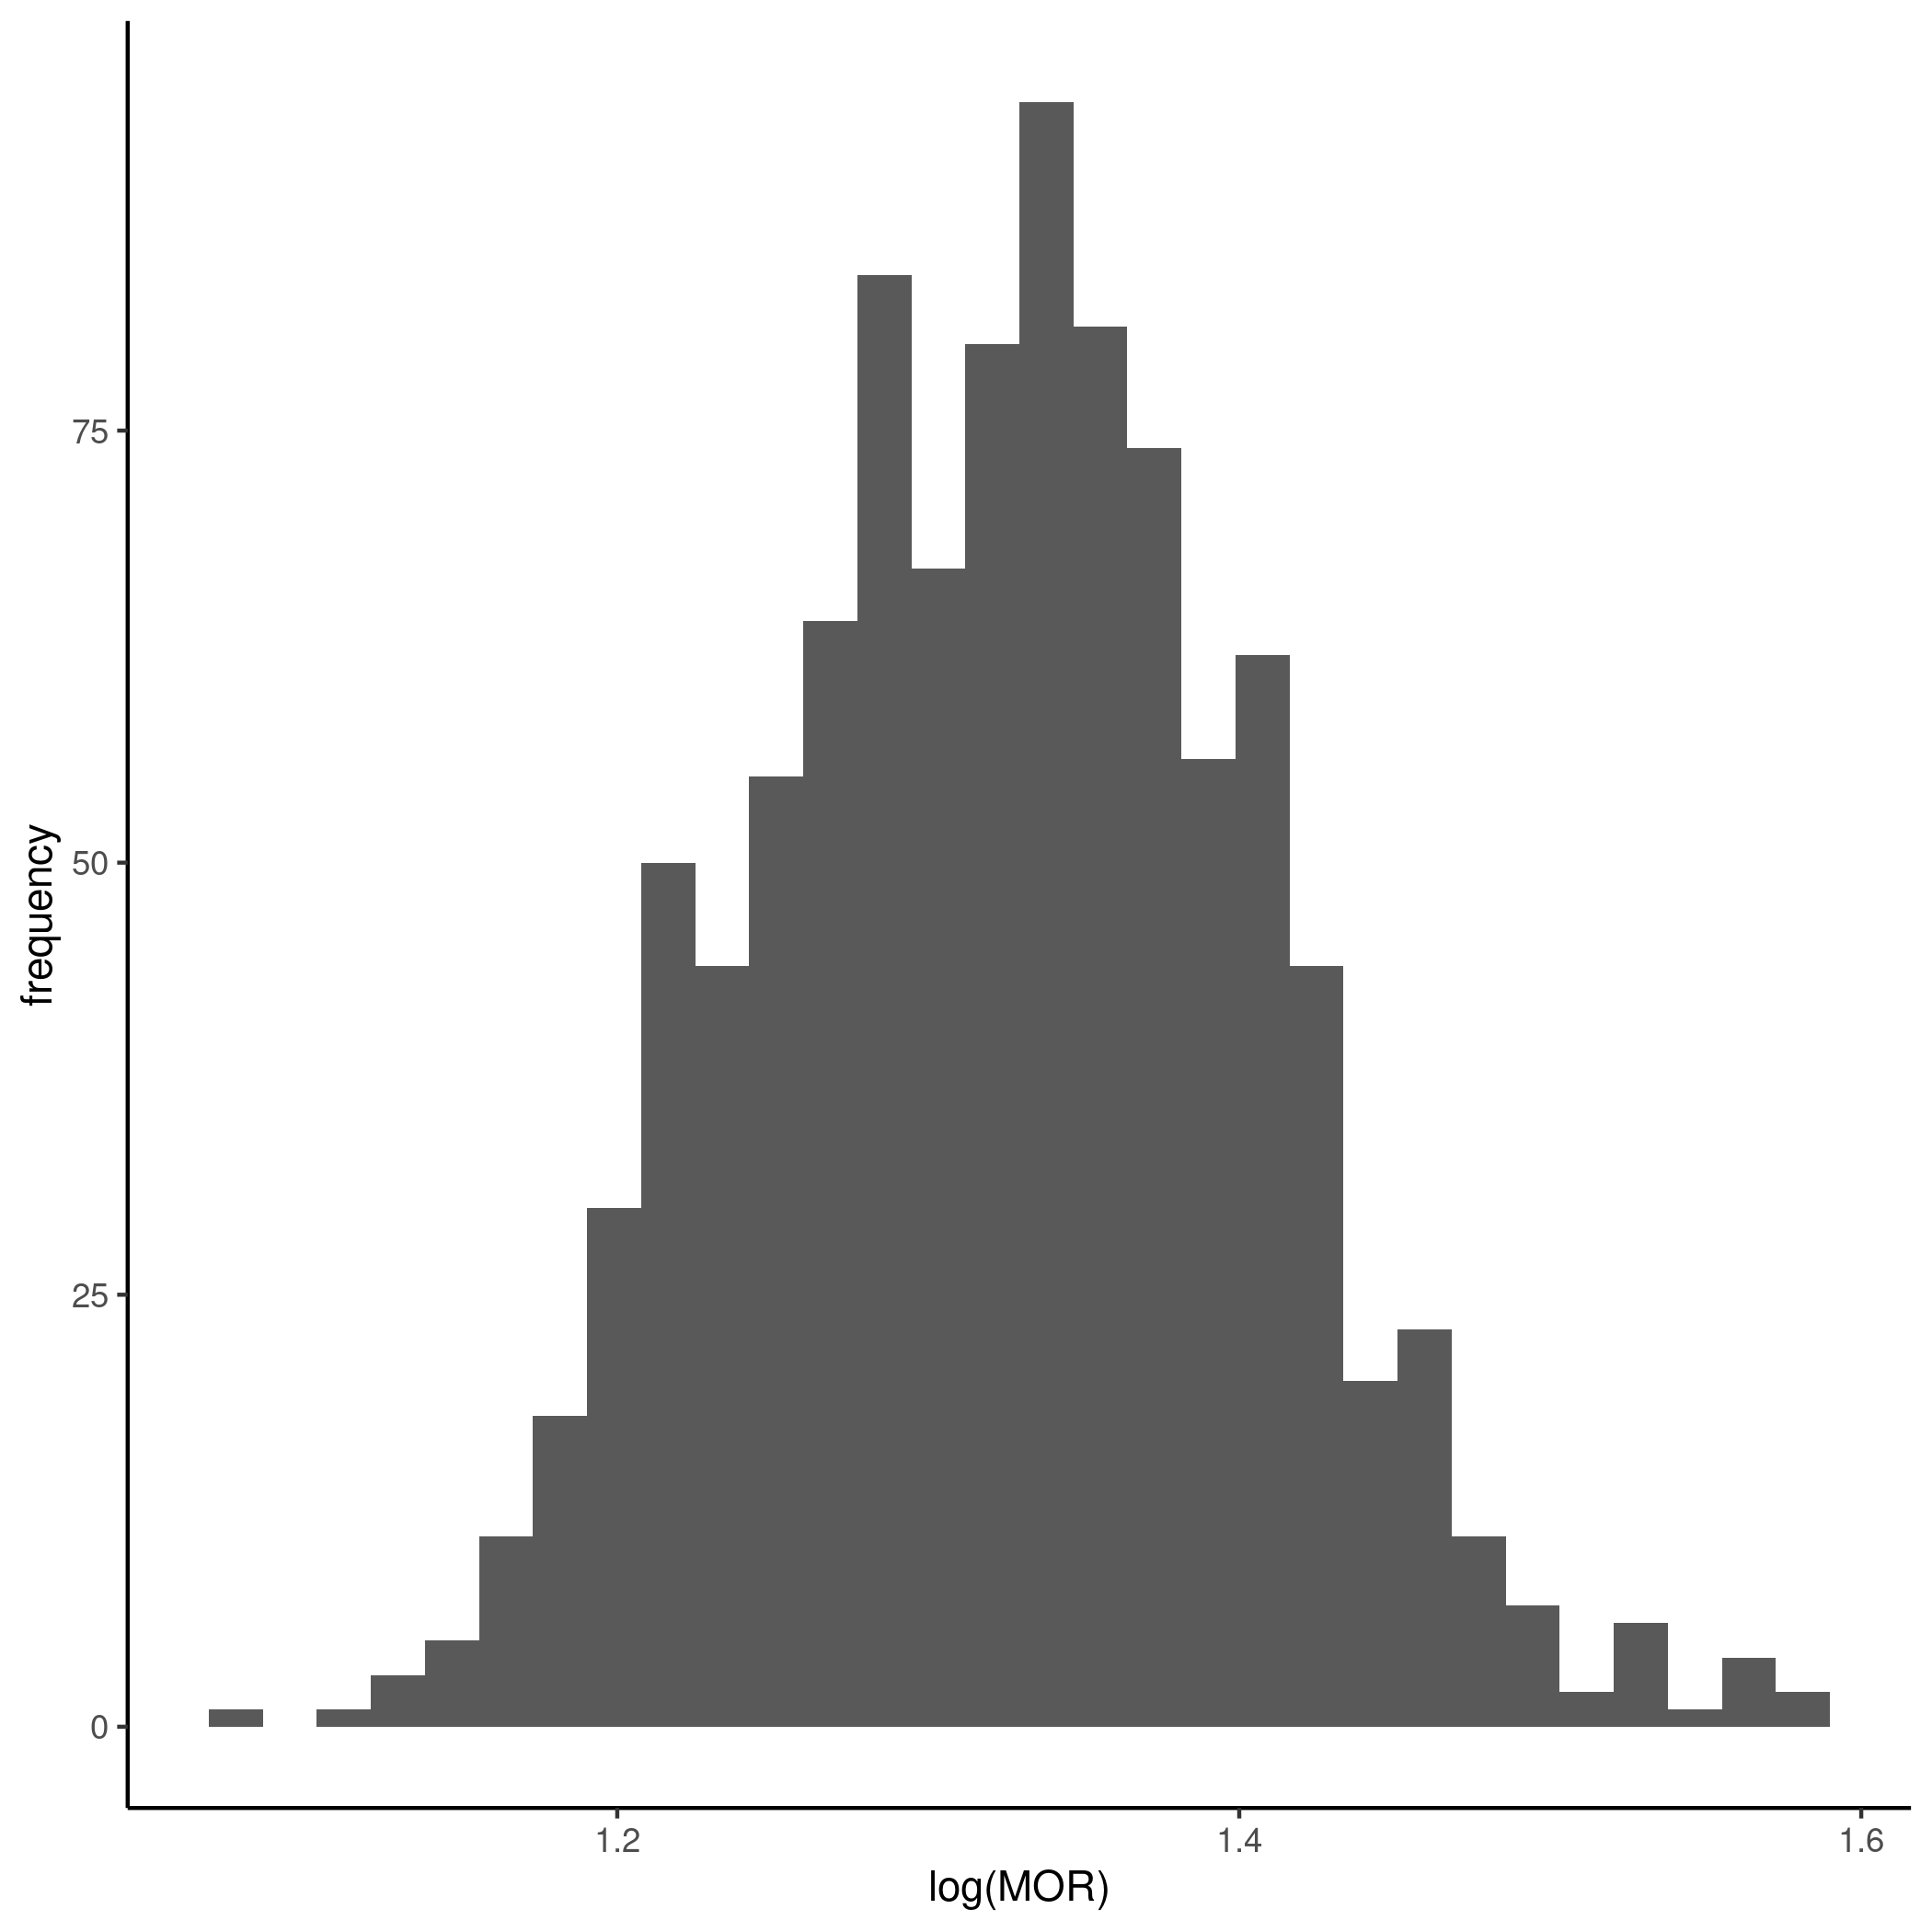
\includegraphics[width=.95\linewidth]{../../plots/three-lvl-ran-int/low-prev/hist_40_10_30_three_lvl_low_prev_mor1.png}  
    \caption{MOR\textsubscript{1}}
    \label{l40m10n301}
\end{subfigure}
\begin{subfigure}{.49\textwidth}
    \centering
    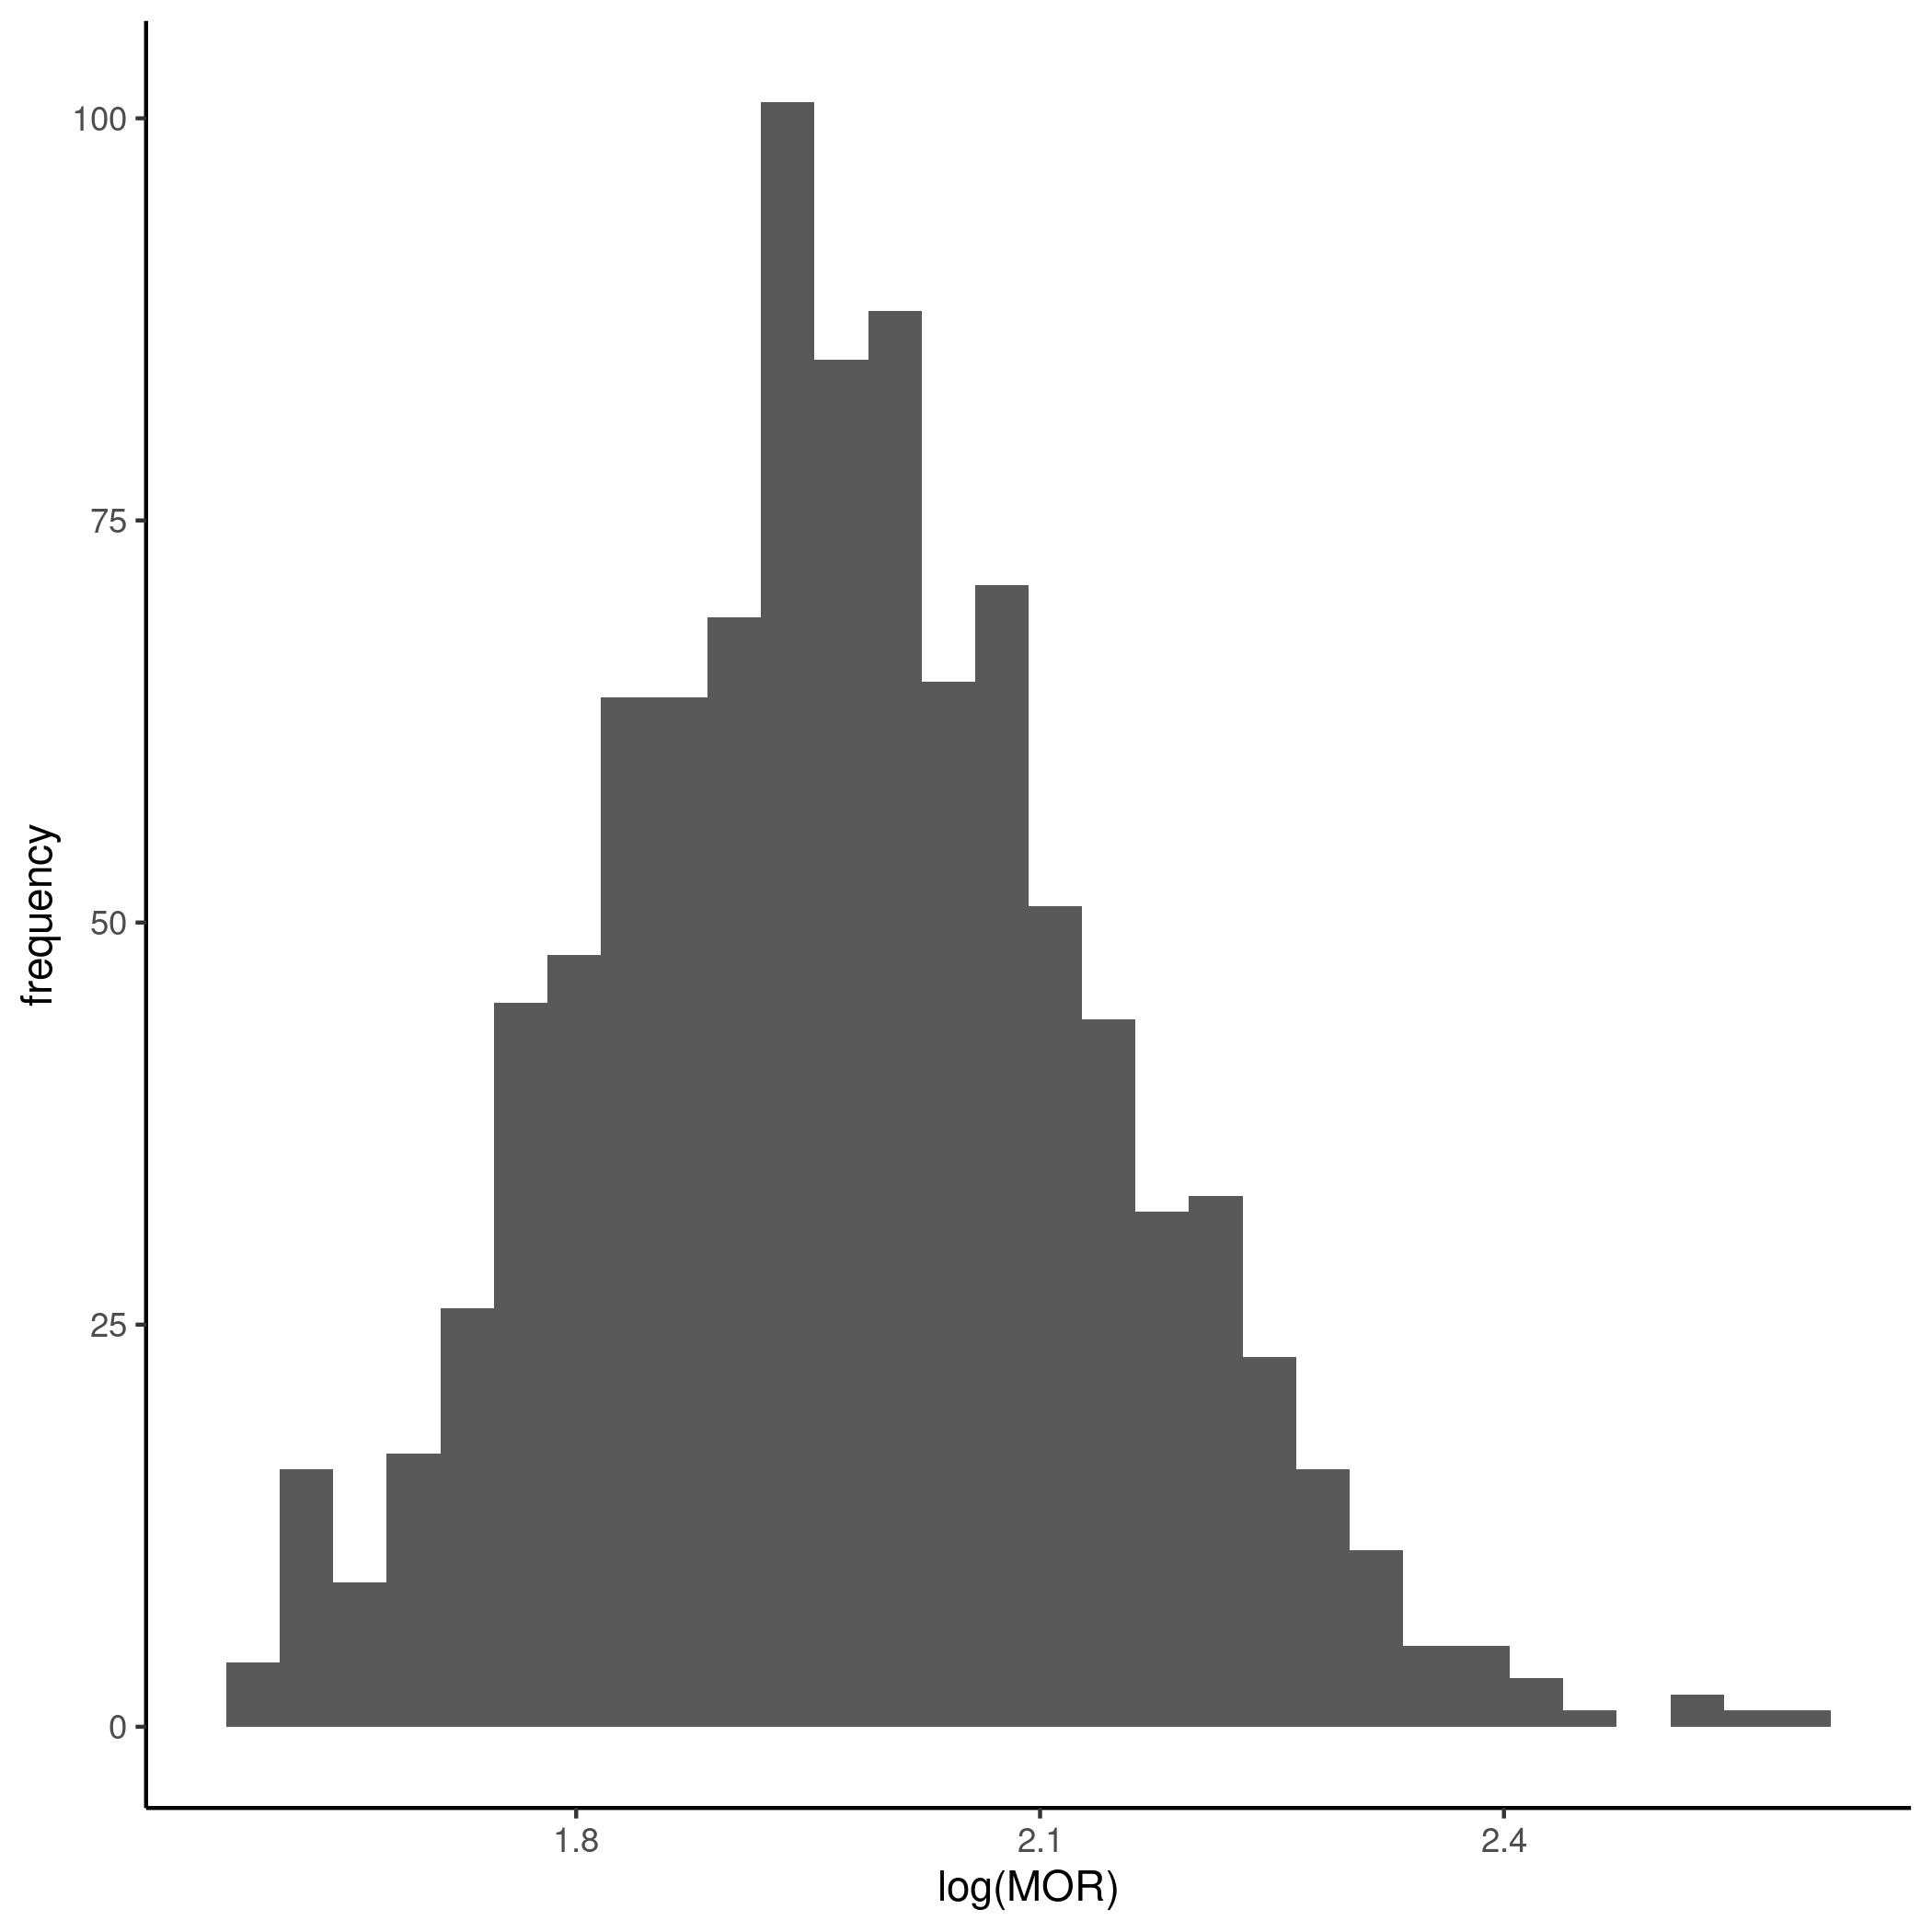
\includegraphics[width=.95\linewidth]{../../plots/three-lvl-ran-int/low-prev/hist_40_10_30_three_lvl_low_prev_mor2.png}
    \caption{MOR\textsubscript{2}}
    \label{l40m10n302}
\end{subfigure}
\caption{Hospitals = 40, Doctors = 10, Patients = 30}
\label{mor2}
\end{figure}

\vspace{10mm}

\begin{figure}
\centering
\begin{subfigure}{.49\textwidth}
    \centering
    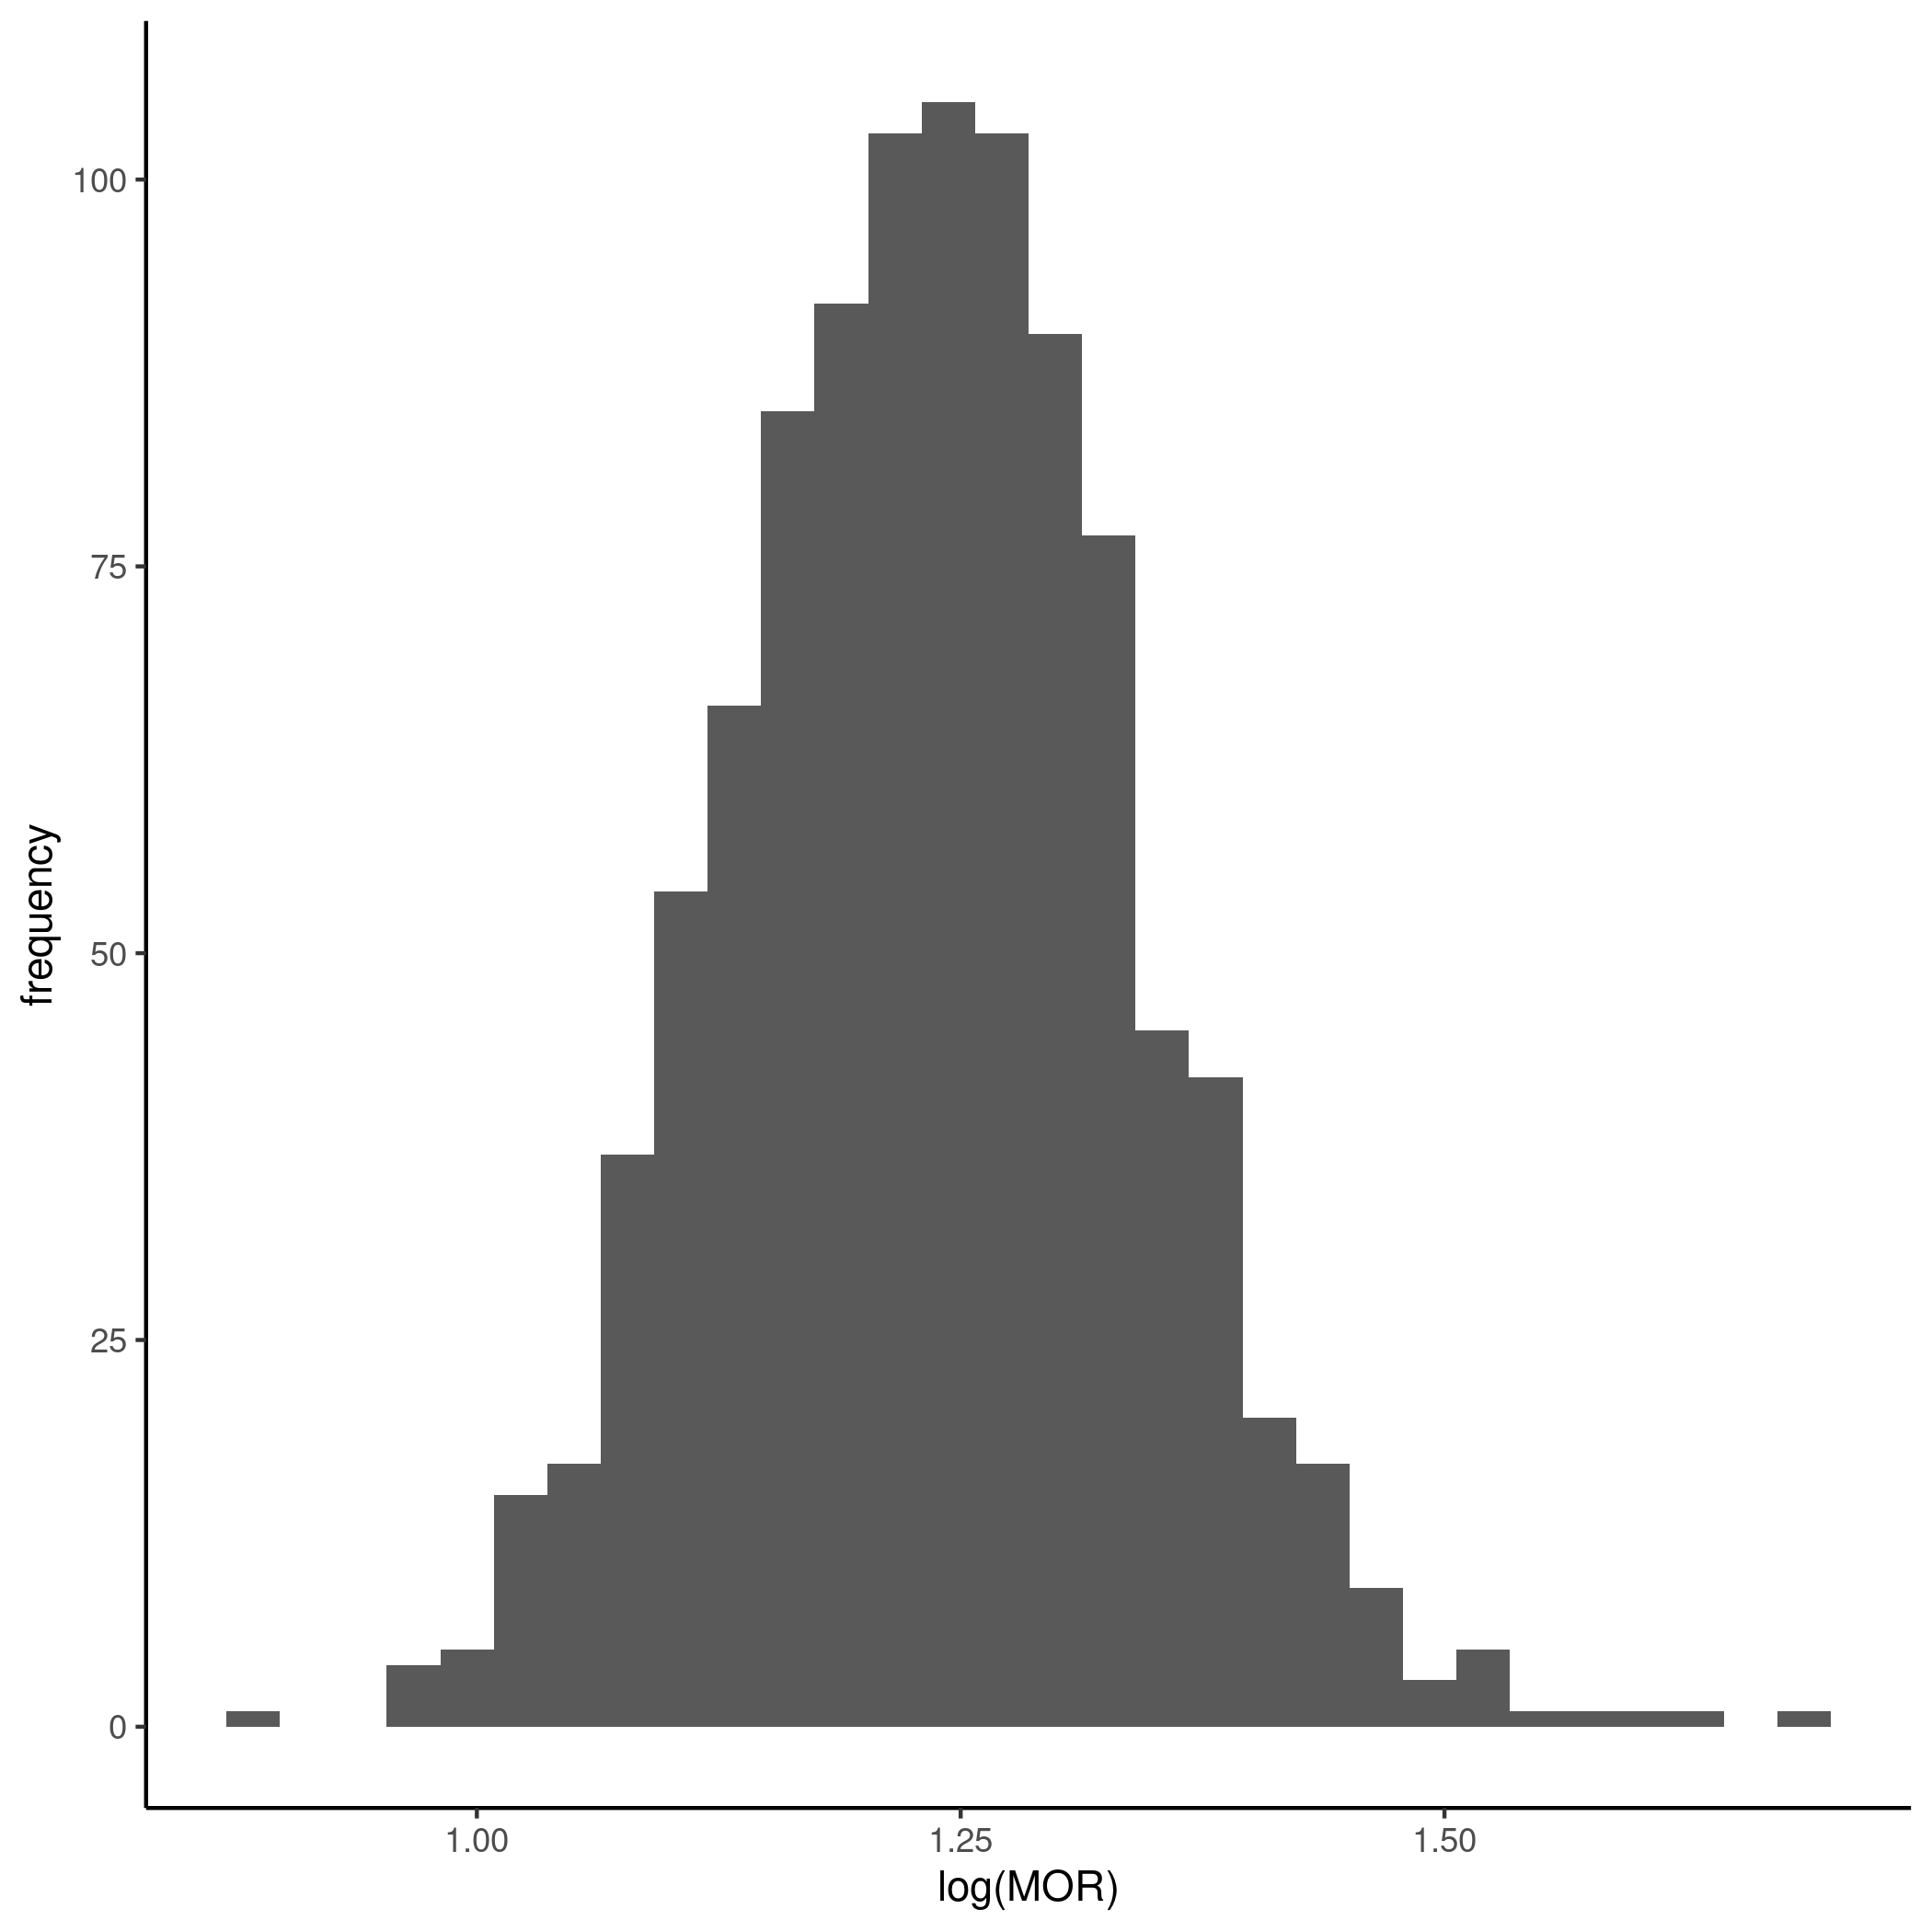
\includegraphics[width=.95\linewidth]{../../plots/three-lvl-ran-int/low-prev/hist_40_30_5_three_lvl_low_prev_mor1.png}  
    \caption{MOR\textsubscript{1}}
    \label{l40m30n51}
\end{subfigure}
\begin{subfigure}{.49\textwidth}
    \centering
    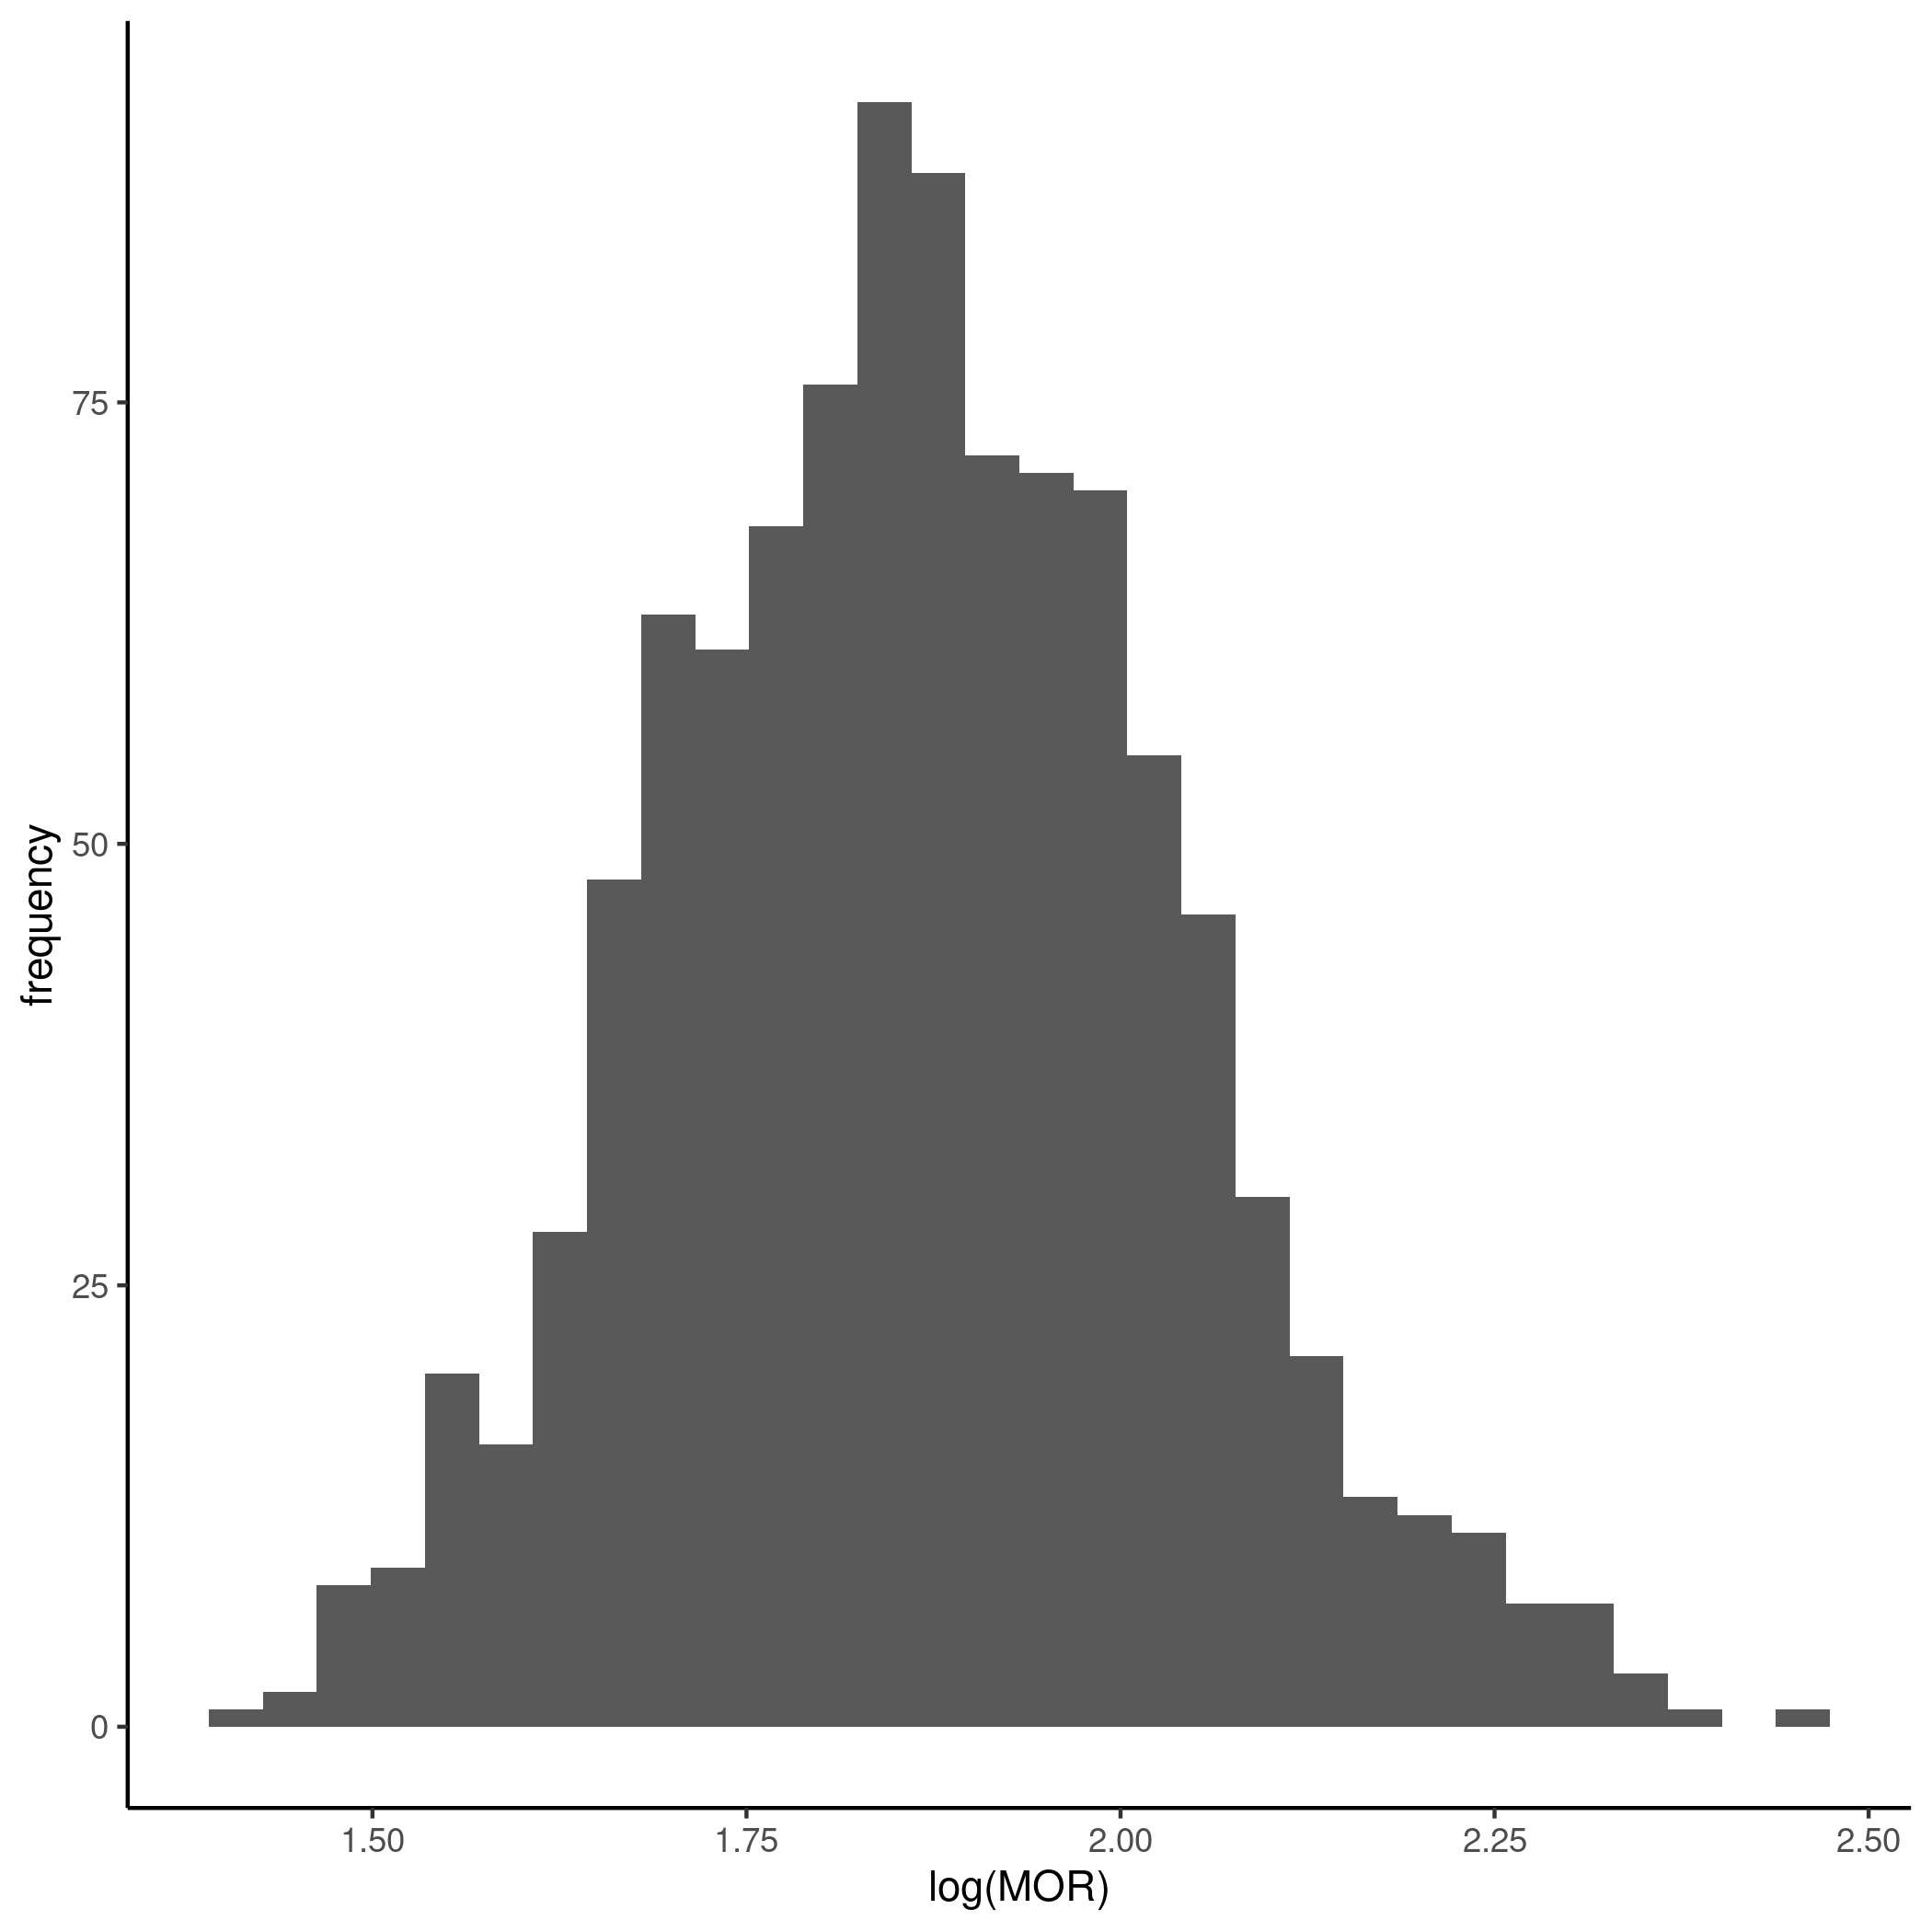
\includegraphics[width=.95\linewidth]{../../plots/three-lvl-ran-int/low-prev/hist_40_30_5_three_lvl_low_prev_mor2.png}
    \caption{MOR\textsubscript{2}}
    \label{l40m30n52}
\end{subfigure}
\caption{Hospitals = 40, Doctors = 30, Patients = 5}
\label{mor2}
\end{figure}

\vspace{10mm}

\begin{figure}
\centering
\begin{subfigure}{.49\textwidth}
    \centering
    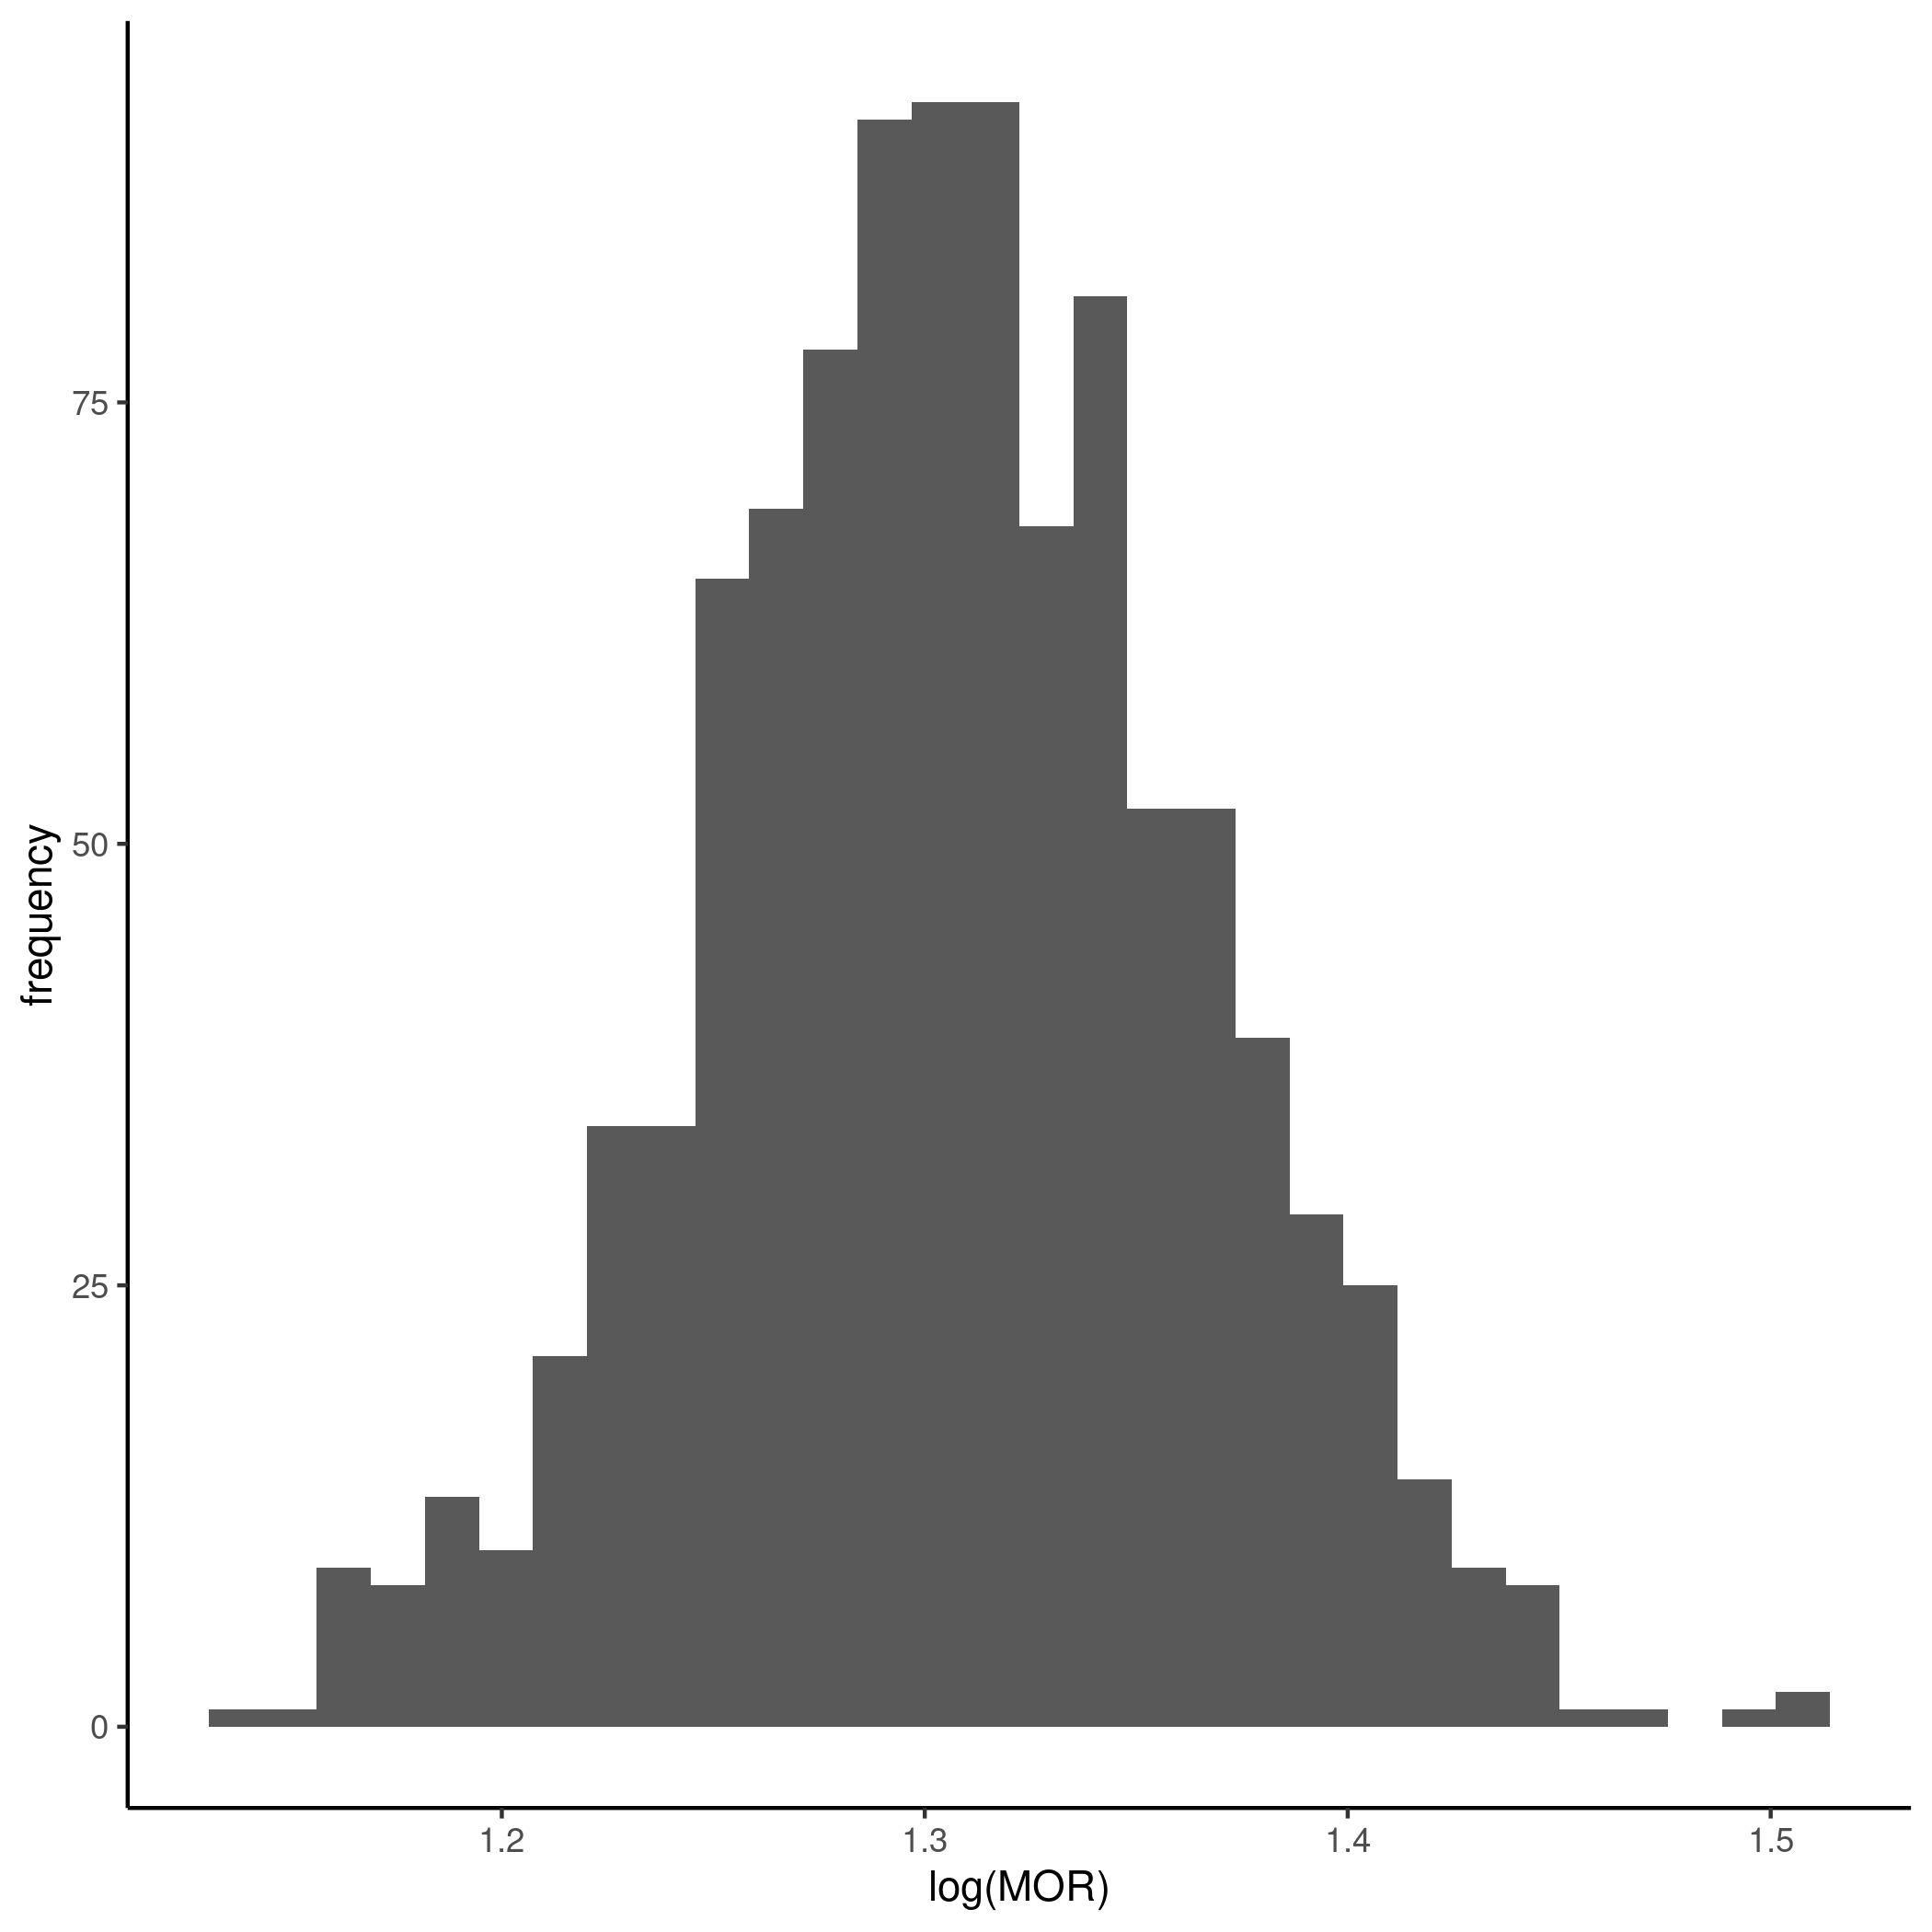
\includegraphics[width=.95\linewidth]{../../plots/three-lvl-ran-int/low-prev/hist_40_30_15_three_lvl_low_prev_mor1.png}  
    \caption{MOR\textsubscript{1}}
    \label{l40m30n151}
\end{subfigure}
\begin{subfigure}{.49\textwidth}
    \centering
    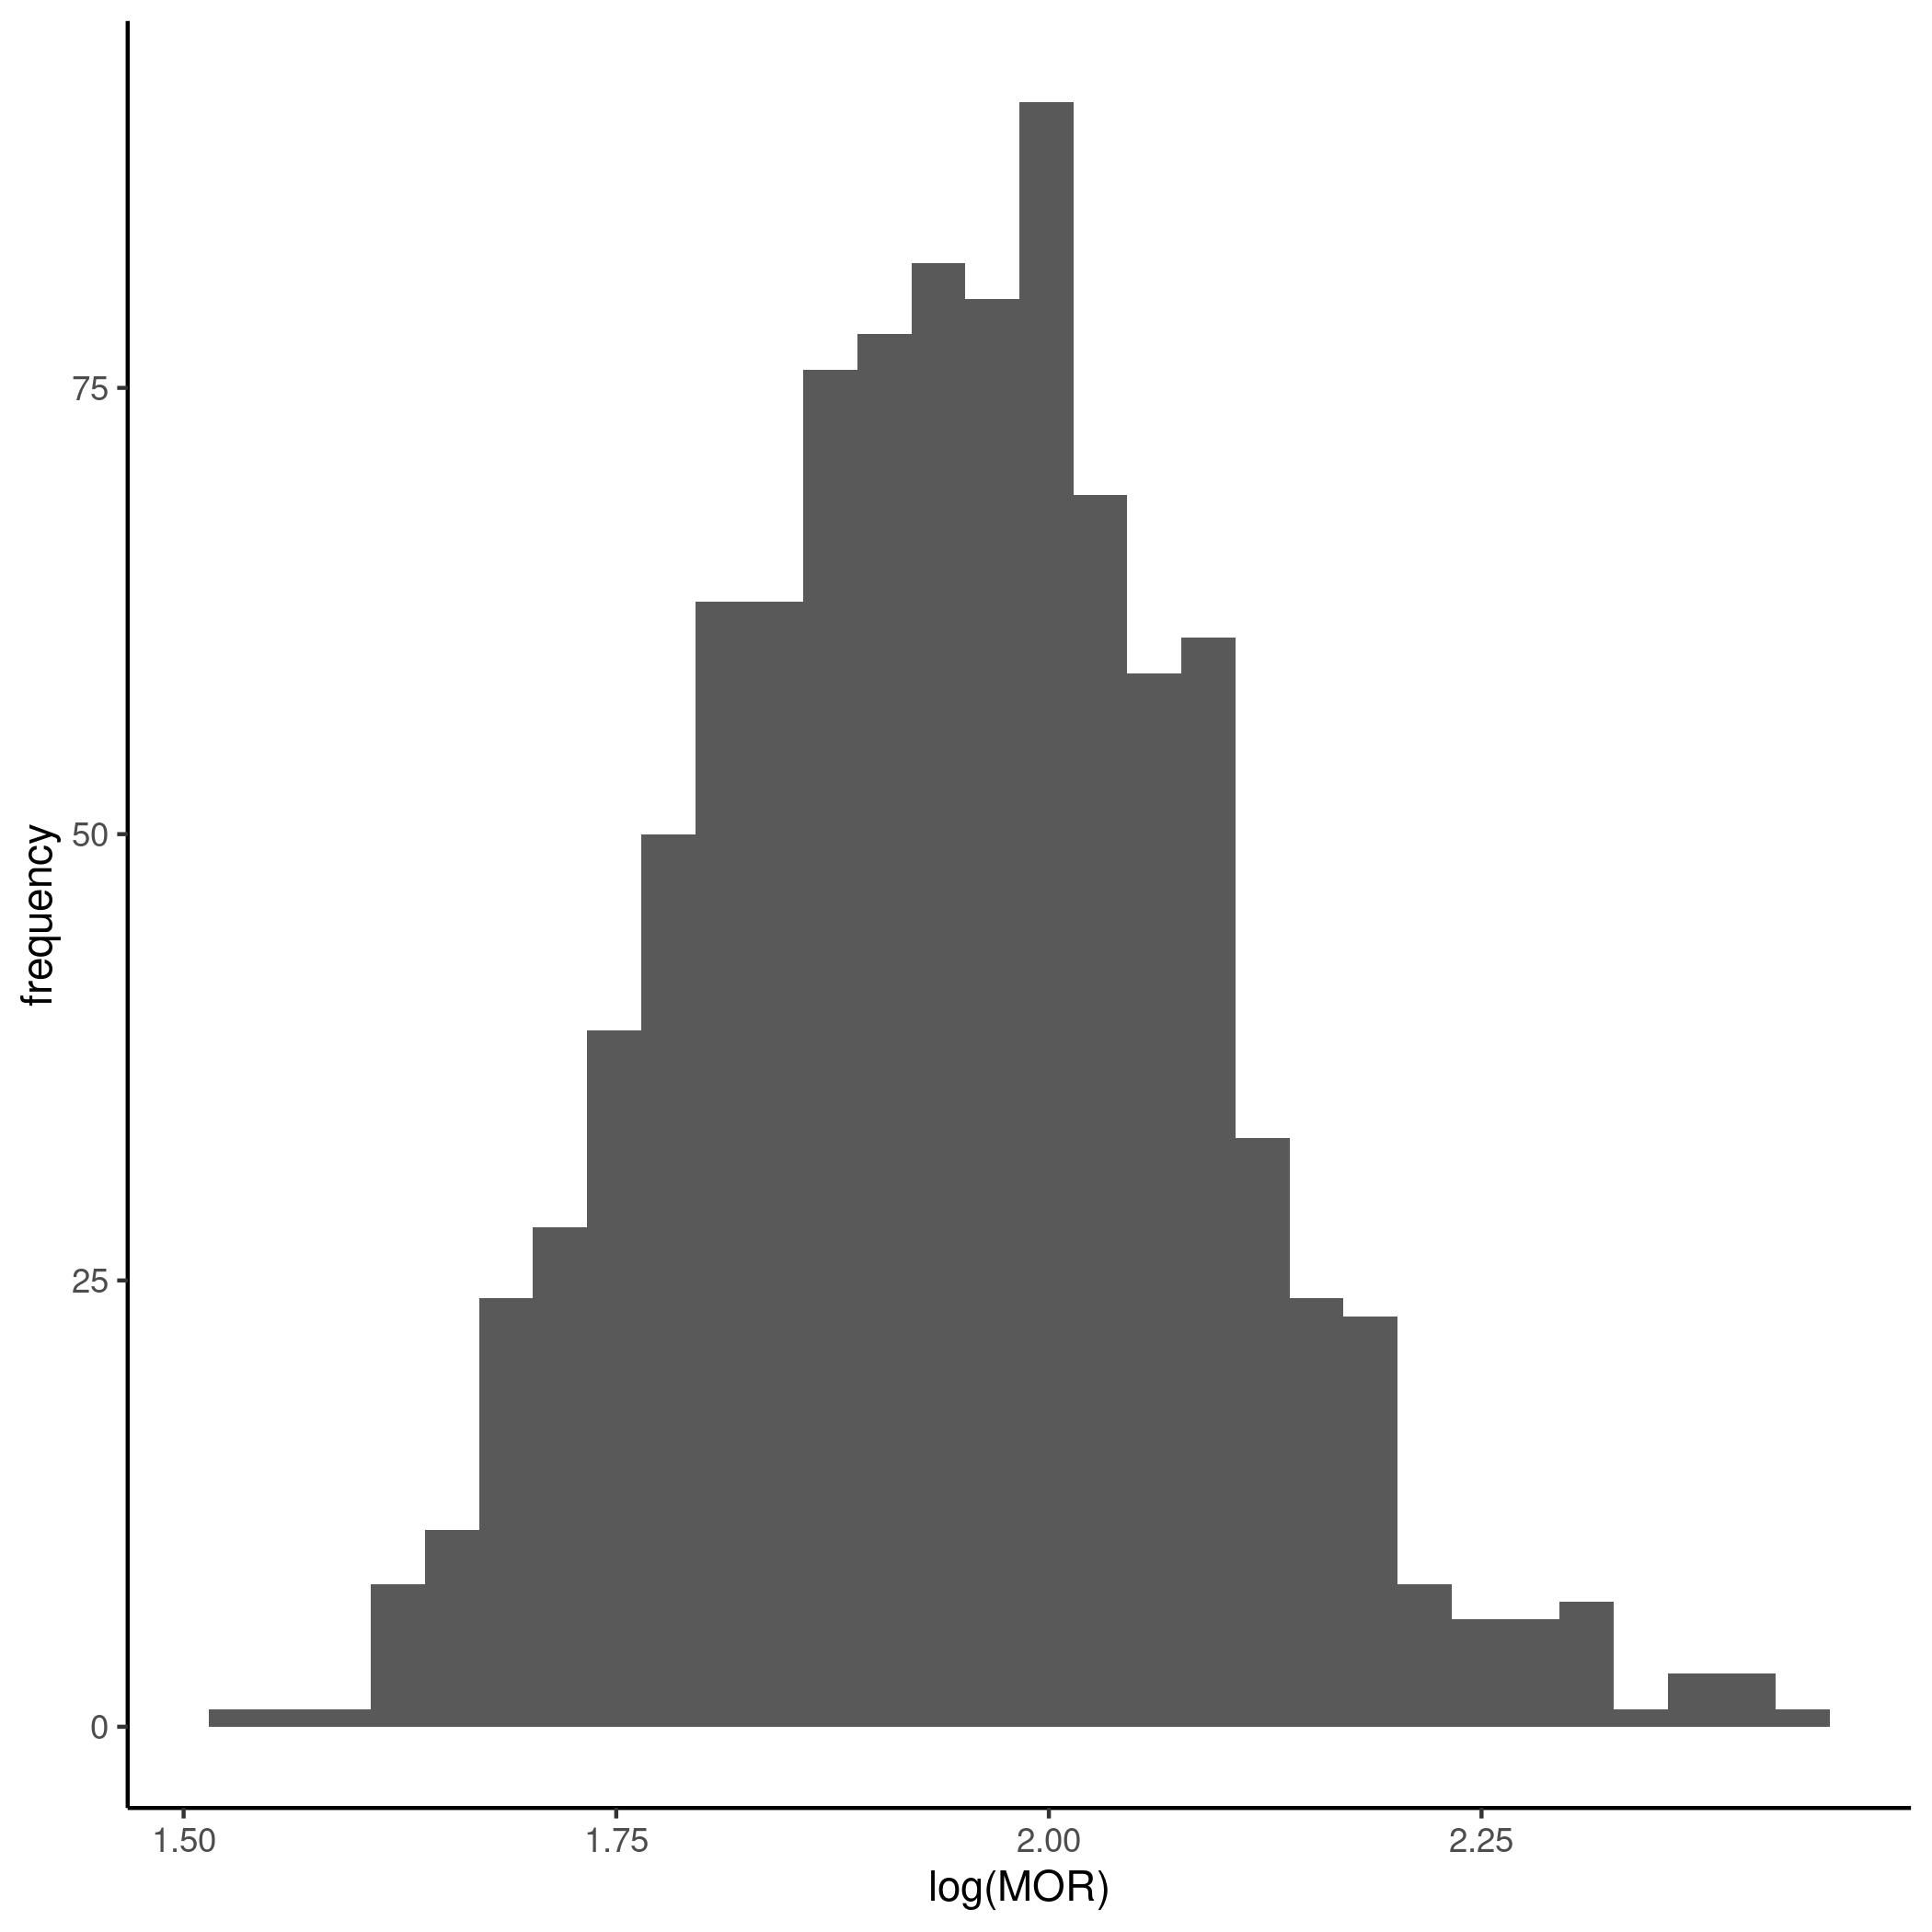
\includegraphics[width=.95\linewidth]{../../plots/three-lvl-ran-int/low-prev/hist_40_30_15_three_lvl_low_prev_mor2.png}
    \caption{MOR\textsubscript{2}}
    \label{l40m30n152}
\end{subfigure}
\caption{Hospitals = 40, Doctors = 30, Patients = 15}
\label{mor2}
\end{figure}

\vspace{10mm}

\begin{figure}
\centering
\begin{subfigure}{.49\textwidth}
    \centering
    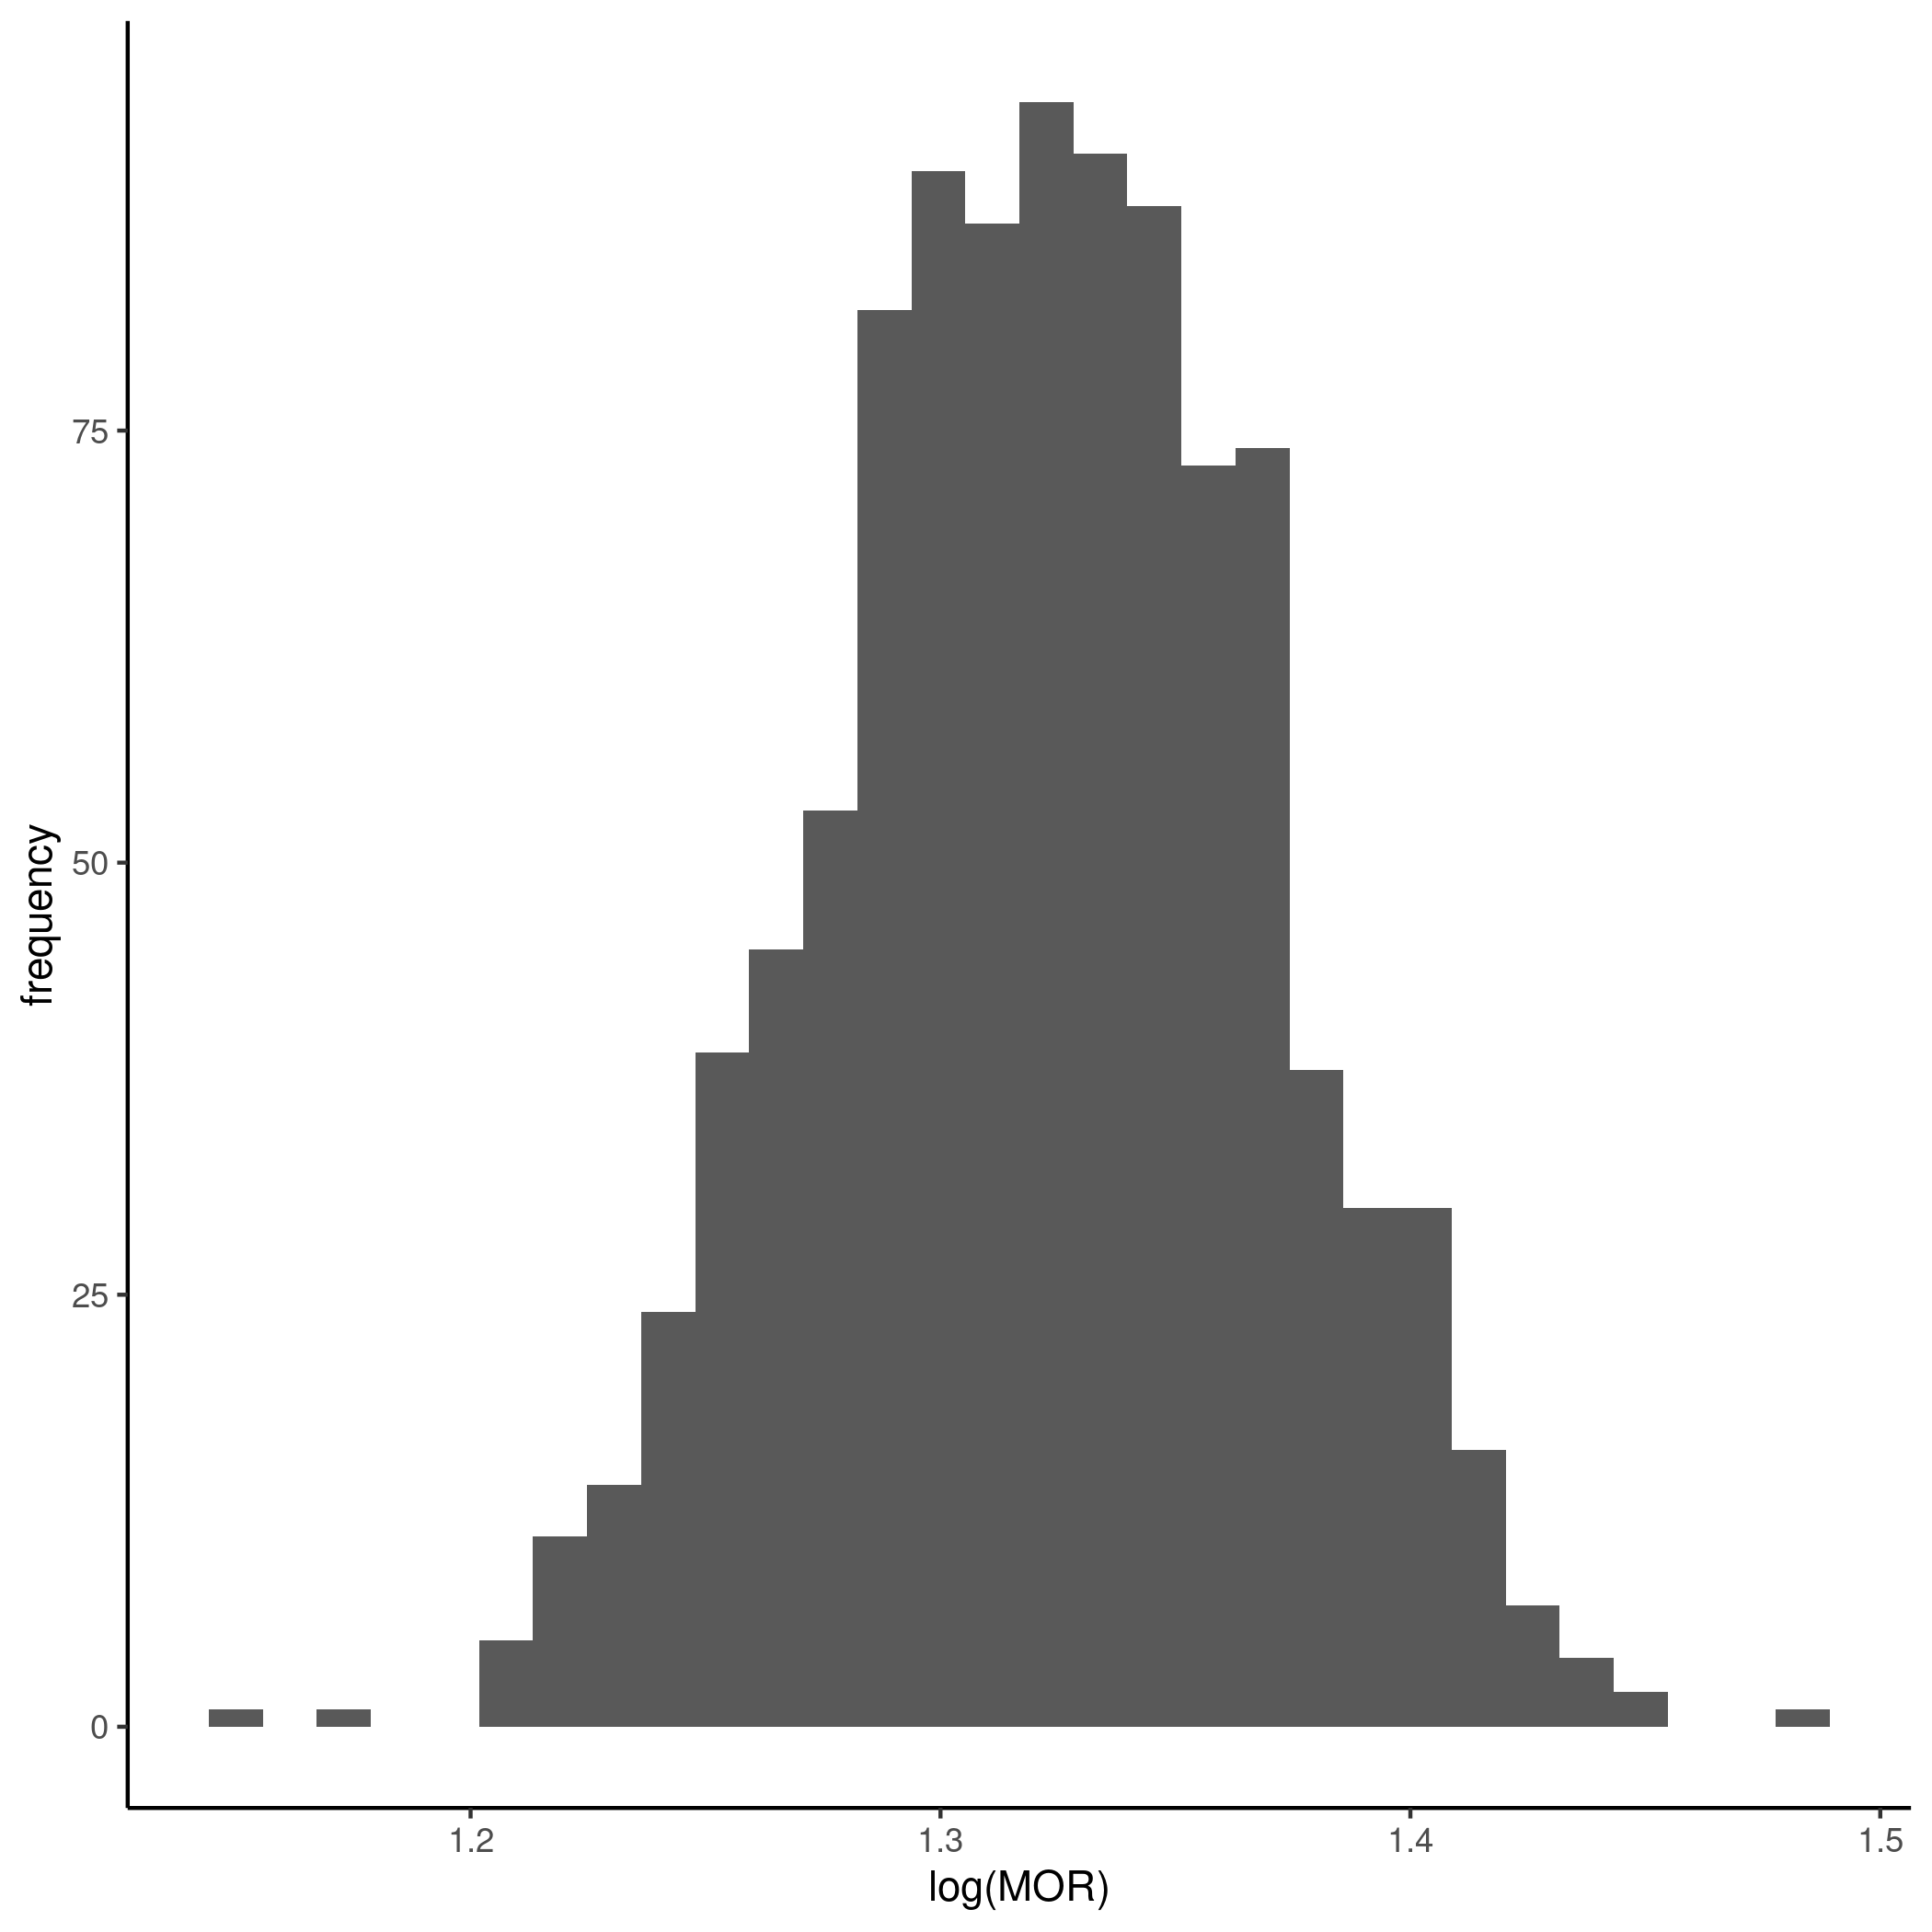
\includegraphics[width=.95\linewidth]{../../plots/three-lvl-ran-int/low-prev/hist_40_30_30_three_lvl_low_prev_mor1.png}  
    \caption{MOR\textsubscript{1}}
    \label{l40m30n301}
\end{subfigure}
\begin{subfigure}{.49\textwidth}
    \centering
    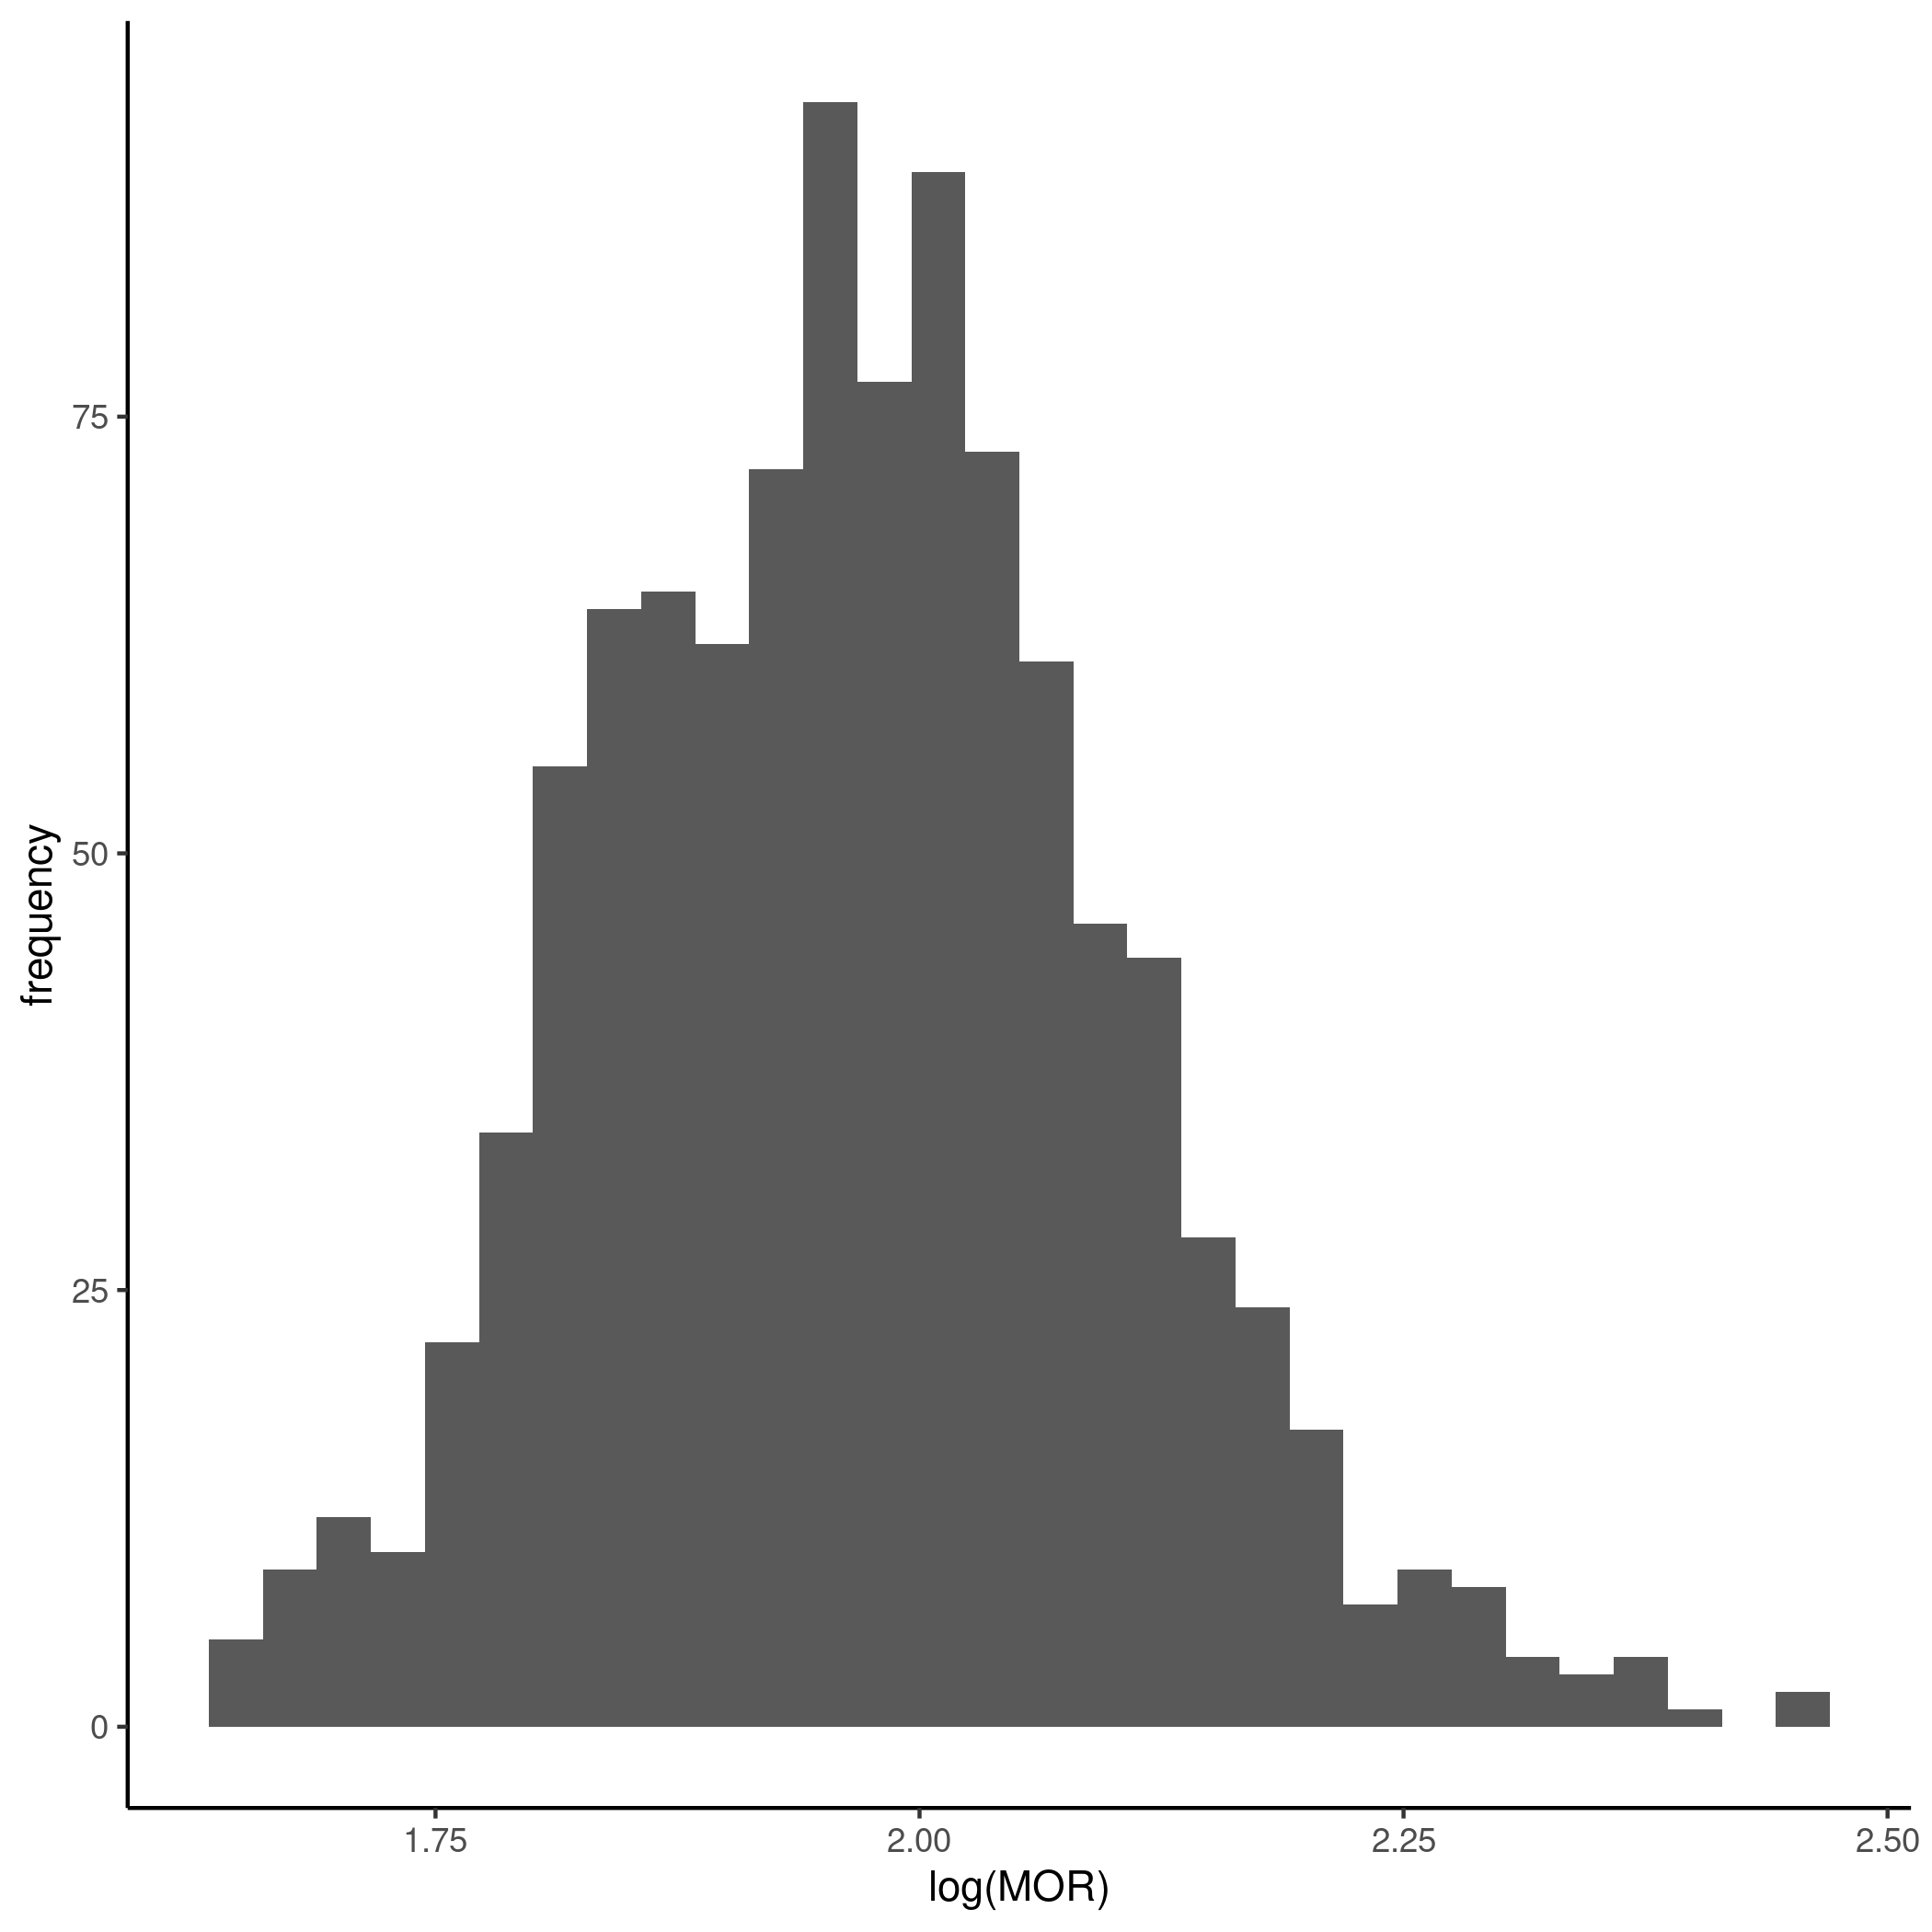
\includegraphics[width=.95\linewidth]{../../plots/three-lvl-ran-int/low-prev/hist_40_30_30_three_lvl_low_prev_mor2.png}
    \caption{MOR\textsubscript{2}}
    \label{l40m30n302}
\end{subfigure}
\caption{Hospitals = 40, Doctors = 30, Patients = 30}
\label{mor2}
\end{figure}

\newpage
\newgeometry{right=10mm,left=15mm,top=20mm}

\hypertarget{simulation-result-table-for-mor-of-second-level}{%
\section{Simulation Result Table for MOR of Second
Level}\label{simulation-result-table-for-mor-of-second-level}}

\begingroup

\fontsize{8pt}{16pt}\selectfont

\begin{tabular}[t]{>{\centering\arraybackslash}m{0.6cm}>{\centering\arraybackslash}m{0.6cm}>{\centering\arraybackslash}m{0.6cm}>{\centering\arraybackslash}m{0.7cm}>{\centering\arraybackslash}m{0.7cm}>{\centering\arraybackslash}m{0.7cm}>{\centering\arraybackslash}m{0.7cm}>{\centering\arraybackslash}m{0.7cm}>{\centering\arraybackslash}m{1cm}>{\centering\arraybackslash}m{1cm}>{\centering\arraybackslash}m{1cm}>{\centering\arraybackslash}m{1cm}>{\centering\arraybackslash}m{1cm}>{\centering\arraybackslash}m{1cm}>{\centering\arraybackslash}m{1cm}}
\toprule
L\textsuperscript{1} & M\textsuperscript{2} & N\textsuperscript{3} & $\widehat{\beta_0}$ & $\widehat{\beta_1}$ & $\widehat{\beta_2}$ & $\widehat{\sigma^2_{u_{jk}}}$ & $\widehat{\sigma^2_{v_k}}$ & $\widehat{MOR_1}$ & Rel. Bias (\%) & $\widehat{SE}_{MOR}$ & Sim. $\widehat{SE}_{MOR}$ & Ratio\textsuperscript{4} & Coverage\textsuperscript{5} (95\%) & Model Conv\textsuperscript{6}\\
\midrule
20 & 10 & 5 & -4.12 & 1.75 & 0.69 & 1.96 & 2.18 & 3.85 & -0.18 & 1.34 & 1.35 & 0.99 & 0.94 & 0.98\\
20 & 10 & 15 & -4.09 & 1.74 & 0.67 & 1.87 & 2.24 & 3.70 & -3.99 & 1.15 & 1.16 & 0.99 & 0.91 & 1.00\\
20 & 10 & 30 & -4.08 & 1.75 & 0.67 & 1.94 & 2.32 & 3.79 & -1.77 & 1.12 & 1.12 & 1.00 & 0.93 & 1.00\\
\midrule
20 & 30 & 5 & -4.04 & 1.72 & 0.66 & 1.72 & 2.18 & 3.51 & -9.04 & 1.16 & 1.16 & 1.00 & 0.86 & 1.00\\
20 & 30 & 15 & -4.08 & 1.74 & 0.67 & 1.87 & 2.27 & 3.68 & -4.38 & 1.08 & 1.08 & 1.00 & 0.88 & 1.00\\
20 & 30 & 30 & -4.09 & 1.75 & 0.67 & 1.93 & 2.32 & 3.76 & -2.33 & 1.07 & 1.07 & 1.00 & 0.92 & 1.00\\
\midrule
40 & 10 & 5 & -4.08 & 1.73 & 0.66 & 1.83 & 2.21 & 3.66 & -5.01 & 1.21 & 1.23 & 0.99 & 0.90 & 1.00\\
40 & 10 & 15 & -4.07 & 1.75 & 0.67 & 1.89 & 2.35 & 3.72 & -3.58 & 1.11 & 1.11 & 1.00 & 0.92 & 1.00\\
40 & 10 & 30 & -4.09 & 1.75 & 0.67 & 1.94 & 2.39 & 3.77 & -2.08 & 1.08 & 1.08 & 1.00 & 0.93 & 1.00\\
\midrule
40 & 30 & 5 & -4.02 & 1.72 & 0.66 & 1.69 & 2.18 & 3.46 & -10.17 & 1.11 & 1.11 & 1.00 & 0.78 & 1.00\\
40 & 30 & 15 & -4.09 & 1.75 & 0.67 & 1.88 & 2.29 & 3.70 & -3.93 & 1.06 & 1.06 & 1.00 & 0.88 & 1.00\\
40 & 30 & 30 & -4.08 & 1.75 & 0.67 & 1.92 & 2.36 & 3.76 & -2.51 & 1.05 & 1.05 & 1.00 & 0.89 & 1.00\\
\bottomrule
\multicolumn{15}{l}{\rule{0pt}{1em}\textit{Note: }}\\
\multicolumn{15}{l}{\rule{0pt}{1em} }\\
\multicolumn{15}{l}{\rule{0pt}{1em}\textsuperscript{1} Number of Hospital}\\
\multicolumn{15}{l}{\rule{0pt}{1em}\textsuperscript{2} Number of Doctors}\\
\multicolumn{15}{l}{\rule{0pt}{1em}\textsuperscript{3} Number of patients}\\
\multicolumn{15}{l}{\rule{0pt}{1em}\textsuperscript{4} Ratio$\;=\;\dfrac{\widehat{SE}_{MOR}}{Simulation\;\widehat{SE}_{MOR}}$}\\
\multicolumn{15}{l}{\rule{0pt}{1em}\textsuperscript{5} Confidence Interval Coverage Probability}\\
\multicolumn{15}{l}{\rule{0pt}{1em}\textsuperscript{6} Model Convergence (Ratio of 1000 runs to the runs required to get 1000 converged cases)}\\
\multicolumn{15}{l}{\rule{0pt}{1em}\textsuperscript{*} The mean prevalence for this simulation is 12\%}\\
\multicolumn{15}{l}{\rule{0pt}{1em}\textsuperscript{\dag} True $MOR_1$ is 3.85}\\
\multicolumn{15}{l}{\rule{0pt}{1em}\textsuperscript{\ddag} True $\sigma^2_{u_{jk}}$ is 2}\\
\multicolumn{15}{l}{\rule{0pt}{1em}\textsuperscript{\S} True $\sigma^2_{v_k}$ is 2.5}\\
\multicolumn{15}{l}{\rule{0pt}{1em}\textsuperscript{\P} True Values of $\beta_0 = -4.1$, $\beta_1 = 1.75$, $\beta_2 = 0.67$}\\
\end{tabular}

\endgroup

\hypertarget{simulation-result-table-for-mor-of-third-level}{%
\section{Simulation Result Table for MOR of Third
Level}\label{simulation-result-table-for-mor-of-third-level}}

\begingroup

\fontsize{8pt}{16pt}\selectfont

\begin{tabular}[t]{>{\centering\arraybackslash}m{0.6cm}>{\centering\arraybackslash}m{0.6cm}>{\centering\arraybackslash}m{0.6cm}>{\centering\arraybackslash}m{0.7cm}>{\centering\arraybackslash}m{0.7cm}>{\centering\arraybackslash}m{0.7cm}>{\centering\arraybackslash}m{0.7cm}>{\centering\arraybackslash}m{0.7cm}>{\centering\arraybackslash}m{1cm}>{\centering\arraybackslash}m{1cm}>{\centering\arraybackslash}m{1cm}>{\centering\arraybackslash}m{1cm}>{\centering\arraybackslash}m{1cm}>{\centering\arraybackslash}m{1cm}>{\centering\arraybackslash}m{1cm}}
\toprule
L\textsuperscript{1} & M\textsuperscript{2} & N\textsuperscript{3} & $\widehat{\beta_0}$ & $\widehat{\beta_1}$ & $\widehat{\beta_2}$ & $\widehat{\sigma^2_{u_{jk}}}$ & $\widehat{\sigma^2_{v_k}}$ & $\widehat{MOR_2}$ & Rel. Bias (\%) & $\widehat{SE}_{MOR}$ & Sim. $\widehat{SE}_{MOR}$ & Ratio\textsuperscript{4} & Coverage\textsuperscript{5} (95\%) & Model Conv\textsuperscript{6}\\
\midrule
20 & 10 & 5 & -4.12 & 1.75 & 0.69 & 1.96 & 2.18 & 7.19 & -5.00 & 1.39 & 1.42 & 0.98 & 0.89 & 0.98\\
20 & 10 & 15 & -4.09 & 1.74 & 0.67 & 1.87 & 2.24 & 7.04 & -6.97 & 1.26 & 1.28 & 0.98 & 0.86 & 1.00\\
20 & 10 & 30 & -4.08 & 1.75 & 0.67 & 1.94 & 2.32 & 7.26 & -3.97 & 1.24 & 1.25 & 0.99 & 0.89 & 1.00\\
\midrule
20 & 30 & 5 & -4.04 & 1.72 & 0.66 & 1.72 & 2.18 & 6.68 & -11.66 & 1.25 & 1.28 & 0.98 & 0.80 & 1.00\\
20 & 30 & 15 & -4.08 & 1.74 & 0.67 & 1.87 & 2.27 & 7.04 & -6.95 & 1.21 & 1.22 & 0.99 & 0.85 & 1.00\\
20 & 30 & 30 & -4.09 & 1.75 & 0.67 & 1.93 & 2.32 & 7.21 & -4.65 & 1.20 & 1.21 & 1.00 & 0.87 & 1.00\\
\midrule
40 & 10 & 5 & -4.08 & 1.73 & 0.66 & 1.83 & 2.21 & 6.91 & -8.66 & 1.25 & 1.26 & 0.99 & 0.87 & 1.00\\
40 & 10 & 15 & -4.07 & 1.75 & 0.67 & 1.89 & 2.35 & 7.19 & -4.95 & 1.18 & 1.21 & 0.98 & 0.86 & 1.00\\
40 & 10 & 30 & -4.09 & 1.75 & 0.67 & 1.94 & 2.39 & 7.32 & -3.26 & 1.17 & 1.18 & 0.99 & 0.89 & 1.00\\
\midrule
40 & 30 & 5 & -4.02 & 1.72 & 0.66 & 1.69 & 2.18 & 6.57 & -13.10 & 1.17 & 1.19 & 0.99 & 0.75 & 1.00\\
40 & 30 & 15 & -4.09 & 1.75 & 0.67 & 1.88 & 2.29 & 7.05 & -6.75 & 1.15 & 1.16 & 0.99 & 0.84 & 1.00\\
40 & 30 & 30 & -4.08 & 1.75 & 0.67 & 1.92 & 2.36 & 7.24 & -4.27 & 1.14 & 1.14 & 1.00 & 0.89 & 1.00\\
\bottomrule
\multicolumn{15}{l}{\rule{0pt}{1em}\textit{Note: }}\\
\multicolumn{15}{l}{\rule{0pt}{1em} }\\
\multicolumn{15}{l}{\rule{0pt}{1em}\textsuperscript{1} Number of Hospital}\\
\multicolumn{15}{l}{\rule{0pt}{1em}\textsuperscript{2} Number of Doctors}\\
\multicolumn{15}{l}{\rule{0pt}{1em}\textsuperscript{3} Number of patients}\\
\multicolumn{15}{l}{\rule{0pt}{1em}\textsuperscript{4} Ratio$\;=\;\dfrac{\widehat{SE}_{MOR}}{Simulation\;\widehat{SE}_{MOR}}$}\\
\multicolumn{15}{l}{\rule{0pt}{1em}\textsuperscript{5} Confidence Interval Coverage Probability}\\
\multicolumn{15}{l}{\rule{0pt}{1em}\textsuperscript{6} Model Convergence (Ratio of 1000 runs to the runs required to get 1000 converged cases)}\\
\multicolumn{15}{l}{\rule{0pt}{1em}\textsuperscript{*} The mean prevalence for this simulation is 12\%}\\
\multicolumn{15}{l}{\rule{0pt}{1em}\textsuperscript{\dag} True $MOR_2$ is 7.56}\\
\multicolumn{15}{l}{\rule{0pt}{1em}\textsuperscript{\ddag} True $\sigma^2_{u_{jk}}$ is 2}\\
\multicolumn{15}{l}{\rule{0pt}{1em}\textsuperscript{\S} True $\sigma^2_{v_k}$ is 2.5}\\
\multicolumn{15}{l}{\rule{0pt}{1em}\textsuperscript{\P} True Values of $\beta_0 = -4.1$, $\beta_1 = 1.75$, $\beta_2 = 0.67$}\\
\end{tabular}

\endgroup

\newpage

\KOMAoptions{usegeometry,paper=landscape,pagesize}
\recalctypearea
\newgeometry{right=10mm,left=10mm,top=15mm,bottom=2mm}

\hypertarget{simulation-result-table-all-together}{%
\section{Simulation Result Table All
Together}\label{simulation-result-table-all-together}}

\begingroup

\fontsize{8pt}{14pt}\selectfont

\begin{tabular}[t]{>{\centering\arraybackslash}m{0.4cm}>{\centering\arraybackslash}m{0.4cm}>{\centering\arraybackslash}m{0.4cm}>{\centering\arraybackslash}m{0.7cm}>{\centering\arraybackslash}m{0.7cm}>{\centering\arraybackslash}m{0.7cm}>{\centering\arraybackslash}m{0.7cm}>{\centering\arraybackslash}m{0.7cm}>{\centering\arraybackslash}m{0.95cm}>{\centering\arraybackslash}m{0.95cm}>{\centering\arraybackslash}m{0.95cm}>{\centering\arraybackslash}m{0.95cm}>{\centering\arraybackslash}m{0.95cm}>{\centering\arraybackslash}m{0.95cm}>{\centering\arraybackslash}m{0.95cm}>{\centering\arraybackslash}m{0.95cm}>{\centering\arraybackslash}m{0.95cm}>{\centering\arraybackslash}m{0.95cm}>{\centering\arraybackslash}m{0.95cm}>{\centering\arraybackslash}m{0.95cm}>{\centering\arraybackslash}m{0.95cm}}
\toprule
\multicolumn{8}{c}{ } & \multicolumn{6}{c}{$MOR_1$} & \multicolumn{6}{c}{$MOR_2$} & \multicolumn{1}{c}{ } \\
\cmidrule(l{3pt}r{3pt}){9-14} \cmidrule(l{3pt}r{3pt}){15-20}
L\textsuperscript{1} & M\textsuperscript{2} & N\textsuperscript{3} & $\widehat{\beta_0}$ & $\widehat{\beta_1}$ & $\widehat{\beta_2}$ & $\widehat{\sigma^2_{u_{jk}}}$ & $\widehat{\sigma^2_{v_k}}$ & $\widehat{MOR}$ & Rel. Bias (\%) & $\widehat{SE}_{MOR}$ & Sim. $\widehat{SE}_{MOR}$ & Ratio\textsuperscript{4} & Coverage\textsuperscript{5} (95\%) & $\widehat{MOR}$ & Rel. Bias (\%) & $\widehat{SE}_{MOR}$ & Sim. $\widehat{SE}_{MOR}$ & Ratio\textsuperscript{4} & Coverage\textsuperscript{5} (95\%) & Model Conv\textsuperscript{6}\\
\midrule
20 & 10 & 5 & -4.12 & 1.75 & 0.69 & 1.96 & 2.18 & 3.85 & -0.18 & 1.34 & 1.35 & 0.99 & 0.94 & 7.19 & -5.00 & 1.39 & 1.42 & 0.98 & 0.89 & 0.98\\
20 & 10 & 15 & -4.09 & 1.74 & 0.67 & 1.87 & 2.24 & 3.70 & -3.99 & 1.15 & 1.16 & 0.99 & 0.91 & 7.04 & -6.97 & 1.26 & 1.28 & 0.98 & 0.86 & 1.00\\
20 & 10 & 30 & -4.08 & 1.75 & 0.67 & 1.94 & 2.32 & 3.79 & -1.77 & 1.12 & 1.12 & 1.00 & 0.93 & 7.26 & -3.97 & 1.24 & 1.25 & 0.99 & 0.89 & 1.00\\
\midrule
20 & 30 & 5 & -4.04 & 1.72 & 0.66 & 1.72 & 2.18 & 3.51 & -9.04 & 1.16 & 1.16 & 1.00 & 0.86 & 6.68 & -11.66 & 1.25 & 1.28 & 0.98 & 0.80 & 1.00\\
20 & 30 & 15 & -4.08 & 1.74 & 0.67 & 1.87 & 2.27 & 3.68 & -4.38 & 1.08 & 1.08 & 1.00 & 0.88 & 7.04 & -6.95 & 1.21 & 1.22 & 0.99 & 0.85 & 1.00\\
20 & 30 & 30 & -4.09 & 1.75 & 0.67 & 1.93 & 2.32 & 3.76 & -2.33 & 1.07 & 1.07 & 1.00 & 0.92 & 7.21 & -4.65 & 1.20 & 1.21 & 1.00 & 0.87 & 1.00\\
\midrule
40 & 10 & 5 & -4.08 & 1.73 & 0.66 & 1.83 & 2.21 & 3.66 & -5.01 & 1.21 & 1.23 & 0.99 & 0.90 & 6.91 & -8.66 & 1.25 & 1.26 & 0.99 & 0.87 & 1.00\\
40 & 10 & 15 & -4.07 & 1.75 & 0.67 & 1.89 & 2.35 & 3.72 & -3.58 & 1.11 & 1.11 & 1.00 & 0.92 & 7.19 & -4.95 & 1.18 & 1.21 & 0.98 & 0.86 & 1.00\\
40 & 10 & 30 & -4.09 & 1.75 & 0.67 & 1.94 & 2.39 & 3.77 & -2.08 & 1.08 & 1.08 & 1.00 & 0.93 & 7.32 & -3.26 & 1.17 & 1.18 & 0.99 & 0.89 & 1.00\\
\midrule
40 & 30 & 5 & -4.02 & 1.72 & 0.66 & 1.69 & 2.18 & 3.46 & -10.17 & 1.11 & 1.11 & 1.00 & 0.78 & 6.57 & -13.10 & 1.17 & 1.19 & 0.99 & 0.75 & 1.00\\
40 & 30 & 15 & -4.09 & 1.75 & 0.67 & 1.88 & 2.29 & 3.70 & -3.93 & 1.06 & 1.06 & 1.00 & 0.88 & 7.05 & -6.75 & 1.15 & 1.16 & 0.99 & 0.84 & 1.00\\
40 & 30 & 30 & -4.08 & 1.75 & 0.67 & 1.92 & 2.36 & 3.76 & -2.51 & 1.05 & 1.05 & 1.00 & 0.89 & 7.24 & -4.27 & 1.14 & 1.14 & 1.00 & 0.89 & 1.00\\
\bottomrule
\multicolumn{21}{l}{\rule{0pt}{1em}\textit{Note: }}\\
\multicolumn{21}{l}{\rule{0pt}{1em} }\\
\multicolumn{21}{l}{\rule{0pt}{1em}\textsuperscript{1} Number of Hospital}\\
\multicolumn{21}{l}{\rule{0pt}{1em}\textsuperscript{2} Number of Doctors}\\
\multicolumn{21}{l}{\rule{0pt}{1em}\textsuperscript{3} Number of patients}\\
\multicolumn{21}{l}{\rule{0pt}{1em}\textsuperscript{4} Ratio$\;=\;\dfrac{\widehat{SE}_{MOR}}{Simulation\;\widehat{SE}_{MOR}}$}\\
\multicolumn{21}{l}{\rule{0pt}{1em}\textsuperscript{5} Confidence Interval Coverage Probability}\\
\multicolumn{21}{l}{\rule{0pt}{1em}\textsuperscript{6} Model Convergence (Ratio of 1000 runs to the runs required to get 1000 converged cases)}\\
\multicolumn{21}{l}{\rule{0pt}{1em}\textsuperscript{*} The mean prevalence for this simulation is 12\%}\\
\multicolumn{21}{l}{\rule{0pt}{1em}\textsuperscript{\dag} True $MOR_1$ is 3.85}\\
\multicolumn{21}{l}{\rule{0pt}{1em}\textsuperscript{\ddag} True $MOR_2$ is 7.56}\\
\multicolumn{21}{l}{\rule{0pt}{1em}\textsuperscript{\S} True $\sigma^2_{u_{jk}}$ is 2}\\
\multicolumn{21}{l}{\rule{0pt}{1em}\textsuperscript{\P} True $\sigma^2_{v_k}$ is 2.5}\\
\multicolumn{21}{l}{\rule{0pt}{1em}\textsuperscript{**} True Values of $\beta_0 = -4.1$, $\beta_1 = 1.75$, $\beta_2 = 0.67$}\\
\end{tabular}

\endgroup



\end{document}
